%% LyX 2.2.2 created this file.  For more info, see http://www.lyx.org/.
%% Do not edit unless you really know what you are doing.
%\documentclass[11pt,english]{article}

\documentclass[final,12pt]{colt2018} % Anonymized submission
% \documentclass{colt2017} % Include author names

% The following packages will be automatically loaded:
% amsmath, amssymb, natbib, graphicx, url, algorithm2e

%\title{Hidden Integrality and Exponential Rates of SDP Relaxations for Sub-Gaussian Mixture Models}
\title{Hidden Integrality of SDP Relaxations for Sub-Gaussian Mixture Models}


 % Two authors with the same address
 % \coltauthor{\Name{Author Name1} \Email{abc@sample.com}\and
 %  \Name{Author Name2} \Email{xyz@sample.com}\\
 %  \addr Address}
 
% Two authors with the same address (different default)
\coltauthor{\Name{Yingjie Fei} \Email{yf275@cornell.edu}\\
	\Name{Yudong Chen} \Email{yudong.chen@cornell.edu}\\
	\addr Cornell University}
\usepackage{times}


%\usepackage[T1]{fontenc}
%\usepackage[latin9]{inputenc}
%\usepackage{geometry}
%\geometry{verbose,tmargin=1.5in,bmargin=1.5in,lmargin=1.3in,rmargin=1.3in}
%\synctex=-1
\usepackage{color}
\usepackage[english]{babel}
\usepackage{array}
\usepackage{float}
\usepackage{mathtools}
\usepackage{multirow}
%\usepackage{amsmath}
%\usepackage{amsthm}
%\usepackage{amssymb}
%\usepackage[authoryear]{natbib}
\usepackage{xargs}[2008/03/08]
%\usepackage[pdfusetitle,
% bookmarks=true,bookmarksnumbered=false,bookmarksopen=false,
% breaklinks=false,backref=false,colorlinks=true]
% {hyperref}
 
%\usepackage[pdfusetitle,
%bookmarks=true,bookmarksnumbered=false,bookmarksopen=false,
%breaklinks=false,backref=false,colorlinks=true]
%{hyperref}

%\hypersetup{
% citecolor=blue, linkcolor=red}

%\makeatletter

%%%%%%%%%%%%%%%%%%%%%%%%%%%%%% LyX specific LaTeX commands.
%% Because html converters don't know tabularnewline
\providecommand{\tabularnewline}{\\}
\floatstyle{ruled}
\newfloat{algorithm}{tbp}{loa}
\providecommand{\algorithmname}{Algorithm}
\floatname{algorithm}{\protect\algorithmname}

%%%%%%%%%%%%%%%%%%%%%%%%%%%%%% Textclass specific LaTeX commands.
%\theoremstyle{plain}
\newtheorem{thm}{\protect\theoremname}
%  \theoremstyle{plain}
  \newtheorem{cor}{\protect\corollaryname}
%  \theoremstyle{plain}
  \newtheorem{prop}{\protect\propositionname}
%  \theoremstyle{plain}
  \newtheorem{lem}{\protect\lemmaname}
%  \theoremstyle{plain}
  \newtheorem{fact}{\protect\factname}

%%%%%%%%%%%%%%%%%%%%%%%%%%%%%% User specified LaTeX commands.
%\usepackage{fancyheadings}
\usepackage[mathscr]{euscript}
\usepackage{amsfonts}
%\usepackage{dsfont}
%\usepackage{times}
%\usepackage{amsmath}
%\pdfmapfile{=mtpro2.map}
%\usepackage[lite]{mtpro2}

%\pdfmapfile{+txfonts.map}
%\usepackage{txfonts}
%\usepackage{appendix}
\allowdisplaybreaks

%\theoremstyle{definition}
\newtheorem{mdl}{Model}

%\usepackage{backref}
%\newcommand*\diff{\mathop{}\!\mathrm{d}}
%\newcommand*\Diff[1]{\mathop{}\!\mathrm{d^#1}}
%\usepackage{pagebackref}
%\AtBeginDocument{%
%\let\ref\autoref
%\renewcommand\equationautorefname{\@gobble}
%}

%\usepackage[lite,subscriptcorrection,slantedGreek,nofontinfo]{mtpro2}
%\usepackage[lite,subscriptcorrection,nofontinfo]{mtpro2}
%\usepackage[utopia]{mathdesign}
%\renewcommand\thesection{\Alph{section}}


%\pagestyle{fancy}
%\lhead{}
%\chead{}
%\rhead{Yingjie (Tom) Fei}



%\DeclareMathOperator*{\argmin}{\arg\!\min}
%\DeclareMathOperator*{\argmax}{\arg\!\max}

%\newcommand{\E}{\mathbb{E}}
%\newcommand{\Prob}{\mathbb{P}}
%\newcommand{\Var}{\text{Var}}
%\newcommand{\Cov}{\text{Cov}}
%\DeclareMathOperator{\Tr}{Tr}

%\makeatother

  \providecommand{\factname}{Fact}
  \providecommand{\lemmaname}{Lemma}
  \providecommand{\propositionname}{Proposition}
\providecommand{\corollaryname}{Corollary}
\providecommand{\theoremname}{Theorem}

 
\begin{document}
\global\long\def\E{\mathbb{E}}
\global\long\def\P{\mathbb{P}}
\global\long\def\Var{\operatorname*{Var}}
\global\long\def\Cov{\operatorname*{Cov}}
\global\long\def\Tr{\operatorname*{Tr}}
\global\long\def\diag{\operatorname*{diag}}
\newcommandx\norm[2][usedefault, addprefix=\global, 1=\#1]{\left\Vert #1\right\Vert {}_{#2}}
\renewcommandx\norm[2][usedefault, addprefix=\global, 1=\#1]{\Vert#1\|_{#2}}
\global\long\def\opnorm#1{\norm[#1]{\textup{op}}}
\global\long\def\rank#1{\operatorname*{rank}(#1)}
\global\long\def\md#1{\operatorname*{maxdiag}(#1)}
\global\long\def\indic{\operatorname*{\mathbb{I}}}
\global\long\def\diff{\operatorname{d}\!}
\global\long\def\argmax{\operatorname*{arg\,max}}
\global\long\def\argmin{\operatorname*{arg\,min}}
\global\long\def\Bern{\operatorname{Bern}}
\global\long\def\pos{\operatorname{pos}}
\global\long\def\round{\operatorname{round}}

\global\long\def\mtx#1{\bm{#1}}
\global\long\def\vct#1{\bm{#1}}
\global\long\def\real{\mathbb{R}}

\global\long\def\A{\mathbf{A}}
\global\long\def\Atilde{\widetilde{\A}}
\global\long\def\B{\mathbf{B}}
\global\long\def\C{\mathbf{C}}
\global\long\def\D{\mathbf{D}}
\global\long\def\F{\mathbf{F}}
\global\long\def\G{\mathbf{G}}
\global\long\def\H{\mathbf{H}}
\global\long\def\I{\mathbf{I}}
\global\long\def\J{\mathbf{J}}
\global\long\def\K{\mathbf{K}}
\global\long\def\L{\mathbf{L}}
\global\long\def\M{\mathbf{M}}
\global\long\def\P{\mathbb{P}}
\global\long\def\O{\mathbf{O}}
\global\long\def\Q{\mathbf{Q}}
\global\long\def\R{\mathbf{R}}
\global\long\def\U{\mathbf{U}}
\global\long\def\Uperp{\mathbf{U}_{\perp}}
\global\long\def\V{\mathbf{V}}
\global\long\def\Vtilde{\widetilde{\mathbf{V}}}
\global\long\def\Vprime{\mathbf{V}'}
\global\long\def\W{\mathbf{W}}
\global\long\def\Wtilde{\widetilde{\W}}
\global\long\def\X{\mathbf{X}}
\global\long\def\Y{\mathbf{Y}}
\global\long\def\Z{\mathbf{Z}}
\global\long\def\one{\mathbf{1}}
\global\long\def\calV{\mathcal{V}}
\global\long\def\calR{\mathcal{R}}
\global\long\def\calVrow{\mathcal{V}_{\mbox{row}}}
\global\long\def\calVcol{\mathcal{V}_{\mbox{col}}}
\global\long\def\x{\mathbf{x}}
\global\long\def\y{\mathbf{y}}
\global\long\def\a{\mathbf{a}}

\global\long\def\Yhat{\widehat{\Y}}
\global\long\def\Ystar{\Y^{*}}
\global\long\def\Adj{\A}
\global\long\def\ObsAdj{\B}
\global\long\def\Noise{\W}
\global\long\def\HalfAdj{\boldsymbol{\Lambda}}
\global\long\def\HalfNoise{\boldsymbol{\Psi}}
\global\long\def\Yhp{\widehat{\Y}_{\perp}}
\global\long\def\Yround{\widehat{\Y}^{\text{R}}}
\global\long\def\CensorMat{\Z}
\global\long\def\bOmega{\boldsymbol{\Omega}}
\global\long\def\Meanhat{\hat{\boldsymbol{\mu}}}
\global\long\def\Mean{\boldsymbol{\mu}}
\global\long\def\mean{\mu}
\global\long\def\g{\mathbf{g}}
\global\long\def\h{\mathbf{h}}
\global\long\def\w{\mathbf{w}}
\global\long\def\u{\mathbf{u}}
\global\long\def\v{\mathbf{v}}

\global\long\def\yhat{\widehat{Y}}
\global\long\def\ystar{Y^{*}}
\global\long\def\adj{A}
\global\long\def\obsadj{B}
\global\long\def\noise{W}
\global\long\def\halfadj{\Lambda}
\global\long\def\halfnoise{\Psi}
\global\long\def\yround{\widehat{Y}^{\text{R}}}
\global\long\def\censormat{Z}

\global\long\def\OneMat{\J}
\global\long\def\onemat{J}
\global\long\def\onevec{\mathbf{1}}

\global\long\def\num{n}
\global\long\def\size{\ell}
\global\long\def\numclust{k}
\global\long\def\snr{s}
\global\long\def\inprob{p}
\global\long\def\outprob{q}
\global\long\def\flipprob{\epsilon}
\global\long\def\obsprob{\alpha}
\global\long\def\apxconst{\rho}
\global\long\def\error{\gamma}
\global\long\def\LabelStar{\boldsymbol{\sigma}^{*}}
\global\long\def\labelstar{\sigma^{*}}
\global\long\def\LabelHat{\widehat{\boldsymbol{\sigma}}}
\global\long\def\labelhat{\widehat{\sigma}}
\global\long\def\z{\mathbf{z}}
\global\long\def\vecdim{d}
\global\long\def\misrate{\operatorname*{\texttt{err}}}
\global\long\def\clustering{\texttt{cluster}}
\global\long\def\minsep{\Delta}
\global\long\def\sepratio{\lambda}
\global\long\def\std{\nu}
\global\long\def\sgnorm{\tau}

\global\long\def\PT{\mathcal{P}_{T}}
\global\long\def\PTperp{\mathcal{P}_{T^{\perp}}}
\global\long\def\positify{{\cal T}}
\global\long\def\clustset#1{C_{#1}^{*}}
\global\long\def\clustest#1{\widehat{C}_{#1}}
\global\long\def\vertexset{V}
\global\long\def\perm{\pi}
\global\long\def\poly{\text{poly}}

\global\long\def\constsumthreeterms{72}
\global\long\def\constoperatornormW{182}
\global\long\def\t{{\displaystyle ^{\top}}}
\global\long\def\Abar{\bar{A}}
\global\long\def\bbar{\bar{b}}
\global\long\def\ybar{\bar{y}}
\global\long\def\xbar{\bar{x}}
\global\long\def\xtilde{\tilde{x}}
\global\long\def\constp{C_{\inprob}}
\global\long\def\consts{C_{\snr}}
\global\long\def\conste{C_{e}}
\global\long\def\constu{c_{u}}
\global\long\def\constdense{c_{d}}
\global\long\def\constgamma{C_{g}}
\global\long\def\constmis{C_{m}}
\global\long\def\constb{C_{b}}

\global\long\def\pairset{\mathcal{L}}
 \global\long\def\calM{\mathcal{M}}
 \global\long\def\calG{\mathcal{G}}
 \global\long\def\calS{\mathcal{S}}
 \global\long\def\calA{\mathcal{A}}
 

\global\long\def\IP{\textup{\texttt{IP}}}
\global\long\def\iperror{\gamma_{\IP}}




%\title{Hidden integrality of SDP relaxation for Sub-Gaussian Mixture Models}
%
%\author{}
%
%\date{}
\maketitle
\begin{abstract}
We consider the problem of finding discrete clustering structures
under Sub-Gaussian Mixture Models. We establish a hidden integrality
property of a semidefinite programming (SDP) relaxation for this problem:
while the optimal solutions to the SDP are not integer-valued in general,
their estimation errors can be upper bounded by the error of an idealized
integer program. The error of the integer program, and hence that
of the SDP, are further shown to decay exponentially in the signal-to-noise
ratio. To the best of our knowledge, this is the first exponentially
decaying error bound for convex relaxations of mixture models. A special
case of this result shows that in certain regimes the SDP solutions
are in fact integral and exact, improving on existing exact recovery
results for convex relaxations. More generally, our result establishes
sufficient conditions for the SDP to correctly recover the cluster
memberships of at least $(1-\delta)$ fraction of the points for any
$\delta\in(0,1)$. Error bounds for estimating cluster centers can
also be derived directly from our results.
\end{abstract}

\begin{keywords}
Sub-Gaussian Mixture Models, semidefinite programming, integer programming.
\end{keywords}
% !TeX root = main.tex
\section{Introduction}
\label{sec:intro}
Generative models are often trained in an unsupervised fashion, fitting a model $q$ to a set of observed data $x_P \subseteq X$ drawn iid from some true distribution $p$ on $x\in X$. Now, of course $p$ may not exactly belong to family $Q$ of probability distributions being fit, whether $Q$ consists of Gaussians mixture models, Markov models, or even neural networks of bounded size. We first discuss the limitations of generative modeling without feedback, and then discuss our model and results.

%\subsection{Limitations of Generative Modeling from Positive Examples Alone}
Consider fitting a generative model on a text corpus consisting partly of poetry written by four-year-olds and partly of mathematical publications from the {\em Annals of Mathematics}. Suppose that learning to generate a poem that looks like it was written by a child was easier than learning to generate a novel mathematical article with a correct, nontrivial statement. If the generative model pays a high price for generating unrealistic examples, then it may be better off learning to generate children's poetry than mathematical publications. However, without negative feedback, it may be difficult for a neural network or any other model to know that the mathematical articles it is generating are stylistically similar to the mathematical publications but do not contain valid proofs.\footnote{This is excluding clearly fake articles published without proper review in lower-tier venues \citep{LabbeL13}.} 

As a simpler example, the classic Markovian ``trigram model'' of natural language assigns each word a fixed probability conditioned only on the previous two words. Prior to recent advances in deep learning, for decades the trigram model and its variant were the workhorses of language modeling, assigning much greater likelihood to natural language corpora than numerous linguistically motivated grammars and other attempts \citep{Rosenfeld00}. However, text sampled from a trigram is typically nonsensical, e.g., the following text was randomly generated from a trigram model fit on a corpus of text from the Wall Street Journal \citep{JurafskyM09}:
\begin{quote}
They also point to ninety nine point six billion dollars from two hundred
four oh six three percent of the rates of interest stores as Mexico and
gram Brazil on market conditions. 
\end{quote}

In some applications, like text compression using a language model \citep{WittenNC87}, maximizing likelihood is equivalent to optimizing compression. However, in many  applications involving generation, such nonsense is costly and unacceptable. Now, of course it is possible to always generate valid data by returning random training examples, but this is simply overfitting and not learning. Alternatively, one could incorporate human-in-the-loop feedback such as through crowdsourcing, into the generative model to determine what is a valid, plausible sentence.

In some domains, validity could be determined automatically. Consider a Markovian model of a well-defined concept such as mathematical formulas that compile in \LaTeX{}. Now, consider a $n$-gram Markovian character model which the probability of each subsequent character is determined by the previous $n$ characters. For instance, the expression \$\{2+\{x-y\}\$ is invalid in \LaTeX{} due to mismatched braces. For this problem, a \LaTeX{} compiler may serve as a validity oracle. Various $n$-gram models can be fit which only generate valid formulas. To address mismatched braces, for example, one such model would ensure that it always closed braces within $n$ characters of opening, and had no nested braces. While an $n$-gram model will not perfectly model the true distribution over valid \LaTeX{} formulas, for certain generative purposes one may prefer an $n$-gram model that generates valid formulas over one that assigns greater likelihood to the training data but generates invalid formulas. 

Figure \ref{fig:rectangle} illustrates a simple case of learning a rectangle model for data which is not uniform over a rectangle. A maximum likelihood model would necessarily be the smallest rectangle containing all the data, but most examples generated from this distribution may be invalid. Instead a smaller rectangle, as illustrated in the figure, may be desired.

\begin{figure}[h]\label{fig:rectangle}
\centering
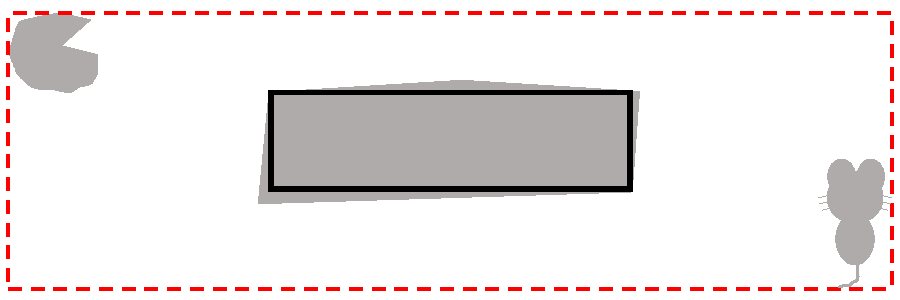
\includegraphics[width=3in]{fig.pdf}
\caption{Example where the underlying distribution $p$ is uniform over the (gray) valid regions. The solid rectangle maximizes our objective since it does not output nonsense (is supported only within the grey matter) and is closest to the $p$ (covers the maximum amount of grey matter). In contrast, the standard maximum likelihood (dashed red) rectangle must fully contain the observed samples, thus generating invalid points most of the time.  }
\end{figure}

Motivated by these observations, we evaluate a generative model $q$ on two axes. First is {\em coverage}, which is related to the probability assigned to future examples drawn from the true distribution $p$. Second is {\em validity}, defined as the probability that random examples generated from $q$ meet some validity requirement. Formally, we measure coverage in terms of a bounded {\em loss}:
$$\Loss(p,q)=\E_{x \sim p}[L(q_x)],$$
where $L:[0,1]\rightarrow [0,M]$ is a bounded decreasing function such as the capped log-loss $L(q_x)=\min(M, \log 1/q_x)$. % or $L(q_x)=\log 1/(q_x+\exp(-M))$. 
A bounded loss has the advantages of being efficiently estimable, and also it enables a model to assign 0 probability to one example (e.g., an outlier or error) if it greatly increases the likelihood of all other data. Validity is defined with respect to a set $V \subseteq X$, and $q(V)$ is the probability that a random example generated from $q$ lies within $V$. 

Clearly, there is a tradeoff between coverage and validity. We first focus on the case of (near) perfect validity. A Valid Generative Modeling (VGM) algorithm if it outputs, for a family of distributions $Q$ over $X$, if it outputs $\hat{q}$ with (nearly) perfect validity and whose loss is nearly as good as the loss of the best valid $q\in Q$. More precisely, $A$ is a VGM learner of $Q$ if for any nonempty valid subset $V \subseteq X$, any probability distribution $p$ over $V$, and any $\eps>0$, $A$ uses $n$ random samples from $p$ and makes $m$ membership oracle calls to $V$ and outputs a distribution $\hat{q}$ such that, $$\Loss(p, \hat{q}) \leq \min_{q \in Q: q(V)=1}\Loss(p,q) + \eps ~\text{ and }~\hat{q}(V)\geq 1-\eps.$$ 
We aim for our learner to be sample and query efficient, requiring that $n$ and $m$ are polynomial in $M, 1/\eps$ and a measure of complexity of our distribution class $Q$.
Furthermore, we would like our algorithms to be computationally efficient, with a runtime polynomial in the size of the data, namely the $n + m$ training examples. 
A more formal description of the problem is available in Section~\ref{sec:problem}.

$A$ is said to be {\em proper} if it always outputs $\hat{q}\in Q$ and {\em improper} otherwise.
In Section~\ref{sec:impossibility}, we first show that efficient proper learning for VGM is impossible. This is an information-theoretic result, meaning that even given infinite runtime and positive samples, one still cannot solve the VGM problem. Interestingly, this is different from binary classification, where it is possible to statistically learn from iid examples without a membership oracle.

Our first main positive result is an efficient (improper) learner for VGM. The algorithm relies on a subroutine that solves the following {\em Generative Modeling with Negatives} (GMN) problem: given sets $X_P, X_N \subset X$ of positive and negative examples, find the probability distribution $q \in Q$ which minimizes $\sum_{x \in X_P} L(q(x))$ subject to the constraint that $q(X_N)=0$. For simplicity, we present our algorithm for the case that the distribution family $Q$ is finite, giving sample and query complexity bounds that are logarithmic in terms of $|Q|$. However, as we show in Section~\ref{sec:infinite-families}, all of our results extend to infinite families $Q$. It follows that if one has a computationally efficient algorithm for the GMN problem for a distribution family $Q$, then our reduction gives a computationally efficient VGM learning algorithm for $Q$.

Our second positive result is an algorithm that minimizes $\Loss(p,q)$ subject to a relaxed validity constraint comparing against the optimal distribution that has validity $q(V)$ at least $1-\alpha$ for some $\alpha>0$. We show in Section~\ref{sec:partial-validity} that even in this more general setting, it is possible to obtain an algorithm that is statistically efficient but may not be computationally efficient. An important open question is whether there exists a computationally efficient algorithm for this problem when given access to an optimization oracle, as was the case for our algorithm for VGM.

\subsection{Related Work}
\cite{KearnsMRRSS94} showed how to learn distributions from positive examples in the realizable setting, i.e., where the true distribution is assumed to belong to the class being learned. In the same sense as their work is similar to PAC learning \citet{Valiant84} of distributions, our work is like agnostic learning \citet{KearnsSS94} in which no assumption on the true distribution is made. 

Generative Adversarial Networks (GANs)~\cite{GoodfellowPMXWOCB14} are an approach for generative modeling from positive examples alone, in which a generative model is trained against a discriminator that aims to distinguish real data from generated data. In some domains, GANs have been shown to outperform other methods at generating realistic-looking examples. Several shortcomings of GANs have been observed \citet{AroraRZ18}, and GANs are still subject to the theoretical limitations we argue are inherent to any model trained without a validity oracle. 

In supervised learning, there is a rich history of learning theory with various types of queries, including membership which are not unlike our (in)validity oracle. Under various assumptions, queries have been shown to facilitate the learning of complex classes such as finite automata \citet{Angluin88} and DNFs \citet{Jackson97}. See the survey of \cite{Angluin92} for further details.  Interestingly, \cite{Feldman09} has shown that for agnostic learning, i.e., without making assumptions on the generating distribution, the addition of membership queries does not enhance what is learnable beyond random examples alone. 
Supervised learning also has a large literature around active learning, showing how the ability to query examples reduces the sample complexity of many algorithms. See the survey of \cite{Hanneke14}. Note that the aim here is typically to save examples and not to expand what is learnable.
 
More sophisticated models, e.g., involving neural networks, can mitigate the invalidity problem as they often generate more realistic natural language and have even been demonstrated to generate \LaTeX{} that nearly compiles \citep{Karpathy15} or nearly valid Wikipedia markdown. However, longer strings generated are unlikely to be valid. For example, \cite{Karpathy15} shows generated markdown which includes:
\begin{quote}
==Access to ''rap===
The current history of the BGA has been [[Vatican Oriolean Diet]], British Armenian, published in 1893.  While actualistic such conditions such as the [[Style Mark Romanians]] are still nearly not the loss.
\end{quote}

Even ignoring the mismatched quotes and equal signs, note that this example has two so-called ``red links'' to two pages that do not exist. Without checking, it was not obvious to us whether or not Wikipedia had pages titled {\em Vatican Oriolean Diet} or {\em Style Mark Romanians}. In some applications, one may or may not want to disallow red links. In the case that they are considered valid, one may seek a full generative model of what might plausibly occur inside of brackets, as the neural network has learned in this case. If they are disallowed, a model might memorize links it has seen but not generate new ones. A validity oracle can help the learner identify what it should avoid generating.

 In practice, \cite{KusnerPH17} discuss how generative models from neural networks (in particular autoencoders) often generate invalid sequences. 
\cite{JanzWPKH18} learn the validity of examples output by a generative model using oracle feedback. 


\section{Property Testing Background and Models}
\label{sec:model}
\subsection{Query Testing (Standard Property Testing)}
Given functions $f$ and $g$ over domain $X$, we define the distance between $f$ and $g$ with respect to distribution $\calD$ over $X$ to be
\begin{equation}
\dist_\calD(f,g)=\Pr_{x\sim\calD}[f(x)\neq g(x)].
\end{equation}
Given a class $\calC$ of functions over domain $X$ and a margin $\epsilon$, a \emph{property tester} distinguishes the case that the input function $f$ is in the class $\calC$ from the case that $f$ is $\epsilon$-far from $\calC$:
\begin{enumerate}
\item if $f\in\calC$, the tester accepts $f$ with probability at least $\frac{2}{3}$;
\item if $\forall g\in\calC,\dist_\calD(f,g)>\epsilon$, the tester rejects $f$ with probability at least $\frac{2}{3}$.
\end{enumerate}
\citet{RS96} first studied the property testing model assuming $X$ is finite and $\calD$ is uniform. We call the testing model of \citet{RS96} as \emph{query testing}, because the tester makes queries to access $f$, i.e., the tester asks for the value of $f(x)$ for some $x\in X$ for each query it makes.

\citet{PRR06} first studied the \emph{tolerant} version of property testing: given an additional parameter, the threshold $\alpha$, to distinguish a function $\alpha$-close to the class from a function $(\alpha+\epsilon)$-far from the class. In other words, 
\begin{enumerate}
\item if $\exists g\in \calC,\dist_\calD(f,g)\leq\alpha$, the tester accepts $f$ with probability at least $\frac{2}{3}$;
\item if $\forall g\in\calC,\dist_\calD(f,g)>\alpha+\epsilon$, the tester rejects $f$ with probability at least $\frac{2}{3}$.
\end{enumerate}
They showed tolerant testers for clustering and for monotonicity in the query testing model. \citet{FF05} showed the existence of classes of binary functions that are efficiently query-testable in the non-tolerant case but are not efficiently query-testable in the tolerant case.

\citet{PRR06} also considered a similar task called distance approximation: estimating the distance from the function to the class so that with probability at least $\frac 23$ the output is within $\pm\epsilon$ to the true distance. Note that distance approximation with additive error $\epsilon$ implies tolerant testing with margin $2\epsilon$ with the same query complexity. Based on this observation, all the tolerant testers we design in this paper actually perform distance approximation (so we don't need the parameter $\alpha$) because distance approximation is a slightly more convenient model for our presentation.
\subsection{Passive Testing (Sample-Based Testing)}
\label{subsec:passive}
\citet{GGR98} first studied testers with the ability to obtain a random sample in addition to making queries so that the tester can potentially work on arbitrary distributions (see Section \ref{subsec:distributionfree} for distribution-free testing), although their algorithmic results remained in the query testing framework over the uniform distribution.
\citet{KR98} developed the first \emph{passive} testers, testers that don't make queries and only rely on the random i.i.d.\ sample to access the input function $f$, for a variety of classes with sub-learning sample complexity. \citet{GR13} advanced the study of passive testers by providing several general positive results as well as by revealing relations with other testing models.

\emph{Proper} learning implies testing, simply by testing using the output hypothesis, but passive testing can be substantially harder than \emph{improper} learning. \citet{GGR98} pointed out that the class of $k$-term-DNF is NP-hard for non-tolerant passive testing while it is efficiently PAC learnable via $k$-CNF \citep{PV88}, if we require testing and learning on an arbitrary distribution.

The general hardness of \emph{tolerant} passive testing based on hardness of improper \emph{agnostic} learning can be implied from the recent work by \citet{KL18}. They considered the task of refutation: for any fixed distribution $\calD$ over domain $X$, given a sample of example-label pairs $\{(x_i,y_i)\}$ and margin $\epsilon>0$, to distinguish the following two cases:
\begin{enumerate}
\item accept when every $(x_i,y_i)$ is i.i.d.\ from some distribution $\calD'$ over $X\times\{0,1\}$ with marginal on $X$ being $\calD$ and $\exists f\in\calC,\Pr_{(x,y)\sim\calD'}[f(x)\neq y]\leq\frac 12-\epsilon$;
\item reject when every $x_i$ is i.i.d.\ from $\calD$ and every $y_i$ is i.i.d.\ from the uniform distribution over $\{0,1\}$.
\end{enumerate}
They showed that a refutation algorithm for distribution $\calD$ with margin $\epsilon$ and sample complexity $s$ implies an improper agnostic learning algorithm for the same distribution with error $3\epsilon$ and sample complexity $O(\frac{s^3}{\epsilon^2})$. We show in Appendix \ref{sec:refutation} that the refutation algorithm can be reduced to a tolerant passive tester for arbitrary unknown distributions with threshold $\alpha=\frac 12-\frac{3\epsilon}4$, margin $\frac{\epsilon}{2}$, and sample complexity $\Omega(s)$, implying that tolerant passive testing for arbitrary unknown distributions can't be substantially more sample-efficient than improper agnostic learning for any distribution $\calD$ (with some reasonable assumptions about the distribution $\calD$). %The reduction also has a uniform-distribution version (Lemma \ref{}), implying the hardness of tolerant passive testing over the uniform distribution.

%\citet{Vad17} showed that if one can perform refutation, i.e., distinguishing a function in the class from a random function, using a sample of size $s$, then one can also do improper PAC learning with sample complexity $O(\poly(s))$.  \citet{KL18} showed similar results for the tolerant (agnostic) case. They used a different definition of refutation: distinguishing a function having distance $\frac 12-\epsilon$ to the class from a random function, and showed that if one can perform refutation using a sample of size $s(\epsilon)$, then one can also do improper agnostic learning with sample complexity $O(\frac{\left(s(\frac\epsilon 2)\right)^3}{\epsilon^2})$.\footnote{One difference between the two results is that \citet{Vad17} assumes that the distribution is arbitrary while the result by \citet{KL18} is distribution-specific. } Note that passive testing implies refutation with the same sample complexity both in the non-tolerant and the tolerant case, assuming the concept class has a finite VC-dimension and the distribution has no massive points so that a random function has distance $\frac 12$ to it with probability 1. Therefore these results imply that passive testing can't be substantially more sample-efficient than improper learning.

\subsection{Active Testing}
Both query testing and passive testing have shortcomings. The assumption of query testing that the tester can make queries to arbitrary points in the domain is usually impractical, while passive testing is too restrictive: for the tolerant case, passive testing can't be substantially more sample-efficient than agnostic learning (recall Section \ref{subsec:passive}).

To avoid both shortcomings, \citet{BBBY12} proposed the active testing model where the tester first receives an unlabeled random i.i.d.\ sample and then makes queries to points in the sample. While the size of the unlabeled sample might be comparable to the labeled sample complexity for learning, the number of queries the tester makes should be substantially smaller.
%large (but is still required to be polynomial in the VC-dimension of the class), the number of queries the tester makes should be substantially smaller than the sample complexity for learning. 
They showed (non-tolerant) active testers for unions of $d$ intervals and for linear separators.
\subsection{Distribution-Free Testing}
\label{subsec:distributionfree}
Distribution-free testing \citep{GGR98} considers testers that work on arbitrary unknown distributions with the ability to obtain random i.i.d.\ sample in addition to making queries. \citet{HK03} designed distribution-free testers for low-degree multivariate polynomials, monotone functions, and several other classes.

The difference between distribution-free testing and passive testing (over arbitrary unknown distributions) is that distribution-free testers have the ability to make queries while passive testers don't. However, the query ability is helpful only when we do \emph{non-tolerant} testing where the tester is only required to accept functions in the class, rather than functions having distance 0 to the class with respect to the unknown distribution. For \emph{tolerantly} testing binary functions, we show that distribution-free testing implies passive testing with the same sample complexity (see Section \ref{sec:relationship} Lemmas \ref{lm:distributionfreenontolerant} and \ref{lm:distributionfreetolerant}) and thus the hardness for tolerant passive testing extends automatically to tolerant distribution-free testing.



%\subsection{Property Testing, Tolerant Testing and Distance Approximation}
%Suppose we have a ground set $X$ and a distribution $\calD$ over $X$. For any two binary functions $f,g\in\{0,1\}^X$, we define their distance to be $\dist_{\calD}(f,g)=\Pr_{x\sim \calD}[f(x)\neq g(x)]$. 

%Suppose we also have a concept class $\calC\subseteq\{0,1\}^X$. Given a function $f\in\{0,1\}^X$ and a margin $\epsilon$ as input, the task of property testing $\pt_{\calD}(f,\epsilon)$ \citep{RS96} is to distinguish the case that $f$ belongs to class $\calC$ from the case that $f$ is $\epsilon$-far from $\calC$. In other words, $\forall f$,
%\begin{enumerate}
%\item if $f\in\calC$, the algorithm outputs ``YES'' with probability at least $\frac{2}{3}$;
%\item if $\forall g\in\calC,\dist_{\calD}(f,g)>\epsilon$, the algorithm outputs ``NO'' with probability at least $\frac{2}{3}$.
%\end{enumerate}
%A property testing algorithm may be randomized, and in this case, the goal is to output the correct answer with probability at least $\frac{2}{3}$. The success probability can be boosted to $1-\delta$ by repeating the algorithm for $O(\log\frac{1}{\delta})$ times and taking the majority.

%The function $f$ can be given to the algorithm in many different ways. In the \emph{query testing} framework \citep{RS96}, the algorithm can query the value of $f(x)$ for any $x\in X$. In this framework, we say the algorithm has \emph{query access} to $f$, or has access to $f\qu$. The query complexity of the algorithm, as a function of $\frac{1}{\epsilon}$, is measured by the maximum number of queries needed by the algorithm.

%\citet{BBBY12} argued that the query testing framework is not realistic for machine learning practice. They proposed the \emph{active testing} framework, in which the algorithm first requests $N$ unlabeled examples $x_1,x_2,\cdots,x_{N}\in X$ sampled independently according to $\calD$ and can only choose to query $f(x_i)$ for $1\leq i\leq N$. In this framework, we say the algorithm has \emph{active access} to $f$, or has access to $f\ac$. The maximum value of $N$, as a function of $\frac{1}{\epsilon}$, is called the \emph{unlabeled sample complexity}. The query complexity is still defined as a function of $\frac{1}{\epsilon}$ measuring the maximum number of queries needed by the algorithm.

%\citet{GGR98} and \citet{KR98} studied an even more strict way of accessing $f$, called \emph{passive access}, in which the algorithm is given the label of an example chosen independently at random from $\calD$ for each query the algorithm makes. 

%Tolerant testing $\tot_{\calD}(f,\alpha,\epsilon)$ \citep{PRR06} is a similar task to property testing. The only difference is that besides the margin $\epsilon$, we are given another parameter $\alpha$ as input, and we are asked to distinguish the case that $f$ is $\alpha$-close to $\calC$ from the case that $f$ is $(\alpha+\epsilon)$-far from $\calC$. %following two cases:
%\begin{enumerate}
%\item $\exists g\in\calC,\dist_{\calD}(f,g)\leq \alpha$;
%\item $\forall g\in\calC,\dist_{\calD}(f,g)>\alpha+\epsilon$.
%\end{enumerate} 
%The query complexity of tolerant testing is still measured as a function of $\frac{1}{\epsilon}$ \citep{PRR06}. 

%A natural generalization of tolerant testing is distance approximation, in which we are only given the function $f$ and the margin $\epsilon$ as input and required to output $\hat\alpha$ as an approximation of the distance from $f$ to $\calC$ up to an additive error $\epsilon$. More specifically, the goal of $\da_{\calD}(f,\epsilon)$ is to output $\hat\alpha$ such that $\forall f$,
%\begin{enumerate}
%\item $\forall \alpha$ such that $\exists g\in\calC,\dist_{\calD}(f,g)\leq \alpha$, it holds with probability at least $\frac{2}{3}$ that $\hat\alpha\leq \alpha+\epsilon$;
%\item $\forall \alpha$ such that $\forall g\in\calC,\dist_{\calD}(f,g)>\alpha$, it holds with probability at least $\frac{2}{3}$ that $\hat\alpha> \alpha-\epsilon$.
%\end{enumerate}

%The success probability of a distance approximation algorithm can be boosted to $1-\delta$ by repeating it $O(\log\frac{1}{\delta})$ times and taking the median. 

%Because for any $\calD$ and $\epsilon$, it's clear that a $\da_{\calD}(f,\frac{\epsilon}{2})$ algorithm implies a $\tot_{\calD}(f,\alpha,\epsilon)$ algorithm with the same query and unlabeled sample complexity \citep{PRR06}, we focus on distance approximation rather than tolerant testing throughout the paper.

%For all of the above examples, the distribution $\calD$ appears in the subscript meaning that the distribution is fixed and known to the algorithm. In this paper, we will consider a more general case, for example $\pt(f\qu,\epsilon,\calD)$, in which the distribution $\calD$ is arbitrarily given to the algorithm as input. When the algorithm has active or passive access to $f$, it's possible to consider an even more general case, for example $\pt(f\ac,\epsilon)$, in which the distribution $\calD$ is unknown to the algorithm (but implicitly given to the algorithm when accessing $f$).




%We use $q^{\text{query}}(\epsilon)$ and $q^{\text{active}}(\epsilon)$ to denote the maximum number of queries needed in the query testing model and the active testing model, respectively. \citet{BBBY12} showed that $q^{\text{query}}(\epsilon)\leq q^{\text{active}}(\epsilon)$ always holds for non-tolerant property testing, which can be easily generalized to tolerant testing and distance approximation. They also showed for non-tolerant property testing that when $\calC$ is the class of dictator functions and $\calD$ is the uniform distribution over $\{0,1\}^p$, there is a testing algorithm in the query testing framework whose query complexity $q^{\text{query}}(p,\epsilon)$ does not grow with respect to $p$, while every testing algorithm in the active testing framework requires $q^{\text{active}}(p,\epsilon)=\Omega(\log p)$ queries for any fixed $0<\epsilon<\frac{1}{2}$.

%In this paper, however, we will show in Theorem \ref{thm:unlabeled} a reversed inequality that $q^{\text{active}}(\epsilon)=O(q^{\text{query}}(\frac{\epsilon}{2}))$ when we are required to do testing on \emph{arbitrary} distribution $\calD$ and the queries are required to lie in the support of $\calD$ (when we have query access)\footnote{We can assume without loss of generality that the queries all lie in the support of $\calD$ when we do tolerant testing and distance approximation, but we cannot assume this for non-tolerant property testing. The reason is that $f\in\calC$ is stronger than $\exists g\in\calC,\dist_{\calD}(f,g)=0$.}, uncovering the relationship between query access and active access.


%Similar to Theorem \ref{thm:unlabeled}, we have the following theorem in tolerant testing. Its proof is a simple modification of the proof to Theorem \ref{thm:unlabeled}.






\documentclass[final,12pt]{colt2018} % Anonymized submission
% \documentclass{colt2017} % Include author names

% The following packages will be automatically loaded:
% amsmath, amssymb, natbib, graphicx, url, algorithm2e

\title[Learning Single-index Models]{Learning Single-Index Models in Gaussian Space}
\usepackage{times}
\usepackage{amsfonts,amssymb,amsmath,graphicx,float,spverbatim,listings,bm,comment,stackrel} % Cannot have "fullpage" package, also not sure if "mathpazo" is okay.
\usepackage{pdflscape,rotating,lscape,wrapfig,color,tcolorbox}
\usepackage{algorithm2e,color}
\usepackage{cleveref}
\lstset{
	basicstyle=\small\ttfamily,
	columns=flexible,
	breaklines=true
}
\DeclareMathOperator{\sech}{sech}
\usepackage{algorithm,algorithmic}
\newcommand{\N}{\mathbb{N}}
\newcommand{\E}{\mathbb{E}}
\newcommand{\Prob}{\mathbb{P}}
\newcommand{\Z}{\mathbb{Z}}
\newcommand{\Q}{\mathbb{Q}}
\newcommand{\R}{\mathbb{R}}
\newcommand{\place}[2]{%
  \overset{\stackrel{#1\\\smile}}{#2}%
}
\newcommand{\sd}[1]{\text{OD}(#1)}
\newcommand{\var}[1]{ \text{Var} \left( #1 \right)}
\newcommand{\unitsphere}[1]{\mathbb{S}^{#1}}
\newcommand{\tv}[2]{\textbf{TV}\left(#1,#2\right)}
\newcommand{\iid}{\stackrel{\text{i.i.d.}}{\sim}}
%\newcommand{\explain}[2]{\overset{\text{\tiny{#1}}}{#2}}
\newcommand{\explain}[2]{\mathrel{\overset{\makebox[0pt]{\mbox{\normalfont\tiny\sffamily #1}}}{#2}}}
\newcommand{\eqdist}{\stackrel{\text{d}}{=}}
\newcommand{\gauss}[2]{\mathcal{N}\left( #1,#2 \right)}
\renewcommand\v[1]{{\ensuremath{\boldsymbol{#1}}}}
\newcommand\ip[1]{\left\langle #1 \right\rangle}
\newcommand \mess[4]{#1_{#2 \rightarrow #3}^{#4}}
\newcommand \norm[1] {{\ensuremath{\|#1\|_2}}}

\newcommand\independent{\protect\mathpalette{\protect\independenT}{\perp}}
\def\independenT#1#2{\mathrel{\rlap{$#1#2$}\mkern2mu{#1#2}}}
\usepackage{dsfont}
\newtheorem{problem}{Problem}
\newtheorem{countereg}{Counter Example}
\newtheorem{gap}{Gap}
\newtheorem{fact}{Fact}
\newtheorem{question}{Question}
\newtheorem{assumption}{Assumption}
\newcommand*\diff{\mathop{}\!\mathrm{d}}
\newcommand{\indicator}[1]{\mathds{1}\{#1\}}
\newcommand{\bigoh}[1]{\mathcal{O}\left( #1 \right)}
\newcommand{\lambdamin}[1]{\lambda_{\text{min}} \left( #1 \right)}
\newcommand{\lambdamax}[1]{\lambda_{\text{max}} \left( #1 \right)}
%for doing case analysis
\newcounter{casenum}
\newenvironment{caseof}{\setcounter{casenum}{1}}{\vskip.5\baselineskip}
\newcommand{\case}[2]{\vskip.5\baselineskip\par\noindent {\bfseries Case \arabic{casenum}:} #1\\#2\addtocounter{casenum}{1}}

%\usepackage[textsize=tiny]{todonotes}
\usepackage[disable]{todonotes}
\newcommand{\todod}[2][]{\todo[color=blue!20!white,#1]{D: #2}}
\newcommand{\todor}[1]{{\color{red} #1}}
\crefname{lemma}{Lemma}{Lemmas}
 % Use \Name{Author Name} to specify the name.
 % If the surname contains spaces, enclose the surname
 % in braces, e.g. \Name{John {Smith Jones}} similarly
 % if the name has a "von" part, e.g \Name{Jane {de Winter}}.
 % If the first letter in the forenames is a diacritic
 % enclose the diacritic in braces, e.g. \Name{{\'E}louise Smith}

 % Two authors with the same address
  % \coltauthor{\Name{Author Name1} \Email{abc@sample.com}\and
  %  \Name{Author Name2} \Email{xyz@sample.com}\\
  %  \addr Address}

 % Three or more authors with the same address:
 % \coltauthor{\Name{Author Name1} \Email{an1@sample.com}\\
 %  \Name{Author Name2} \Email{an2@sample.com}\\
 %  \Name{Author Name3} \Email{an3@sample.com}\\
 %  \addr Address}


 % Authors with different addresses:
 \coltauthor{\Name{Rishabh Dudeja} \Email{rd2714@columbia.edu}\\
 \addr Department of Statistics, Columbia University
 \AND
 \Name{Daniel Hsu} \Email{djhsu@cs.columbia.edu}\\
 \addr Computer Science Department, Columbia University
 }

\begin{document}

\maketitle

\begin{abstract}
We consider regression problems where the response is a smooth but non-linear function of a $k$-dimensional projection of $p$ normally-distributed covariates, contaminated with additive Gaussian noise. The goal is to recover the range of the $k$-dimensional projection, i.e., the index space. This model is called the multi-index model, and the $k=1$ case is called the single-index model. For the single-index model, we characterize the population landscape of a natural semi-parametric maximum likelihood objective in terms of the link function and prove that it has no spurious local minima. We also propose and analyze an efficient iterative procedure that recovers the index space up to error $\epsilon$ using a sample size $\tilde{O}(p^{O(R^2/\mu)} + p/\epsilon^2)$, where $R$ and $\mu$, respectively, parameterize the smoothness of the link function and the signal strength. When a multi-index model is incorrectly specified as a single-index model, we prove that essentially the same procedure, with sample size $\tilde{O}(p^{O(kR^2/\mu)} + p/\epsilon^2)$, returns a vector that is $\epsilon$-close to being completely in the index space.
\end{abstract}

\begin{keywords}
Single-index models, multi-index models, non-convex optimization, semi-parametric models.
\end{keywords}

\section{Introduction}
Suppose we are given $n$ data points $\{(\v x_i, y_i)\}_{i=1}^n$ generated independently from the following regression model:
\begin{align}
    \v x_i \sim \gauss{\v 0}{\v I_p}, \quad \epsilon_i \sim \gauss{0}{\sigma^2}, \quad y_i = f(\v x_i) + \epsilon_i, \quad \epsilon_i \independent \v x_i . \label{model: our_model}
\end{align}
Here, $\v x_i \in \R^p$ are $p$-dimensional covariates or features and $y_i \in \R$ are the response variables. The function $f: \R^p \rightarrow \R$ is assumed to be smooth and unknown. In many applications of practical interest the function $f$ is not an arbitrary $p$-variate function but depends on  an \emph{unknown} $k$ dimensional projection of $\v x$, that is,
\begin{align}
    f(\v x) & = g(\ip{\v u_1^\star, \v x}, \ip{\v u_2^\star, \v x}, \dotsc, \ip{\v u_k^\star, \v x}) , \label{model: multiindex}
\end{align}
where $g: \R^k \rightarrow \R$ and $\v u_1^\star, \v u_2^\star, \dotsc, \v u_k^\star$ are orthonormal vectors in $\R^p$. In the statistics community, this model is called the multi-index model. The special case $k=1$ is called the single-index model; a simple example is the phase retrieval problem for real signals where $g(z) = z^2$.
We note that in the multi-index model, the index vectors are themselves unidentifiable. However one can hope to identify the span of index vectors which we denote as $\mathcal{\v U}^\star\explain{def}{=}\text{Span}(\v u_1^\star, \v u_2^\star, \dotsc, \v u_k^\star)$.

We study the index model from a semiparametric point-of-view: the parameter of interest is the subspace $\mathcal{U}^\star$ and the link function $g$ is treated as an unknown nuisance parameter. The advantages of taking this view are two-fold. First, designing procedures which make weak assumptions on the link function $g$ are robust to misspecification of the link function. Second, this point of view allows us to study the problem of \emph{representation learning} or \emph{feature engineering} in a simple setting. If one is successfully able to estimate the transformation $\v x \mapsto (\ip{\v u_1^\star, \v x}, \dotsc, \ip{\v u_k^\star, \v x})$, there is hope of avoiding the curse of dimensionality in $p$ dimensions and incurring a curse of dimensionality only in $k$ dimensions.

There is a long line of work studying this model in statistics and machine learning. However existing works suffer from one or more of the following drawbacks:
\begin{enumerate}
     \item Some procedures derive estimators that are solutions to highly non-convex optimization problems. It is unclear when these optimization problems are tractable. 
    \item Some existing procedures make \emph{ad-hoc} assumptions on the unknown link function $g$. These assumptions seem to be required for specific procedures to work and don't seem to capture the inherent statistical difficulty of the problem. 
    \item The sample complexity analysis of some procedures suppresses the dependence of the ambient dimension $p$ in the constants, which makes it unclear whether the sample complexity is polynomial or exponential in $p$. 
\end{enumerate}

In this paper we attempt to address some of these shortcomings. Our main contributions are summarized as follows: 

\begin{enumerate}
    \item For the single-index model, $k=1$, we provide an explicit formula for the population loss of a natural semiparametric maximum likelihood estimate (SMLE). We show that the population loss has no spurious minima. However it may have degenerate critical points. \todod{``Moreover, we explicitly characterize the saddle points [\ldots], which we exploit in the design of a new procedure, discussed below.''} In Theorem~\ref{theorem: landscape_population_loss}, we explicitly characterize the degeneracy of these critical points in terms of a single parameter corresponding to the unknown link function called the Order of Degeneracy of $g$. 
    \item Motivated by our analysis of population loss of the SMLE, we design an easy-to-analyze procedure to recover the index vector for the single-index model. In Theorem \ref{theorem: learn_sim_algo}, we analyze the sample complexity of our procedure in terms of statistically motivated parameters $R^2$ and $\mu$ which quantify the smoothness and signal strength of the link function $g$; see Assumptions~\ref{assumption: smoothness} and~\ref{assumption: min_sig_strength} for their definitions. Our procedure (\Cref{algorithm: learn_sims}) requires $\tilde{\mathcal{O}}(p^{\mathcal{O}(R^2/\mu)} +~ p/\epsilon^2)$ samples where the $\tilde{\mathcal{O}}$ notation suppresses factors polynomial in $1/\delta,\ln(1/\epsilon)$ and  $(R^2/\mu)^{R^2/\mu}$ to return an estimate $\hat{\v u}$ that satisfies $\min(\| \hat{\v u} - \v u^\star \|_2,\| \hat{\v u} + \v u^\star \|_2) \leq \epsilon$ with probability $1-O(\delta) - o_n(1) - o_p(1)$. Furthermore, our procedure runs in time $\bigoh{np}$. Our procedure is a natural higher order generalization of ADE \citep{brillinger2012generalized} and PHD \citep{li1992principal} estimators.
    %\todor{Discuss comment here}
    
    \item For the multi-index case, in Theorem \ref{theorem: multiindex_landscape}, we show that the same procedure can be seen as optimizing an objective which has the desirable property that (nearly) every local extrema in the population objective is an element of the $\mathcal{\v U}^\star$. Finally, in Theorem \ref{theorem: multi_index_algo_analysis}, we show that with $\tilde{\mathcal{O}}(p^{\mathcal{O}(kR^2/\mu)}/\epsilon^2)$ samples, the procedure returns an estimate $\hat{\v u}$ such that $\|\mathcal{P}_{\mathcal{\v U}^\star}( \hat{\v u})\|_2 \geq 1 - \epsilon$. This means that our procedure for learning single-index model is robust even when a multi-index model is misspecified as a single-index model.
\end{enumerate}

\subsection{Related Work}

There is a large literature dealing with estimation of index models. We briefly review the different approaches mentioning some representative papers for each approach. 
\paragraph{Semiparametric Maximum Likelihood Estimators:}
A well known estimator for the index vector is the semiparemetric maximum likelihood estimator (SMLE). The basic idea behind SMLE is as follows: Suppose our best guess for the index vectors was $\v u_1, \v u_2, \dotsc, \v u_k$. Given this guess, one could estimate the link function $g$ using a non-parametric estimator such as a kernel smoothing estimator with bandwidth $h: \hat{g}_{h}(\ip{\v u_1,\v x}, \dotsc, \ip{\v u_k,\v x})$. One could also evaluate how good our guess for the index vectors was using a suitable goodness-of-fit statistic such as the Sum-of-Squared Errors %(SSE):
%\begin{align*}
%    \text{SSE}(\v u_1 , \dots \v u_k) & = \frac{1}{n} \sum_{i=1}^n (\hat{g}_{h}(\ip{\v u_1,x_i} \dots \ip{\v u_k,x_i}) - y_i)^2.
%\end{align*}
    $\text{SSE}(\v u_1 , \dotsc, \v u_k) = \sum_{i=1}^n (\hat{g}_{h}(\ip{\v u_1,\v x_i}, \dotsc, \ip{\v u_k,\v x_i}) - y_i)^2$.
One can then estimate the index vectors by minimizing the goodness of fit statistic. %:
%\begin{align*}
%    (\hat{\v u}_1^{\text{SMLE}}, \dots, \hat{\v u}_k^{\text{SMLE}}) &= \arg\max_{\v u_1, \dots \v u_k} \frac{1}{n} \sum_{i=1}^n (\hat{g}_{h}(\ip{\v u_1,x_i} \dots \ip{\v u_k,x_i}) - y_i)^2.
%\end{align*}
The SMLE is known to have excellent statistical properties in the asymptotic regime where the ambient dimension $p$ is fixed and the number of samples $n \rightarrow \infty$ such as $\sqrt{n}$-consistency and asymptotic efficiency under \emph{very weak} assumptions on the distribution of covariates. However, it is not clear whether the optimizing the SSE is tractable.  Furthermore, the classical asymptotic analysis does not capture terms in the Mean Squared Error which might be more important in modern day scenarios, where $p$ is often large and comparable to $n$. See the book by \citet{horowitz2009semiparametric} for a nice review on results about the SMLE. 
\paragraph{Gradient-Based Estimators:}
A second approach developed in a series of papers by \citet{hristache2001direct,hristache2001structure,dalalyan2008new} leverages the observation that the gradients $\nabla f(\v x)$ lies in the span of the index vectors and hence $\mathcal{\v U^\star}$ can be estimated by running PCA on non-parametric estimators of the gradients, for example the slope of a local-linear regression estimate:
\begin{align*}
    (\hat f(\v x), \widehat{\nabla f}(\v x))
& = \arg \min_{c \in \R, \beta \in \R^p} \sum_{i=1}^n \left( y_i - c - \ip{ \v \beta, \v x_i - \v x} \right)^2 K_h \left( \| \v x - \v x_i \| \right)
\end{align*}
for some kernel smoothing function $K_h$. The problem with this estimate is that it isn't clear if the estimate of the index vectors derived from this non-parametric gradient estimate would even be $\sqrt{n}$-consistent since the gradients are estimated at a slow rate. However \citet{hristache2001direct,hristache2001structure,dalalyan2008new} show that it is possible to iteratively improve this estimator to get a $\sqrt{n}$-consistent estimator of the span of the index vectors when $k<4$ under very weak assumptions on the distribution of covariates. Furthermore, their procedure is also computationally tractable. However, their analysis suppresses the dependence of $p$ in constant terms. More precisely, they show that estimating the span of the index vectors up to a tolerance $\epsilon$ requires $\bigoh{1/\epsilon^2}$ samples (which is much better than $\bigoh{1/\epsilon^p}$), but this $\bigoh{\cdot}$ suppresses a $2^p$ factor in the sample size.
\paragraph{Moment-Based Estimators:} 
Another line of work makes assumptions on the covariate distribution (e.g., Gaussian or elliptical). Such assumptions permit one to take advantage of Stein's Lemma and its generalizations to derive moment-based estimators for the index vectors. Specifically if $\v x_i \sim \gauss{0}{\v I_p}$, then,
\begin{align*}
    \E[ y \v x] = \E[\nabla f(\v x)], \quad \E[y \v x \v x^T ]  - \E[f(\v x)] \v I_p = \E[\nabla^2 f(\v x)].
\end{align*}
Since for multi-index models, $\E[\nabla f(\v x) ] \in \mathcal{\v U^\star}$ and $\text{Range}(\E[\nabla^2 f(\v x)]) \subset \mathcal{\v U}^\star$, estimates of these moments derived from empirical averages can be used to estimate subspaces of the span of the index vectors. The estimator based on the first moment is called Average Derivative Estimator (ADE) and was proposed by \citet{brillinger2012generalized}. The estimator based on the second moment is called Principal Hessian Directions (PHD) and was proposed by \citet{li1992principal}. More recently, these estimators were revisited by \citet{plan2017high} and \citet{neykov2016agnostic} in the context of single-index models. They analyze these estimators providing non-asymptotic bounds with explicit dependence on $p$. They also extend these estimators to the situation where the index vector has additional structure like sparsity. However, the key drawback of these estimators is that they are not guaranteed to estimate the entire span of the index vectors. For example consider the situation when $k=1$ and $g(z) = H_3(z)$. Here $H_3$ denotes the Hermite Polynomial of degree 3. One can check for this example, $\E[\nabla f(\v x)] = \v 0$ and $\E[\nabla^2 f(\v x)] = \v 0$. Hence both ADE and PHD fail to recover the index vector. The underlying cause for this failure mode is that both ADE and PHD extract index vectors participating in the first two harmonics of the link function $g$ and can miss out on index vectors involved in higher order harmonics of the link function $g$. 
\paragraph{Slicing:}
A partial solution to the failure of moment-based estimators to the entire subspace $ \mathcal{\v U}^\star$ is a technique called Slicing. This technique was introduced in \cite{li1991sliced} and is based on the observation that almost surely with respect to $y$,
\begin{align*}
    \E[\v x | y] \in \mathcal{U}^\star , \quad
    \text{Range}(\E[\v x \v x^T | y]-I) \subset \mathcal{U}^\star  .
\end{align*}
The advantage of slicing is that one can now estimate the sliced moments $\E[\v x |y]$ and $\E[\v x \v x^T | y]$ for a number of different values of $y$ and this hopefully reduces the chance of missing certain relevant directions. However, even Sliced Inverse Regression is guaranteed to consistently capture all the relevant directions under ad-hoc assumptions like:
\begin{align}
    \text{Rank} \left( \E_y \left[ \E\left[\v x | y\right] \E\left[ \v x | y\right] ^T \right]\right) & = k , \label{slicing_assumption_1} \\
    \text{Rank} \left( \E_y \left[ \left(\E\left[\v x \v x^T | y\right]-I\right)^2 \right] \right) & = k . \label{slicing_assumption_2}
\end{align}
For \Cref{slicing_assumption_1}, it is easy to see that the phase retrieval problem violates this assumption since the link function $g(z) = z^2$ is even and hence $\E[\v x|y] = 0$. We are not aware of any counterexamples to  \Cref{slicing_assumption_2} nor a proof that this assumption holds for an arbitrary link function. Due to assumptions like these, the analysis of slicing depends on parameters like the $\lambda_{\text{min}} \left( \E_y \left[ \E\left[\v x | y\right] \E\left[ \v x | y\right] ^T \right] \right)$ and the smoothness of the function $s(y)\explain{def}{=}\E[\v x|y]$. It is not clear how these parameters relate to more natural notions of signal strength for this problem or to the smoothness of the underlying link function. We refer the reader to \cite{babichev2016slice} for a non-asymptotic analysis of Sliced Inverse Regression and a discussion of the failure modes of various slicing strategies.

\paragraph{Other related work:}
Recent concurrent work of \citet{ge2017learning} uses techniques based on Hermite polynomials similar to ours to learn neural networks of the form $\sum_{i=1}^m a_i^\star \sigma(\ip{\v b_i^\star,\v x})$ where $a_i^\star \geq 0$ and $\v b_i$ are linearly independent. They assume that the link function $\sigma$ is known (e.g., ReLU or $\tanh$ activation), and leverage this knowledge to design an objective depending on $\sigma$ that has benign structure (e.g., no spurious local minima or degenerate critical points). Since we take a semi-parametric point-of-view, we are unable to do this. In particular we need to handle objectives with degenerate critical points.

\subsection{Assumptions}
We assume that we have $n$ data points generated the regression model defined in Equation~\eqref{model: our_model} with a multi-index regression function of order $k$ (defined in Equation~\eqref{model: multiindex}). 
We make the following assumptions on the unknown link function (with $\v z \sim \gauss{\v 0}{\v I_k}$):
\begin{assumption}[Normalization] $\E[g^2(\v z)] = 1$.
\label{assumption: normalization}
\end{assumption}

\begin{assumption}[Bounded Link Function]
    $\| g\|_\infty < \infty$.
\label{assumption: bounded_link}
\end{assumption}

\begin{remark} \Cref{assumption: bounded_link} is not strictly required for our analysis. It can be relaxed to allow for link functions such as $g(z) = z^2$ in the case of phase retrieval. This is done in Appendix \ref{relax_boundedness}.
\end{remark}
\begin{assumption}[Smoothness] $g$ is twice differentiable, and $\E [ (\frac{\partial^2 g(\v z)}{\partial z_i \partial z_j})^2 ] \leq R^2$ for all $i,j \in [k]$.
\label{assumption: smoothness}
\end{assumption}

\begin{assumption}[Minimum Signal Strength] 
$\E[( \frac{\partial g(\v z)}{\partial z_i})^2] \geq \mu$ for all $i \in [k]$.
\label{assumption: min_sig_strength}
\end{assumption}

\begin{remark}We note that $\mu$ is a very natural notion of signal strength in this problem. If \Cref{assumption: min_sig_strength} is violated for some coordinate $i \in [k]$, we have
\begin{align*}
    \E \left[ \left( \frac{\partial g(\v z)}{\partial z_i} \right)^2 \right] = 0 \implies \frac{\partial g(\v z)}{\partial z_i} \explain{a.s.}{=} 0 \implies g(z_1, z_2, \dotsc, z_k) = g^\prime(z_1, \dotsc, z_{i-1}, z_{i+1}, \dotsc, z_k).
\end{align*}
This means that the value of the response $y$ is independent of the projection of the covariate along the direction $\v u_i^\star$ and hence, we cannot possibly hope to recover it. 
\end{remark}
% DJH: this is great!


\subsection{Notation}
\paragraph{Notation for Hermite Polynomials:} We will represent the unknown link function using orthogonal polynomials for the Gaussian measure called {\em Hermite polynomials}. Let $H_i(z)$ denote the (normalized) Hermite polynomial of degree $i$. These polynomials form an orthonormal basis for square-integrable univariate functions under the Gaussian measure. Hence, in the case of the single-index model ($k=1$), the unknown link function $g$ admits an expansion in the Hermite polynomial basis of the form: 
\begin{align*}
    g(z) & = \sum_{l=0}^ \infty a_l^\star H_l(z).
\end{align*}
We define the following index sets: $\mathcal{I}_t \explain{def}{=} \{\v S \in (\N \cup \{0\})^k: \sum_{i=1}^k S_i \leq t \}$ and $\mathcal{I}_\infty \explain{def}{=} \bigcup_{t=0}^\infty \mathcal{I}_t$;
and we use the notation $H_{\v S}(\v z)$ for $\v S \in \mathcal{I}_\infty$ to denote the tensor-product Hermite polynomial basis: $H_{\v S}(\v z) \explain{def}{=} \prod_{i=1}^k H_{S_i}(z_i)$.
Analogously, we use the notation $\v z^{\v S}$ for ${\v S} \in \mathcal{I}_\infty$ to denote the monomial: $\v z^{\v S} \explain{def}{=} \prod_{i=1}^k z_i^{S_i}$.
The tensor-product Hermite polynomials form an orthonormal basis for square integrable $k$-variate functions under the product Gaussian measure. Hence for the multi-index model, the unknown link function $g$ admits an expansion of the form: 
\begin{align*}
    g(\v z) & = \sum_{{\v S} \in \mathcal{I}_\infty} a_{\v S}^\star H_{\v S}(\v z).
\end{align*}
\paragraph{Notation for Linear Algebraic Aspects:} For a vector $\v v \in \R^p$, we use $\| \v v \|_1$ to denote the L1 norm and $\| \v v \|_2$ to denote the L2 norm. If the subscript is omitted, $\| \v v \|$ refers to the L2 norm. For matrices, $\| \v A \|$ represents the operator norm. %For vectors $\v u, \v v \in \R^p$, the shorthand $\v v \perp \v u $ means $\ip{\v v , \v u} = 0$.
The notation $\mathcal{P}_{\mathcal{\v U}^\star}$ and $\mathcal{P}^\perp_{\mathcal{\v U}^\star}$ refers to projection operators onto $\mathcal{\v U}^\star$ and the orthogonal complement ${\mathcal{\v U}^\star}^\perp$, respectively. The unit sphere in $\R^p$ is denoted by $\unitsphere{p-1}$. Finally, we define the matrix of orthonormal index vectors $\v U^\star = [\v u_1^\star, \v u_2^\star, \dotsc, \v u_k^\star]  \in \R^{p \times k}$.

\paragraph{Notation for Probabilistic Aspects:} We use the notation $\gauss{\v 0}{\v I_p}$ to represent the standard Gaussian distribution in $p$ dimensions. In particular the statement $\v X \sim \gauss{\v 0}{\v I_p}$ means the random variable $\v X$ is drawn from a $p$-variate standard Gaussian distribution. Analogously $\v u_0 \sim \text{Uniform}(\unitsphere{p-1})$ means that $\v u_0$ is a uniformly random unit vector. 

\paragraph{Outline:} The remaining paper is organized as follows. In Section~\ref{section: landscape analysis} we analyze the landscape of the semi-parametric MLE. We propose a simple objective for the estimating single-index models and analyze its landscape when a multi-index model is misspecified as a single-index one. In Section~\ref{section: single_index} we construct and analyze a procedure to estimate single-index models from finite samples. In Section~\ref{section: multi_index} we analyze the behaviour of this procedure under a multi-index misspecification. We conclude with Section~\ref{section: conclusion} and discuss some open problems. All omitted proofs are in the Appendix. 

\section{Landscape of Some Population Objectives}
\label{section: landscape analysis}
A commonly used estimator for single-index models is the semiparametric MLE which is defined as follows:
\begin{align}
         \hat{\v u} &= \arg\min_{u \in \unitsphere{p-1}} \min_{h \in \mathcal{F}_L} \frac{1}{n} \sum_{i=1}^n(y_i - h(\ip{\v u, \v x_i}))^2. \nonumber
\end{align}
In the above display $\mathcal{F}_L$ is a suitable class of functions from $\R$ to $\R$. The parameter $L$ controls the complexity of the function class and is tuned to achieve an optimal tradeoff between the bias and the variance of the resulting estimator. For example a simple choice for $\mathcal{F}_L$ would be the set of all degree $L$ polynomials: $\mathcal{F}_L = \{g: \R \rightarrow \R, g(z) = \sum_{i=0}^L a_i H_i(z) \}$.
For this function class, the SMLE becomes:
\begin{align}
         \hat{\v u} &= \arg\min_{u \in \unitsphere{p-1}} \min_{\v a \in \R^{L+1}} \frac{1}{n} \sum_{i=1}^n\left(y_i - \sum_{l=0}^L a_l H_l(\ip{\v u, \v x_i})\right)^2 \tag{OPT 1} \label{opt_problem: O1}
\end{align}
It is not clear if Optimization Problem~\ref{opt_problem: O1} is tractable. The first step in understanding its complexity is to understand the landscape of the associated population loss:
\begin{align*}
    R_L(\v u) : = \min_{\v a \in \R^{L+1}} \E \left[ \left(y - \sum_{l=0}^L a_l H_l(\ip{\v u, \v x}) \right)^2 \right].
\end{align*}
It turns out that it is possible to give an explicit expression of the population loss due to a surprising algebraic property of Hermite Polynomials stated below. 
\begin{lemma}[\citealp{o2014analysis}] Let $\v u, \v v$ be unit vectors in $\R^p$. For $\v x \sim \gauss{\v 0}{\v I_p}$, 
\[ \E[H_l(\ip{\v u, \v x}) H_m(\ip{\v v, \v x})] =  \left\{
\begin{array}{ll}
      0 & l\neq m , \\
      \ip{\v u, \v v}^l & l=m .
\end{array} 
\right. \]
\label{lemma: univariate_hermite_key_property}
\end{lemma}

Our first result (Theorem~\ref{theorem: landscape_population_loss}) is that the objective $R_L(\v u)$ has precisely two local minima at $\v u = \pm \v u^\star$. However it may have degenerate critical points. The degeneracy of the critical points of $R_L(\v u)$ is determined by the degree of the smallest non-zero harmonic in the link function $f$. More precisely we define the following notion of the order of degeneracy of $f$:
\begin{definition}[Order of Degenerarcy of $f$] The order of degeneracy of $f$, denoted by $\sd{f}$, is defined as:
$$\sd{f}: = \min \left\{l \in [L]: \E_{x\sim \gauss{0}{\v I_p}}\left[f(\v x) H_l(\ip{\v x, \v u^\star})\right] \neq 0\right\}.$$
\label{definition: saddle_degree}
\end{definition}

\begin{theorem}
\label{theorem: landscape_population_loss} The population loss admits the explicit form: 
$$R_L(\v u)  = \sigma^2 + \sum_{l=1}^L {a_l^\star}^2 (1-\ip{\v u, \v u^\star}^{2l}). $$
The critical points of $ R_L(\v u)$ are given by:
\begin{enumerate}
    \item $\v u = \pm \v u^\star$, which are global minima.
    \item $\v u \in \{ \v a \in \unitsphere{p-1}: \ip{\v a, \v u^\star} = 0\}$. All points in this subspace are global maxima. Furthermore, when $\sd{f}>1$, these local maxima are degenerate, that is, $\nabla^2 R_L(\v u) = \v 0$.
\end{enumerate}
\end{theorem}
%All omitted proofs are given in the appendices.
%\begin{proof}
%This result is restated and proved as Theorem \ref{theorem: landscape_population_loss} in Appendix \ref{section: proofs for landscape analysis}. 
%\end{proof} 



While the objective $R_L(\v u)$ has no spurious local minima, there are a few issues with it:
\begin{enumerate}
    \item Since the objective squares the residuals, it increases the effective order of degeneracy of the function by a factor of two. This increases the number of samples required to guarantee that the landscape of the objective is well-behaved. 
    \item The coefficient vector $\v a$ that minimizes the  objective is dependent on the data. This dependence makes the analysis more complicated. 
\end{enumerate}

To avoid these difficulties, we instead optimize the following objective for some value of $l$ and get an estimate $\hat{\v u}_l$:
\begin{align*}
    \hat{F}_{l}(\v u) &= \frac{1}{n} \sum_{i=1}^n y_i H_l(\ip{\v x_i, \v u}) , \quad
    \hat{\v u}_l = \arg \max_{\v u \in \unitsphere{p-1}} \hat{F}_l(\v u).
\end{align*}
To understand why this objective is reasonable, we consider the population version of the objective: 
\begin{align*}
    F_l(\v u)  %& \quad = \quad  \E \left[ y H_l(\ip{\v x, \v u} \right] \\
      &\quad = \quad  \E \left[f(\v x) H_l(\ip{\v x, \v u}) \right] \\
      & \quad \explain{Lemma~\ref{lemma: univariate_hermite_key_property}}{=} \quad   a_l^\star \ip{\v u, \v u^\star}^l.
\end{align*}
Hence, $F_l(\v u)$ is extremized at $\hat{\v u} = \pm \v u^\star$ provided $a_l^\star \neq 0$. Intuitively, given a harmonic $l$, the objective $F_l(\v u)$ tries to orient the vector $\v u$ in such a way that the energy in this harmonic is maximized. 

\begin{remark}[Degenerate Critical Points] When $l>2$, $F_l(\v u)$ has a degenerate critical points at all $\v u^\perp$ that satisfy $\ip{\v u^\star, \v u^\perp}=0$. In particular, this means that for $l>2$, our objective does not satisfy the strict-saddle \citep{ge2015escaping} or the ridable saddle properties \citep{sun2015nonconvex}. Hence, it is not immediately clear if these generic analysis methods can be applied here. 
\end{remark}

\begin{comment}
\begin{remark}[Connection with Tensor PCA] The empirical version of the objective $\hat{F}_l(\v u)$ will have $\mathcal{O}(1/\sqrt{n})$ fluctuations around the population version. This structure of a degenerate critical point superimposed with $\mathcal{O}(1/\sqrt{n})$ fluctuations is reminiscent of the recent work on Tensor PCA \citep{arous2017landscape} where these fluctuations are known to create exponentially many spurious minima in the empirical objective. Furthermore, for Tensor PCA interesting computational-statistical gaps are well known. Indeed as we shall see in Section~\ref{section: single_index}, estimators based on $F_l(\v u)$ require $\tilde{\mathcal{O}}(p^{\mathcal{O}(R^2/\mu)})$ samples which is likely suboptimal. While this connection is intriguing, it is difficult to established a formal connection between the two problems since the fluctuations from the population objective in our case are not Gaussian as in the Tensor PCA problem. 
\end{remark}
\end{comment}

Let us now consider the situation where a multi-index model of order $k$ was misspecified as a single-index model. One might still hope that optimizing $F_l(\v u)$ does something reasonable. It turns out that the objective $F_l(\v u)$ indeed has this desirable property. One can write an explicit form for  $F_l(\v u)$ when the data is generated by a multi-index model of order $k$. The key tool that allows us to do this is a multivariate analogue of Lemma~\ref{lemma: univariate_hermite_key_property} which is stated below.  
\begin{lemma}
\label{lemma: multivariate_hermite_lemma}
 Let $\v U : = [\v u_1, \v u_2 \dotsc, \v u_k]$ be a matrix in $\R^{p \times k}$ with orthonormal columns. Let $\v v$ be a arbitrary unit vector. Then, 
 \begin{align*}
     1) \quad \E \left[H_{\v S}(\v U x) H_l(\ip{\v v, \v x}) \right] &= 0 &\text{if $l \neq |\v S|$}, \\
     2) \quad \E \left[H_{\v S}(\v U x) H_l(\ip{\v v, \v x}) \right] &= \sqrt{\frac{l!}{S_1 ! S_2 ! \dotsb S_k !}} \prod_{i=1}^k \ip{\v u_i, \v v}^{S_i} &\text{if $l = |\v S|$}.
\end{align*}
\end{lemma}
%\begin{proof}This result is restated and proved as Lemma \ref{lemma: multivariate_hermite_lemma_restated} in Appendix \ref{section: proofs for landscape analysis}. 
%\end{proof}
Our next result (Theorem~\ref{theorem: multiindex_landscape}) characterizes the landscape of the objective $F_l(\v u)$ under a multi-index model and shows that it has no spurious local extrema. 

\begin{theorem} Under the order $k$ multi-index model, the population objective $F_l(\v u)$ has the following properties: 
\begin{enumerate}
    \item The population objective has the following explicit form:
    $$F_l(\v u) = \sum_{{\v S}: \|{\v S}\|_1 = l} a_{\v S}^\star \sqrt{\binom{l}{S_1, S_2, \dotsc, S_k}} \prod_{i=1}^k \ip{ \v u^\star_i, \v u}^{S_i}.$$
    \item Any local maximizer with $F_l(\v u) > 0$ is contained in the subspace $\mathcal{\v U}^\star$. 
    \item Any local minimizer with $F_l(\v u) < 0$ is contained in the subspace $\mathcal{\v U}^\star$.
\end{enumerate}
\label{theorem: multiindex_landscape}
\end{theorem}
%\begin{proof}
%This result is restated and proved as Theorem \ref{theorem: multiindex_landscape_restate} in Appendix \ref{section: proofs for landscape analysis}. 
%\end{proof}
\begin{remark} We note that Theorem~\ref{theorem: multiindex_landscape} falls short of showing that $F_l(\v u)$ has no spurious local minima or maxima. In particular existence of local maxima (or minima) not in $\mathcal{\v U}^\star$ such that $F_l(\v u) = 0$ is not ruled out. However such local maxima are unlikely to be a cause of problems for procedures like gradient ascent (or descent). To see this consider the following procedure: Choose a random initialization point. With probability 1, we will have $F_l(\v u_0) \neq 0$. If the objective is positive, run gradient ascent otherwise run gradient descent. Since gradient ascent with small enough step size is guaranteed to increase the objective, we will never get stuck in a local maxima with $F_l(\v u) = 0$.   
\end{remark}

\section{Learning Single-index Models from Finite Samples}
\label{section: single_index}

In Section~\ref{section: landscape analysis} we showed that the population version of the objective $\hat{F}_l(\v v)$ is extremized at the true index vector $\v u^\star$ provided that the energy of the link function in the harmonic $l$ is not zero ($a_l^\star \neq 0$). In this section, we first design a procedure (Algorithm~\ref{algorithm: fixed_harmonic}) that extracts an estimate of $\v u^\star$ from harmonic $l$ under the promise that $a_l^\star \neq 0$. 

Algorithm~\ref{algorithm: fixed_harmonic} exhibits extremely fast convergence. In particular, it requires only two update steps to return an estimate. The underlying reason behind fast convergence for this algorithm is that the gradient of the population objective is \emph{perfectly} aligned with the index vector $\v u^\star$. The analysis of this procedure is presented in Theorem~\ref{theorem: algo_1_analysis}. At a high level, the analysis of this procedure involved the following steps: 
\begin{enumerate}
    \item Analysis of Random Initialization: We expect a uniformly random unit vector to have a projection of size $\Omega( 1/\sqrt{p})$ on $\v u^\star$. This means that the initialization is very close to a degenerate critical point and hence we see \emph{very small gradients} of size $\bigoh{1/p^l}$
    \item Analysis of the stochastic fluctuations of the gradient: Because our gradients are heavy tailed, this is done via a standard truncation argument. We show that $\| \nabla F_l(\v u) - \nabla \hat{F}_l(\v u)\|_2 \leq \tilde{\mathcal{O}}( \sqrt{p/n} )$. Hence when $n \geq \mathcal{O}({p^l})$, the stochastic fluctuations don't kill off the small gradients we observe at the initialization. This initial sample size requirement of $\bigoh{p^l}$ can be seen as the price to pay to escape the degenerate local critical points. 
    \item Analysis of Iterates: We show that because the gradient of the objective is perfectly aligned with the index vector, $\| \hat{\v u}_l - \v u^\star \|_2 \leq 1$ at the end of the first iteration and $\| \hat{\v u}_l - \v u^\star \|_2 \leq \tilde{\mathcal{O}}( \sqrt{p/n})$ at the end of the second iteration. 
\end{enumerate}

\begin{algorithm}[t]
  \renewcommand\algorithmicrequire{\textbf{input}}
  \renewcommand\algorithmicensure{\textbf{output}}
  \caption{\textsf{Estimate-Index-Vector-from-Harmonic$(S,l)$}}
    \label{algorithm: fixed_harmonic}
  \begin{algorithmic}[1]
    \REQUIRE
    Data $S=\{\v x_i, y_i\}_{i=1}^n \subset \R^p \times \R$;
    Degree of Harmonic $l \in \N$

    \renewcommand\algorithmicrequire{\textbf{assume}}
    
    \ENSURE
    Index Estimate $\hat{\v u}_l \in \R^p$.

    \STATE Split $S$ into two equal parts: \newline
    $S_1: = \{(\v x_i, y_i), i=1,2,\dotsc, \frac{n}{2}\}, S_2: = \{(\v x_i, y_i): i=\frac{n}{2} + 1 , \dotsc, n\}$ \STATE Define
    $\hat{F}_l(\v u; S_1) : = \frac{2}{n} \sum_{i=1}^{\frac{n}{2}} y_i H_l(\ip{\v x_i, \v u})$ and %\newline
    $\hat{F}_l(\v u; S_2) : = \frac{2}{n} \sum_{i=\frac{n}{2}+1}^{n} y_i H_l(\ip{\v x_i, \v u})$ 
    \STATE Random Initialization: 
    $\v u_0 \sim \text{Uniform}(\unitsphere{p-1})$ 
    \STATE Compute two steps of iterative process:
    $\v u_1 = \frac{\nabla \hat{F}_l(\v u_0; S_1)}{\| \nabla \hat{F}_l(\v u_0; S_1)\|_2}$, and then $\v u_2 =\frac{\nabla \hat{F}_l(\v u_1; S_2)}{\| \nabla \hat{F}_l(\v u_1; S_2)\|_2}$.  
\RETURN  $\hat{\v u}_l := \v u_2$
  \end{algorithmic}
\end{algorithm}

\begin{theorem} Given any $\epsilon,\delta \in (0,1)$; with probability $1 - 2\exp(-p/32)-5\delta - \frac{8}{n}$, the output $ \hat{\v u}_l$ of Algorithm 1 satisfies
\begin{align*}
    |\ip{\hat{\v u}_l, \v u^\star}| \geq 1 - \frac{100 (\|f\|_\infty + 4\sigma) \cdot 2^{2l+1}}{l|a_l^\star|} \sqrt{\frac{2\max(p,\ln(1/\delta))\ln^l(n)}{n}},
\end{align*}
provided $n$ is large enough so that the following holds:
\begin{align*}
    \frac{n}{\ln^l(n)} \geq \frac{32\cdot 10^4 (\|f\|_\infty + 4\sigma)^2}{{l^2 a_l^\star}^2} \frac{2^{2l}}{\delta^{2l-2}}\max(p,\ln(1/\delta)) p^{l-1}.
\end{align*}
\label{theorem: algo_1_analysis}
\end{theorem}
%\begin{proof}
%This result is restated and proved as Theorem \ref{theorem: algo_1_analysis_restated} in Appendix \ref{section: single_index_proofs}. 
%\end{proof}
\begin{remark}[Connections to 1-bit Compressed Sensing] Consider the 1-bit compressed sensing problem where $g(z) = \text{sign}(z)$. One can check that for this link function, $a_1^\star = \sqrt{2/\pi}>0$. Hence, when specialized to this case, Theorem \ref{theorem: algo_1_analysis} gives a sample complexity of $O(p\ln(p))$ which is optimal for unstructured signals up to log-factors.
\end{remark}
\begin{remark}[Connections to Phase Retrieval] Consider the phase retrieval problem where $g(z) = z^2 = \sqrt{2}H_2(z) + 1$. A common approach to get an estimate of $\v u^\star$ is by computing the leading eigenvector of the matrix $\widehat{\v M} = \sum_{i=1} y_i \v x_i \v x_i^T$.
Using the variational characterization of the leading eigenvector, one can see that this is exactly the same as optimizing the objective  $\hat{F}_2$. When specialized to this case, Theorem~\ref{theorem: algo_1_analysis} gives a suboptimal sample complexity of $\mathcal{O}(p^2)$, but more specialized analyses of the same estimator using matrix perturbation tools do give the optimal sample complexity of $\mathcal{O}(p)$ \citep[see, e.g.,][]{candes2015phase}.
\end{remark}

We emphasize that Algorithm~\ref{algorithm: fixed_harmonic} succeeds only if we know a harmonic $l$ such that $a^\star_l$ is not too small. In order to design an algorithm that learns single-index models with arbitrary link functions satisfying our assumptions we show that for any such link function, there exists a bounded $l_\sharp \in \N$ such that $a_{l_\sharp}^\star$ is not too small. 

\begin{lemma}[Existence of a good $l_\sharp$] For a link function $g$ that satisfies Assumptions 1, 3 and 4, there exists a $l_\sharp \leq \frac{2R^2}{\mu}$ such that, $l_\sharp |a_{l_\sharp}^\star|^2 \geq \frac{\mu^2}{4R^2}$. 
\label{lemma: good_l}
\end{lemma}
%\begin{proof} This lemma is restated and proved as Lemma \ref{lemma: good_l_restated} in Appendix \ref{section: single_index_proofs}. 
%\end{proof}

While Lemma~\ref{lemma: good_l} guarantees the \emph{existence} of a $l_\sharp$ it does not tell us which value of $l_\sharp$ should be used for an unknown link function. A simple solution is to construct estimates $\hat{\v u}_l$ for all values of $l \in \{1,2, \dotsc, 2R^2/\mu\}$ and choose the one with the best performance on a held-out data set via some goodness-of-fit statistic. This is implemented in \Cref{algorithm: learn_sims} for learning single-index models.
\begin{algorithm}[t]
  \renewcommand\algorithmicrequire{\textbf{Input\newline}}
  \renewcommand\algorithmicensure{\textbf{Output}}
  \caption{\textsf{Learn-single-index-Model($S,R^2$,$\mu,\sigma^2, \|f\|_\infty, \delta$)}}
  \begin{algorithmic}[1]
    \REQUIRE
    Data: $S=\{\v x_i, y_i\}_{i=1}^n \subset \R^p \times \R$; \newline
    smoothness parameter $R^2$; %\newline
    minimum signal strength parameter $\mu$; %\newline
    noise variance $\sigma^2$; %\newline
    upper bound on link function $\|f\|_\infty$; %\newline
    confidence parameter $\delta$.

    \renewcommand\algorithmicrequire{\textbf{assume}}
    
    \ENSURE
    Index Estimate $\hat{\v u} \in \R^p$.

    \STATE Split $S$ into $S_{\text{train}}$ and $S_{\text{test}}$  such that: $m: = |S_{\text{test}}| = 256 \cdot 2^\frac{4R^2}{\mu} R^4 (\sigma^2 + \|f\|_\infty^2)/(\delta \mu^3)$
%    \begin{align*}
%        m: = |S_{\text{test}}| = \frac{256 \cdot 2^\frac{4R^2}{\mu} R^4 (\sigma^2 + \|f\|_\infty^2)}{\delta \mu^3}
%    \end{align*}
    \STATE Let $L: = \frac{2R^2}{\mu}$
    \STATE Let $\hat{\v u}_l := \text{\textsf{Estimate-Index-Vector-From-Harmonic}}(S_\text{train},l)$ for each $l \in \{1,2,\dotsc,L\}$.
    \STATE Compute
        $T_l: = \sum_{i \in S_{\text{test}}}y_i H_l(\ip{\v x_i,  \hat{\v u}_l}) / m$ for each $l \in \{1,2,\dots,L\}$.

    \STATE Let $l_\text{best}: = \arg\max_{l \in [L]} |T_l|$
    \RETURN  $\hat{\v u} := \v u_{l_\text{best}}$
  \end{algorithmic}
\label{algorithm: learn_sims}
\end{algorithm}

\begin{theorem}
\label{theorem: learn_sim_algo}
Given any $\epsilon,\delta \in (0,1)$; with probability $1- \frac{4R^2}{\mu} e^{-p/32} - \frac{12R^2}{\mu}\delta - \frac{16R^2}{n\mu}$, the estimate returned by \Cref{algorithm: learn_sims}, $\hat{\v u}$ satisfies
\begin{align*}
    |\ip{\v u^\star, \hat{\v u}} | \geq 1 - \frac{3200 \cdot 2^{\frac{4R^2}{\mu}}(\|f\|_\infty + 4 \sigma)R^4}{\mu^2\sqrt{\mu}} \sqrt{\frac{\max\left(p,\ln \left(\frac{1}{\delta}\right)\right)\ln^{\frac{2R^2}{\mu}}(n)}{n}} ,
\end{align*}
provided that $n$ satisfies
\begin{align*}
 \frac{n}{ \ln^{\frac{2R^2}{\mu}}(n)} \geq \frac{1024 \cdot 10^4 (\|f\|_\infty + 4\sigma)^2 R^4}{\mu^3} \cdot \frac{2^{\frac{4R^2}{\mu}}}{\delta^{\frac{4R^2}{\mu}-2}} \max\left(p, \ln \left( \frac{1}{\delta} \right) \right) p^{\frac{2R^2}{\mu}-1}.
\end{align*}
\end{theorem}
%\todor{Add test dataset size but how?}
%\begin{proof} This result is restated and proved as Theorem \ref{theorem: learn_sim_algo_restated} in Appendix %\end{proof}
\begin{remark} If we treat $\mu, \|f\|_\infty, \sigma,R$ and $\delta$ as fixed constants, Theorem~\ref{theorem: learn_sim_algo} states that \Cref{algorithm: learn_sims} requires $\tilde{\mathcal{O}}( p^{2R^2/\mu} + p/\epsilon^2 )$ samples to return an estimate $\hat{\v u}$ such that $\min(\| \v u^\star - \hat{\v u} \|, \| \v u^\star + \hat{\v u} \|) \leq \epsilon$. 
\end{remark}


\section{Learning Misspecified Single-index Models from Finite Samples}
\label{section: multi_index}
We recall that in Theorem~\ref{theorem: multiindex_landscape} we showed that even when a multi-index model was misspecified as a single-index one, essentially all local extrema of the objective $F_l(\v u)$ belong to the index space $\mathcal{\v U}^\star$. In this section we show that with a finite sample size, with minor modifications (shown as \Cref{algorithm:multindex} in Appendix~\ref{section: multi_index_proofs}), \Cref{algorithm: learn_sims} returns a vector approximately in the index space $\mathcal{\v U}^\star$ when the data is generated order $k$ multi-index model. 


%We begin describing the procedure as \Cref{algorithm:multindex}. The steps involved in analyzing \Cref{algorithm:multindex} are essentially analogous to the steps involved in analyzing \Cref{algorithm: learn_sims} but technically more involved since the population objective is a multivariate polynomial. 

Recall the form of the population loss $F_l$ for a given harmonic $l$ and given in Theorem~\ref{theorem: multiindex_landscape}.
%We recall that in Theorem \ref{theorem: multiindex_landscape} we showed that for a given harmonic $l$ the population loss $F_l(\v u)$ is given by: 
%\begin{align*}
%    F_l(\v u) & = \sum_{{\v S}: \|{\v S}\|_1 = l} a_{\v S}^\star \sqrt{\binom{l}{S_1,S_2, \dotsc, S_k}} \prod_{i=1}^k \ip{\v u_i^\star, \v u}^{S_i}
%\end{align*}
In particular, it is possible that for some $l$, the coefficients $a_{\v S}^\star = 0$ for all ${\v S}$ such that $\|{\v S}\|_1 = l$. For such $l$, the estimate computed by \Cref{algorithm:multindex}, $\hat{\v u}_l$ is expected to be useless. Analogous to Lemma~\ref{lemma: good_l} in the single-index case, Lemma~\ref{lemma: good_l_multiindex} shows that there exists a bounded $l_\sharp$ such that the associated coefficients $a_{\v S}^\star$ are not too small.  

\begin{lemma}[Existence of a good $l_\sharp$]Let $g$ be a link function from $\R^k \rightarrow \R$ obeying Assumptions 1, 3 and 4. Then, there exists an $l_\sharp \in \N$ such that:
\begin{align*}
    l_\sharp \leq \frac{2kR^2}{\mu} + k - 1, \quad \sum_{{\v S}: \|{\v S}\|_1 = l_\sharp} a_{\v S}^2 \|{\v S}\|_1 \geq \frac{\mu^2}{2(2R^2 + \mu)}.
\end{align*}
\label{lemma: good_l_multiindex}
\end{lemma}
%\begin{proof} This lemma is restated and proved as Lemma \ref{lemma: good_l_multiindex_restated} in Appendix \ref{section: multi_index_proofs}. 
%\end{proof}

Even if we knew a good $l_\sharp$ as guaranteed by Lemma~\ref{lemma: good_l_multiindex}, since we initialize using a uniformly random unit vector which will be close to orthogonal to the true index subspace $\mathcal{\v U}^\star$, the initial gradient we will observe will be very small. The key challenge here is to develop a lower bound on the norm of the observed gradient in terms of the minimum signal strenth parameter ($\mu$) and the smoothness parameter ($R$). We address this challenge by exploiting the form of the population gradient and applying the Carbery-Wright anticoncentration inequality for Gaussian polynomials.

As in the single-index case, the gradient of the population objective lies in the index space $\mathcal{\v U^\star}$. Thus, \Cref{algorithm:multindex} returns an estimate with an arbitrarily small constant projection on ${\mathcal{\v U}^\star}^\perp$ with a single update step. The analysis of the sampling error in the gradients and the first update step is identical to the single-index case. Sample complexity of this procedure is analyzed in Theorem~\ref{theorem: multi_index_algo_analysis}.

\begin{algorithm}[t]
  \renewcommand\algorithmicrequire{\textbf{input}}
  \renewcommand\algorithmicensure{\textbf{output}}
  \caption{\textsf{Learn-single-index-Model-Robust$(S,\mu,R^2,K_{\text{max}})$}}
  \label{algorithm:multindex}
  \begin{algorithmic}[1]
    \REQUIRE
    Data $S=\{\v x_i, y_i\}_{i=1}^n \subset \R^p \times \R$;
    Smoothness Parameter $R^2$; 
    Minimum Signal Strength $\mu$; 
    Upper Bound on true $k$, $K_{\text{max}}$

    \renewcommand\algorithmicrequire{\textbf{assume}}
    
    \ENSURE
    Index Estimate $\hat{\v u} \in \R^p$.
    \STATE Set $L: = \frac{2K_{\text{max}} R^2}{\mu} + K_\text{max} - 1$
    \STATE Random Initialization: $\v u_0 \sim \text{Uniform}(\unitsphere{p-1})$
    \STATE Compute: $l_{\text{best}}: = \arg\max_{l\in \{1,2, \dotsc, L\}} \| \nabla \hat{F}_l(\v u_0) \|$.
%    \begin{align*}
%        l_{\text{best}}: = \arg\max_{l\in \{1,2 \dots L\}} \| \nabla \hat{F}_l(\v u_0) \|
%    \end{align*}
    \RETURN  $\hat{\v u} := \frac{\nabla \hat{F}_{l_\text{best}}(\v u)}{\|\nabla \hat{F}_{l_\text{best}}(\v u) \|_2}$
%    \label{algorithm: fixed_harmonic}
  \end{algorithmic}
\end{algorithm}


\begin{theorem}
\label{theorem: multi_index_algo_analysis}
There is an absolute constant $C$ such that the following holds.
Given any $\epsilon,\delta \in (0,1)$; with probability $1-2\delta K_\text{max} (2R^2/\mu + 1)-4K_\text{max} \left(2R^2/\mu + 1\right)\cdot n^{-1}-2\exp(-p/32)$, the estimate returned by \Cref{algorithm:multindex} satisfies %$1-\mathcal{O}((\delta+1/n) K_\text{max} (1 + R^2/\mu) + e^{-p/32})$, 
$\| \mathcal{P}^\perp_{\mathcal{\v U}^\star} (\hat{\v u}) \|_2 \leq \epsilon$,
provided $n$ satisfies 
\begin{align*}
    \frac{n}{ \ln^{K_\text{max}\left(\frac{2R^2}{\mu}+1\right)}(n)}\geq\frac{C (\|f\|_\infty + \sigma)^2 (R^2 + \mu)}{\epsilon^2 \mu^2} \left( \frac{p\cdot K_\text{max}^4\left( \frac{R^2}{\mu} + 1\right)^4K_{CW}^2 \ln(1/\delta)}{\delta^2} \right)^{\kern-5pt K_\text{max}\left(\frac{2R^2}{\mu}+1\right)} \kern-5pt .
\end{align*}
In the above display, $K_\text{max}$ is an upper bound on the true $k$ given to the algorithm and $K_{CW}>1$ is a universal constant appearing in the Carbery-Wright Theorem. 
\end{theorem}
%\begin{proof}
%This theorem is restated and proved as Theorem \ref{theorem: multi_index_algo_analysis_restated} in Appendix \ref{section: multi_index}.
%\end{proof}
\begin{remark}
If we treat $\|f\|_\infty, \sigma, R^2,\mu,\delta$ as constants, Theorem~\ref{theorem: multi_index_algo_analysis} states that in order to return an estimate $\hat{\v u}$ such that $\| \mathcal{P}^\perp_{\mathcal{\v U}^\star} (\hat{\v u}) \|_2 \leq \epsilon$, \Cref{algorithm:multindex} requires $\tilde{O}(p^{O(K_\text{max}R^2/\mu)}/\epsilon^2)$. Note that with $K_\text{max} = 1$ this sample complexity is worse than the $\tilde{O}(p^{O(R^2/\mu)} + p/\epsilon^2)$ sample complexity of \Cref{algorithm: learn_sims} in the single-index case. Due to the more complex structure of the gradients for \Cref{algorithm:multindex}, we are only able to analyze one update step in contrast to two update steps for \Cref{algorithm: learn_sims}. 
\end{remark}

\section{Conclusion and Future Work}
\label{section: conclusion}
In this paper, we studied the problem of estimating the unknown index space $\mathcal{\v U^\star}$ for single and multi-index models under natural smoothness and minimum signal strength assumptions on the link function. In the case of single-index models, we characterized the population landscape of a natural semi-parametric MLE. We found that though the landscape has no spurious minima, but it may have degenerate critical points which cannot be distinguished from local minima using the first- and second-derivative information and can possibly create problems for gradient-based procedures. We analyzed a simple iterative procedure for estimating the index vector and showed that it returns an $\epsilon$-close estimate of the true index vector with $\tilde{\mathcal{O}}(p^{\mathcal{O}(R^2/\mu)} + p/\epsilon^2)$ samples. The procedure had an appealing robustness property: if a multi-index model is misspecified as single-index, essentially the same procedure recovers a vector $\epsilon$-close to the index space with $\tilde{\mathcal{O}}(p^{\mathcal{O}(K_\text{max}R^2/\mu)}/\epsilon^2)$ samples. 

A major open question that remains is whether the dependence of sample complexity on $p$ can be made linear without sacrificing computational efficiency. The $p^{\mathcal{O}(R^2/\mu)}$ dependence in our sample complexities appears to be more of a price to pay to escape degenerate critical points than a information-theoretic requirement. A simple idea to explore would be to investigate if it is possible to transform the response using a transformation $\mathcal{T}$ such that the composed link function $\mathcal{T} \circ g$ has enough energy in harmonics of order $l=1,2$. The reason for choosing $l=1,2$ is that it is precisely for these values of $l$ that the objective $F_l(\v u)$ has the strict saddle property. It seems likely that the optimal transformation $\mathcal{T}$ would be data-driven and have links to sliced inverse regression. 

One drawback of our approach is that it is tailored to Gaussian covariates. Even when the covariates are i.i.d.~and subgaussian, estimating the index vector is not possible without additional assumptions: \citet{ai2014one} exhibit a counter-example of two index vectors that cannot be distinguished using samples from a single index model with the sign-link function and i.i.d.~Rademacher covariates. However, when the index vector is far from sparse (i.e., $\| \v u\|_\infty \ll 1$), \citet{ai2014one} leverage high-dimensional central limit theorems to handle independent subgaussian designs. An interesting question for future work is to see if their techniques can be extended to our estimators. 
% Acknowledgments---Will not appear in anonymized version

\acks{DH was supported in part by NSF grant IIS-1563785 and a Sloan Fellowship.}


\bibliography{ref}


\appendix

\section{Missing Proofs from Section~\ref{section: landscape analysis}}
\label{section: proofs for landscape analysis}

\subsection{Single-index model}

\begin{theorem}[Theorem~\ref{theorem: landscape_population_loss} restated]
\label{theorem: landscape_population_loss_restate}
The population loss admits the explicit form: 
$$R_L(\v u)  = \sigma^2 + \sum_{l=1}^L {a_l^\star}^2 (1-\ip{\v u, \v u^\star}^{2l}). $$
The critical points of $ R_L(\v u)$ are given by:
\begin{enumerate}
    \item $\v u = \pm \v u^\star$, these points are global minima. 
    \item $\v u \in \{ \v a \in \unitsphere{p-1}: \ip{\v a, \v u^\star} = 0\}$. All points in this subspace are global maxima. Furthermore, when $\sd{f}>1$, these local maxima are degenerate. 
\end{enumerate}
\end{theorem}
\begin{proof}
We first note that since $y = f(\v x) + \epsilon$ and $\E[\epsilon] = 0, \E[\epsilon^2] = \sigma^2$. Using the Bias-Variance decomposition we have,
\begin{align*}
    R_L(\v u) = \sigma^2 + \min_{\v a \in \R^{L+1}} \E \left[ \left(f(\v x) - \sum_{l=0}^L a_l H_l(\ip{\v u,\v x}) \right)^2 \right].
\end{align*}
Since the multivariate Hermite polynomials form an Orthonormal Basis for $L^2[\gauss{0}{\v I_p}]$, the value of $\v a$ which minimizes the expected square loss is given by:
\begin{align*}
    a_l(\v u) &\quad=\quad \ip{f,H_l(\ip{\v u, \v x})} \\
        & \quad \explain{Lemma~\ref{lemma: univariate_hermite_key_property}}{=} \quad a_l^\star \ip{\v u, \v u^\star}^l. 
\end{align*}
Using the Pythagorean Theorem, 
\begin{align*}
    \E \left[ \left(f(\v x) - \sum_{l=0}^L a_l H_l(\ip{\v u,\v x}) \right)^2 \right] & = \E[f^2(\v x)] - \E\left[ \left( \sum_{l=0}^L a_l H_l(\ip{\v u,\v x}) \right)^2 \right] \\
    & = \sum_{l=1}^L {a_l^\star}^2(1- \ip{\v u^\star, \v u}^{2l}).
\end{align*}
Hence we have,
\begin{align*}
    R_L(\v u) & = \sigma^2  + \sum_{l=1}^L {a_l^\star}^2 (1-\ip{\v u, \v u^\star}^{2l}).
\end{align*}
Differentiating the objective, we find that the (Riemannian) gradient is given by:
\begin{align*}
    \nabla R_L(\v u) & = \left(-2\sum_{i=1}^L l {a_l^\star}^2 \ip{\v u, \v u^\star}^{2l-1} \right) \left( \v u^\star - \ip{\v u^\star, \v u} \v u \right). 
\end{align*}
Solving for $\nabla R_L(\v u) = 0$, we get that the only critical points are $\v u = \pm \v u^\star$ and  $\v u \in \{ \v a \in \unitsphere{p-1}: \ip{\v a, \v u^\star} = 0\}$. Since $R_L(\v u) \geq \sigma^2$ $\forall \v u \in \unitsphere{p-1}$, and $R_L(\pm \v u^\star) = \sigma^2$, the points $\pm \v u^\star$ are global minimizers. Analogously consider any $\v u^\perp$ such that $\ip{\v u^\perp, \v u^\star} = 0$. Since $R_L(\v u) \leq \sigma^2 + \sum_{l=1}^L {a_l^\star}^2$ $\forall \v u \in \unitsphere{p-1}$ and $R_L(\v u^\perp) = \sigma^2 + \sum_{l=1}^L {a_l^\star}^2$, $\v u^\perp$ is a global maximizer. To show that for some link functions $g$, these maximizers can be degenerate we consider a small perturbation at $\v u^\perp$ in an arbitrary direction $\v u$:
\begin{align*}
    R_L \left( \sqrt{1-\delta^2} \v u^\perp + \delta \v u\right) - R_L(\v u^\perp) & =  -\sum_{l=1}^L {a_l^\star}^2 \delta^{2l} \ip{\v u, \v u^\star}^{2l}.
\end{align*}
One can see when $\sd{f}>1$, $R_L \left( \sqrt{1-\delta^2} \v u^\perp + \delta \v u\right) - R_L(\v u^\perp) = o(\delta^2)$ demonstrating that the maximum is degenerate. 
\end{proof} 

\subsection{Multi-index model}

\begin{lemma}[Lemma~\ref{lemma: multivariate_hermite_lemma} restated]
\label{lemma: multivariate_hermite_lemma_restated}
 Let $\v U : = [\v u_1, \v u_2, \dotsc, \v u_k]$ be a matrix in $\R^{p \times k}$ with orthonormal columns. Let $\v v$ be a arbitrary unit vector. Then, 
 \begin{align*}
     1) \quad \E \left[H_{\v S}(\v U x) H_l(\ip{\v v, \v x}) \right] &= 0 &\text{if $l < |\v S|$}, \\
     2) \quad \E \left[H_{\v S}(\v U x) H_l(\ip{\v v, \v x}) \right] &= \sqrt{\frac{l!}{S_1 ! S_2 ! \dotsb S_k !}} \prod_{i=1}^k \ip{\v u_i, \v v}^{S_i} &\text{if $l = |\v S|$}, \\
     3) \quad \E \left[H_{\v S}(\v U x) H_l(\ip{\v v, \v x}) \right] &= 0 &\text{if $l > |\v S|$}. \\
 \end{align*}
\end{lemma}
\begin{proof}
We consider 2 cases:
\paragraph{Case 1:} Consider $l \leq \|\v S\|_1$. We can write $\v v = \sum_{i=1}^k \alpha_i \v u_i + \sqrt{1 -\| \v \alpha \|^2} \v u_\perp$. Here $\alpha_i = \ip{\v u_i, \v v}$ and $\v u_\perp$ is a unit vector orthogonal to $\v u_1, \v u_2, \dotsc, \v u_k$. We define $Z_i = \ip{\v u_i, \v x}$ and $Y = \ip{ \v u_\perp, \v x}$. Then, $H_l(\ip{\v v, \v x}) = H_l(\sum_{i=1}^k \alpha_i Z_i + \sqrt{1 -\| \v \alpha \|^2} Y)$ is a degree $l$ polynomial in $k+1$ independent Gaussian random variables $Z_1, \dotsc, Z_k, Y$ and admits an expansion of the form: 
\begin{align} \label{eq: expansion eq mim}
   H_l\left(\sum_{i} \alpha_i Z_i + \sqrt{1 -\| \v \alpha \|^2} Y\right) & = \sum_{\v D,d: \|\v D\|_1 + d \leq l} c_{\v D,d}(\v \alpha, \v v) \prod_{i=1}^k H_{D_i}(Z_i) H_{d}(Y).
\end{align}
Hence we have: 
\begin{align*}
    \E \left[H_{\v S}(\v U x) H_l(\ip{\v v, \v x}) \right] &= c_{\v S,0}(\v \alpha, \v v).
\end{align*}
First we note that $c_{\v S,0}(\v \alpha, \v v) = 0$ if $l<\|\v S\|_1$. On the other hand, if $l = \|\v S\|_1$, we can find the expression for $c_{\v S, 0}(\v \alpha, \v v)$ by comparing the coefficient for $\prod_{i=1}^k Z_i^{S_i}$ on both sides of equation \Cref{eq: expansion eq mim} and equating the two: 
\begin{align*}
\left( \prod_{i=1}^k \alpha_i^{S_i} \right) \frac{\frac{l!}{S_1 ! S_2 ! \dotsb S_k !}}{\sqrt{l!}} & = \frac{c_{\v S}(\v \alpha, \v v)}{\sqrt{S_1 ! S_2 ! \dotsb S_k !}},
\end{align*}
which gives us the required result.
\paragraph{Case 2:} Consider $l > \|\v S\|_1$.  Let $\{\v v^\perp_i\}_{i=1}^k$ be unit vectors orthogonal to $\v v$ and $\alpha_i = \ip{ \v u_i, \v v}$. We can write: 
\begin{align*}
    \v  u_i = \alpha_i \v v + \sqrt{1 - \alpha_i^2 } \v v^\perp_i.
\end{align*}
Hence, 
\begin{align*}
    \ip{ \v u_i, \v x} = \alpha_i  \ip{ \v v, \v x} + \sqrt{1- \alpha_i^2} \ip{ \v v^\perp_i, \v x} : = \alpha_i W + \sqrt{1-\alpha_i^2} X_i.
\end{align*}
Here $W,X_1, X_2, \dotsc, X_k$ are marginally standard normal random variables. Furthermore, $W$ is independent of $\{X_i\}_{i=1}^k$, however $\{X_i\}_{i=1}^k$ might be correlated. Next we observe: 
\begin{align*}
    H_{\v S}(\v U \v x) & = \prod_{i=1}^k H_{S_i}\left( \alpha_i W + \sqrt{1-\alpha_i^2}X_i\right).
\end{align*}
is a degree $\|\v S\|_1$ polynomial in the variables $X_1, \dotsc, X_k, W$ and hence can be expanded in the basis: 
\begin{align*}
    H_{\v S}( \v U \v x) & = \sum_{\v D,d : \v \|D\|_1 + d \leq \|S\|_1} c^\prime_{\v D, d}(\v \alpha) H_d(W) H_{\v S}(\v X).
\end{align*}
Hence: 
\begin{align*}
    \E \left[H_{\v S}(\v U x) H_l(\ip{\v v, \v x}) \right] & = \sum_{\v D,d : \v \|D\|_1 + d \leq \|S\|_1} c^\prime_{\v D, d}(\v \alpha) \E[ H_l(W) H_d(W)]\E[ H_{\v S}(\v X)].
\end{align*}
Finally we note that $\E[H_l(W)H_d(W)] = 0$ for all $d \leq \|\v S\|_1 < l$.  This gives us: 
\begin{align*}
    \E \left[H_{\v S}(\v U x) H_l(\ip{\v v, \v x}) \right] & = 0.
\end{align*}
\end{proof}
\begin{theorem}[Theorem~\ref{theorem: multiindex_landscape} restated]
Under the order $k$ multi-index model, the population objective $F_l(\v u)$ has the following properties: 
\begin{enumerate}
    \item The population objective has the following explicit form:
    $$F_l(\v u) = \sum_{\v S: \|\v S\|_1 = l} a_{\v S}^\star \sqrt{\binom{l}{S_1, S_2, \dotsc, S_k}} \prod_{i=1}^k \ip{ \v u^\star_i, \v u}^{S_i}.$$
    \item Any local maximizer with $F_l(\v u) > 0$ is contained in the subspace $\mathcal{\v U}^\star$. 
    \item Any local minimizer with $F_l(\v u) < 0$ is contained in the subspace $\mathcal{\v U}^\star$.
\end{enumerate}
\label{theorem: multiindex_landscape_restate}
\end{theorem}
\begin{proof}
We recall that the link function $g$ has the following expansion in the Hermite Basis: 
\begin{align*}
    g(\v z) & = \sum_{\v S \in \mathcal{I}_\infty} a_{\v S}^\star \v z^{\v S}.
\end{align*}
Hence, 
\begin{align*}
    F_l(\v u) & \quad = \quad \E[ y H_l(\ip{\v u, \v x})] \\
    & \quad = \quad \E[ g(\v {U^\star}^T \v x)H_l(\ip{\v u, \v x})] \\
    & \quad \explain{Lemma~\ref{lemma: multivariate_hermite_lemma}}{=} \quad \sum_{{\v S}: \|{\v S}\|_1 = l} a_{\v S}^\star \sqrt{\binom{l}{S_1, S_2, \dotsc, S_k}} \prod_{i=1}^k \ip{ \v u^\star_i, \v u}^{S_i}.
\end{align*}
We prove the second claim by contradiction. The proof for the third claim is analogous and is omitted. Consider a unit vector $\v u \not\in \mathcal{\v U}^\star$. Hence, we have, 
\begin{align*}
    \v u & = \sum_{i=1}^k \alpha_i \v u_i^\star + \sqrt{1-\| \v \alpha_i\|^2} \v u_\perp.
\end{align*}
In the above display, $\| \v \alpha \| < 1$ (otherwise we would have $\v u \in \mathcal{\v U}^\star$) and the vector $\v u_\perp \in {\mathcal{\v U}^\star}^\perp$. We claim that the vector $\v u$ cannot be a local maximizer. To show this we will construct a direction $\v \Delta$ such that an arbitrarily small perturbation of size $\delta>0$ in this direction is guaranteed to increase the objective. We construct this direction as follows: 
\begin{align*}
    \v \Delta : = \frac{\sum_{i=1}^k \alpha_i \v u_i^\star}{\|\v \alpha \|}.
\end{align*}
To show this is a direction of increase we compute: 
\begin{align*}
    F_l \left( \sqrt{1-\delta^2} \v u + \delta \v \Delta \right)& = \sum_{\v S: \|\v S\|_1 = l} a_{\v S}^\star \sqrt{\binom{l}{S_1, S_2, \dotsc, S_k}} \prod_{i=1}^k ( \ip{ \v u^\star_i, \v u})^{S_i} \left( \sqrt{1-\delta^2} + \frac{\delta}{\| \v \alpha \|} \right)^{S_i} \\
    & = \left( \sqrt{1-\delta^2} + \frac{\delta}{\| \v \alpha \|} \right)^l \sum_{\v S: \|\v S\|_1 = l} a_{\v S}^\star \sqrt{\binom{l}{S_1, S_2, \dotsc, S_k}} \prod_{i=1}^k ( \ip{ \v u^\star_i, \v u})^{S_i} \\
    & = \left( \sqrt{1-\delta^2} + \frac{\delta}{\| \v \alpha \|} \right)^l F_l(\v u).
\end{align*}
We now analyze the leading multiplicative factor: 
\begin{align*}
    \sqrt{1-\delta^2} + \frac{\delta}{\| \v \alpha \|} & \quad \explain{$\| \v \alpha \|< 1$}{>} \quad \sqrt{1-\delta^2} + \delta \\
    & \quad \explain{$\delta > 0$}{>} \quad 1.
\end{align*}
Hence we have $F_l \left( \sqrt{1-\delta^2} \v u + \delta \v \Delta \right) - F_l(\v u) > 0$ and $\v u$ is not a local maximum. 
\end{proof}

\section{Missing Proofs from Section~\ref{section: single_index} }
\label{section: single_index_proofs}

\subsection{Analysis of Algorithm~\ref{algorithm: fixed_harmonic}}

\begin{theorem}[Theorem~\ref{theorem: algo_1_analysis} restated] With probability $1 - 2\exp(-p/32)-5\delta - \frac{8}{n}$, the output $ \hat{\v u}_l$ of Algorithm 1 satisfies
\begin{align*}
    |\ip{\hat{\v u}_l, \v u^\star}| \geq 1 - \frac{100 (\|f\|_\infty + 4\sigma) \cdot 2^{2l+1}}{l|a_l^\star|} \sqrt{\frac{2\max(p,\ln(1/\delta))\ln^l(n)}{n}},
\end{align*}
provided $n$ is large enough so that the following holds:
\begin{align*}
    n \geq \frac{32\cdot 10^4 (\|f\|_\infty + 4\sigma)^2}{{l^2 a_l^\star}^2} \frac{2^{2l}}{\delta^{2l-2}}\max(p,\ln(1/\delta)) p^{l-1} \ln^l(n).
\end{align*}
\label{theorem: algo_1_analysis_restated}
\end{theorem}
\begin{proof}
We begin by introducing some notation:
For $t\in \{0,1,2\}$, we define: 
\begin{align*}
    \alpha_t & := |\ip{\v u^\star, \v u_t}|, \\
    \Delta_t & := \nabla \hat{F}_l(\v u_{t-1}; S_t) - \E[\nabla \hat{F}_l(\v u_{t-1}; S_t)].
\end{align*}
Using Lemma~\ref{lemma: anticoncentration}, with probability $1-2\exp(-p/32) - \delta$,
\begin{align*}
    \alpha_0 \geq \frac{\delta}{\sqrt{p}}.
\end{align*}
We can further compute the expression for the gradients as each iteration: 
\begin{align*}
    \nabla \hat{F}_l(\v u_{t-1}, S_t) & \quad= \quad \frac{1}{|S_t|} \sum_{i \in S_t} y_i H_l^\prime(\ip{\v x_i, \v u_{t-1}}) \v x_i \\
    &\quad \explain{\Cref{fact: hermite_diff}}{=}\quad \frac{\sqrt{l}}{|S_t|} \sum_{i \in S_t} y_i H_{l-1}(\ip{\v x_i, \v u_{t-1}})\v x_i.
\end{align*}
Using Theorem~\ref{theorem: master_thm_concentration} and a union bound, with probability $1-4\delta - \frac{8}{n}$,
\begin{align*}
    \max(\|\Delta_1\|_2,\|\Delta_2\|_2) \leq 100 (\|f\|_\infty + 4\sigma) \cdot 2^l \sqrt{\frac{2\max(p,\ln(1/\delta))\ln^l(n)}{n}}.
\end{align*}
Next we derive a recursive lower bound on $\alpha_t$:
\begin{align}
    \alpha_t & = | \ip{\v u^\star, \v u_t} | \nonumber \\
    & = \left| \ip{\v u^\star, \frac{\nabla\hat{F}_l(\v u^{t-1},S_t)}{\|\nabla\hat{F}_l(\v u^{t-1},S_t)\|_2} } \right| \label{equation: algo_1_analysis_eq1}.
\end{align}
Next we note that $\nabla \hat{F}_l(\v u_{t-1}; S_t) = \E[\nabla \hat{F}_l(\v u_{t-1}; S_t)] + \Delta_t$. Furthermore $\E[\nabla \hat{F}_l(\v u_{t-1}; S_t)] = \nabla \E[\hat{F}_l(\v u_{t-1}; S_t)] =  \nabla a_l^\star \ip{\v u_{t-1}, \v u^\star}^l = l a_l^\star \ip{\v u_{t-1}, \v u^\star}^{l-1} \v u^\star$. Substituting these into \Cref{equation: algo_1_analysis_eq1}, we get,
\begin{align}
    \alpha_t &= \qquad \frac{|l a_l^\star \ip{\v u_{t-1}, \v u^\star}^{l-1} + \ip{\v \Delta_t, \v u^\star}|}{\|l a_l^\star \ip{\v u_{t-1}, \v u^\star}^{l-1} \v u^\star + \v \Delta_t \|_2} \nonumber \\
    & \explain{Triangle Ineq.}{\geq}\qquad \frac{l|a_l^\star \ip{\v u_{t-1}, \v u^\star}^{l-1}| - |\ip{\v \Delta_t, \v u^\star}|}{\|l a_l^\star \ip{\v u_{t-1}, \v u^\star}^{l-1} \v u^\star + \v \Delta_t \|_2} \nonumber \\
    & \explain{Cauchy Schwarz}{\geq} \qquad \frac{l|a_l^\star| \alpha_{t-1}^{l-1} - \|\v \Delta_t\|_2}{\| l a_l^\star \ip{\v u_{t-1}, \v u^\star}^{l-1} \v u^\star + \v \Delta_t \|_2} \nonumber \\
    & \explain{Triangle Ineq.}{\geq}\qquad \frac{la_l^\star \ip{\v u_{t-1}, \v u^\star}^{l-1} - \|\v \Delta_t\|_2}{\| l a_l^\star \ip{\v u_{t-1}, \v u^\star}^{l-1} \v u^\star \|_2 + \| \v \Delta_t \|_2} \nonumber \\
    & \geq \qquad 1 - \frac{2 \|\Delta_t\|_2}{|l a_l^\star| \alpha_{t-1}^{l-1}} \label{equation: algo_1_analysis_eq2}
\end{align}


The condition on $n$ assumed in the statement of theorem guarantees $\|\Delta_t\|_2 \leq \frac{l|a_l^\star| \alpha_0^{l-1}}{4}$. Applying \Cref{equation: algo_1_analysis_eq2} with $t=1$ yields:
\begin{align*}
    \alpha_1 \geq \frac{1}{2}.
\end{align*}

Applying \Cref{equation: algo_1_analysis_eq2} with $t=2$ yields,
\begin{align*}
    \alpha_2 \geq 1 - \frac{2^{l+1}}{l|a_l^\star|} \|\v \Delta_2\|_2 \geq 1 - \frac{100 (\|f\|_\infty + 4\sigma) \cdot 2^{2l+1}}{l|a_l^\star|} \sqrt{\frac{2\max(p,\ln(1/\delta))\ln^l(n)}{n}}.
\end{align*}
\end{proof}

\subsection{Analysis of Algorithm~\ref{algorithm: learn_sims}}

\begin{lemma}[Lemma~\ref{lemma: good_l} restated] For a link function $g$ that satisfies Assumptions 1, 3 and 4, there exists a $l_\sharp \leq \frac{2R^2}{\mu}$ such that, $l_\sharp |a_{l_\sharp}^\star|^2 \geq \frac{\mu^2}{4R^2}$. 
\label{lemma: good_l_restated}
\end{lemma}
\begin{proof}
We first translate Assumptions 1, 3 and 4 into statements about the coefficients $\v a^\star$: 
\begin{align*}
    \E_{\v z} [ g^2(\v z)] = 1 &\implies \sum_{i=0}^\infty {a_i^\star}^2 = 1. \\
\end{align*}
Next we consider the minimum signal strength assumption (\Cref{assumption: min_sig_strength}) and we note that:
\begin{align*}
\frac{d g(z)}{dz} & = \quad \sum_{i=1}^\infty a_i^\star H_i^\prime(z) \\
& \explain{\Cref{fact: hermite_diff}}{=} \quad \sum_{i=1}^\infty \sqrt{i} a_i^\star H_{i-1} (z). 
\end{align*}
Hence,
\begin{align}
    \E \left[ \left( \frac{dg(z)}{dz} \right)^2 \right] \geq \mu \implies \sum_{i=1}^\infty i {a_i^\star}^2 \geq \mu \label{eq: eq_good_l}.
\end{align}
Similarly the smoothness assumption can be written as: 
\begin{align}
    \E \left[ \left( \frac{d^2g(z)}{dz^2} \right)^2 \right] \leq R^2 \implies \sum_{i=2}^\infty i (i-1) {a_i^\star}^2 \leq R^2 \label{eq: eq_good_l_2}.
\end{align}
We first note that, for any $L \in \N$,
\begin{align}
    \sum_{i=1}^L ia_i^2 & = \quad \sum_{i=1}^\infty i a_i^2 - \sum_{i=L+1}^\infty ia_i^2 \nonumber \\
    & \explain{\cref{eq: eq_good_l}}{\geq} \quad  \left( \mu - \sum_{i=L+1}^\infty i a_i^2 \right). \label{eq: eq_good_l_3}
\end{align}
Furthermore,
\begin{align*}
    \sum_{i=L+1}^\infty i a_i^2 &\leq \quad \frac{1}{L} \sum_{i=L+1}^\infty i(i-1) a_i^2 \\
    & \explain{\cref{eq: eq_good_l_2}}{\leq} \quad \frac{R^2}{L}.
\end{align*}
Substituting this in \Cref{eq: eq_good_l_3}, we get,
\begin{align*}
    \frac{1}{L}\sum_{i=1}^L i a_i^2 & \geq \frac{1}{L} \left( \mu - \frac{R^2}{L} \right).
\end{align*}
Choosing $L = \frac{2R^2}{\mu}$, gives,
\begin{align*}
    \max_{l \in [L]} l a_l^2 \geq \frac{1}{L}\sum_{i=1}^L i a_i^2 \geq \frac{\mu}{2L} = \frac{\mu^2}{4 R^2}.
\end{align*}
\end{proof}

\begin{theorem}[Theorem~\ref{theorem: learn_sim_algo} restated]
\label{theorem: learn_sim_algo_restated}
With probability $1- \frac{4R^2}{\mu} e^{-p/32} - \frac{12R^2}{\mu}\delta - \frac{16R^2}{n\mu}$, the estimate returned by \Cref{algorithm: learn_sims}, $\hat{\v u}$ satisfies
\begin{align*}
    |\ip{\v u^\star, \hat{\v u}} | \geq 1 - \frac{3200 \cdot 2^{\frac{4R^2}{\mu}}(\|f\|_\infty + 4 \sigma)R^4}{\mu^2\sqrt{\mu}} \sqrt{\frac{\max\left(p,\ln \left(\frac{1}{\delta}\right)\right)\ln^{\frac{2R^2}{\mu}}(n)}{n}} ,
\end{align*}
provided that $n$ satisfies
\begin{align*}
 n \geq \frac{1024 \cdot 10^4 (\|f\|_\infty + 4\sigma)^2 R^4}{\mu^3} \cdot \frac{2^{\frac{4R^2}{\mu}}}{\delta^{\frac{4R^2}{\mu}-2}} \max\left(p, \ln \left( \frac{1}{\delta} \right) \right) p^{\frac{2R^2}{\mu}-1} \ln^{\frac{2R^2}{\mu}}(n).
\end{align*}
\end{theorem}

\begin{proof}
As in the description of \Cref{algorithm: learn_sims}, we define:
\begin{align*}
    L: = \frac{2R^2}{\mu}, \quad m: = | S_{\text{test}} |. 
\end{align*}
\Cref{lemma: good_l} guarantees us the existence of a $l_\sharp$ such that: 
\begin{align*}
    l_\sharp \leq L, \quad l_\sharp {a_{l_\sharp}^\star }^2  \geq \frac{\mu^2}{4 R^2}.
\end{align*}
We define the index set $\mathcal{L}_{\text{good}}$ as:
\begin{align*}
    \mathcal{L}_{\text{good}} & = \left\{l \in [L]: |a_l^\star| \geq \frac{|a_{l^\sharp}^\star|}{2}  \right\}.
\end{align*}
The condition imposed $n$ is such that, for each $l \in \mathcal{L}_{\text{good}}$, we can apply \Cref{theorem: algo_1_analysis} and get with probability $1 - 2e^{-p/32}-5\delta - \frac{8}{n}$, the estimates $ \hat{\v u}_l$ satisfy:
\begin{align*}
    |\ip{\hat{\v u}_l, \v u^\star}| \geq 1 - \frac{100 (\|f\|_\infty + 4\sigma) \cdot 2^{2l+1}}{|a_l^\star|} \sqrt{\frac{2\max(p,\ln(1/\delta))\ln^l(n)}{n}}.
\end{align*}
Next using the definition of the set $\mathcal{L}_\text{good}$ and a union bound, we have, with probability $1-\frac{4R^2}{\mu}e^{-p/32} - \frac{10 R^2}{\mu} \delta - \frac{16 R^2}{\mu n}$, we have,
\begin{align}
    |\ip{\hat{\v u}_l, \v u^\star}| \geq 1 - \frac{1600 \cdot 2^{\frac{4R^2}{\mu}}(\|f\|_\infty + 4 \sigma)R^2}{\mu\sqrt{\mu}} \sqrt{\frac{\max\left(p,\ln \left(\frac{1}{\delta}\right)\right)\ln^{\frac{2R^2}{\mu}}(n)}{n}} \geq \frac{1}{2} \quad \forall l \in \mathcal{L}_\text{good}
    \label{equation: l_good_event}.
\end{align}
Next we analyze the concentration of the goodness-fit-statistic. Using Lemma~\ref{lemma: concentration_goodness_of_fit} and a union bound we have, with probability $1 - \frac{2R^2}{\mu} \delta$
\begin{align*}
    | T_l - \E[T_l] | \leq \Delta \quad \forall l \in [L],
\end{align*}
provided $m \geq \frac{2(\sigma^2 + \|f\|_\infty^2)}{\delta \Delta ^2}$. We set: 
\begin{align}
    \Delta = \frac{|a^\star_{l_\sharp}|}{4\cdot 2^{l_\sharp}} \qquad &\explain{\cref{equation: l_good_event}, $l_\sharp \in \mathcal{L}_\text{good}$}{\leq} \qquad \frac{\left|a^\star_{l_\sharp}\ip{\v u^\star,\hat{\v u}_{l_\sharp}}^{l_\sharp}\right|}{4}.
    \label{equation: Delta_good}
\end{align}
In order to ensure that this happens we need to make sure that 
\begin{align*}
    m \geq \frac{2(\sigma^2 + \|f\|_\infty^2)}{\delta \Delta ^2} = \frac{32 \cdot 2^{2l_\sharp}(\sigma^2 + \|f\|_\infty^2)}{\delta |a_{l_\sharp}|^2}.
\end{align*}
Since we set $m = \frac{256 \cdot 2^\frac{4R^2}{\mu} R^4 (\sigma^2 + \|f\|_\infty^2)}{\delta \mu^3}$ this requirement is indeed satisfied. Now we argue that the estimator returned by \Cref{algorithm: learn_sims} performs nearly as well as $\hat{\v u}_{l_\sharp}$: 
\begin{align*}
    \left|a^\star_{l_\text{best}} \ip{\v u^\star, \hat{\v u}_{l_\text{best}}}^{l_{\text{best}}}\right| & \quad \explain{\Cref{lemma: univariate_hermite_key_property}}{=} \quad \left| \E[T_{l_\text{best}}] \right| \\
    & \quad \explain{Triangle Ineq.}{\geq} \quad |T_{l_\text{best}}| - |T_{l_\text{best}} - \E[T_{l_\text{best}}]| \\
    & \quad \explain{}{\geq} \quad |T_{l_\text{best}}| - \Delta.
\end{align*}
Since $l_\text{best}$ was the harmonic with the best goodness-of-fit statistic, $|T_{l_\text{best}}| \geq |T_{l_\sharp}|$. Substituting this in the previous display,
\begin{align*}
    \left|a^\star_{l_\text{best}} \ip{\v u^\star, \hat{\v u}_{l_\text{best}}}^{l_{\text{best}}}\right| & \quad \geq \quad |T_{l_\sharp}| - \Delta \\
    & \quad \explain{Triangle Ineq.}{\geq} \quad \E[T_{l^\sharp}] - 2\Delta \\
    & \quad \explain{\Cref{lemma: univariate_hermite_key_property}}{=} \quad \left|a^\star_{l_\sharp} \ip{\v u^\star, \hat{\v u}_{l_\sharp}}^{l_{\sharp}}\right| - 2\Delta \\
    & \quad \explain{\cref{equation: Delta_good}}{\geq} \quad \frac{\left|a^\star_{l_\sharp} \ip{\v u^\star, \hat{\v u}_{l_\sharp}}^{l_{\sharp}}\right|}{2}.
\end{align*}
Hence one of the two cases hold: 
\begin{caseof}
  \case{$|a^\star_{l_\text{best}}| \geq |a_{l_\sharp}^\star|/2$}{
  In this case, we know that $l_\text{best} \in \mathcal{L}_\text{good}$ and hence using \Cref{equation: l_good_event}, the estimate returned by \Cref{algorithm: learn_sims} $\hat{\v u}$ satisfies 
  \begin{align*}
      |\ip{\hat{\v u}, \v u^\star}| \geq 1 - \frac{1600 \cdot 2^{\frac{4R^2}{\mu}}(\|f\|_\infty + 4 \sigma)R^2}{\mu\sqrt{\mu}} \sqrt{\frac{\max\left(p,\ln \left(\frac{1}{\delta}\right)\right)\ln^{\frac{2R^2}{\mu}}(n)}{n}}.
  \end{align*}
  }
  \case{$\left|\ip{\v u^\star, \hat{\v u}_{l_\text{best}}}^{l_{\text{best}}}\right| \geq \left|\ip{\v u^\star, \hat{\v u}_{l_\sharp}}^{l_{\sharp}}\right| $.}{ This means: 
  \begin{align*}
      \left|\ip{\v u^\star, \hat{\v u}_{l_\text{best}}}\right| & \geq \left|\ip{\v u^\star, \hat{\v u}_{l_\sharp}}^{\frac{l_{\sharp}}{l_\text{best}}}\right| \\
      & \geq \left| \ip{\v u^\star, \hat{\v u}_{l_\sharp}} \right|^\frac{2R^2}{\mu} \\
      & \geq \left( 1 - \frac{1600 \cdot 2^{\frac{4R^2}{\mu}}(\|f\|_\infty + 4 \sigma)R^2}{\mu\sqrt{\mu}} \sqrt{\frac{\max\left(p,\ln \left(\frac{1}{\delta}\right)\right)\ln^{\frac{2R^2}{\mu}}(n)}{n}} \right)^\frac{2R^2}{\mu} \\
      & \geq 1 - \frac{3200 \cdot 2^{\frac{4R^2}{\mu}}(\|f\|_\infty + 4 \sigma)R^4}{\mu^2\sqrt{\mu}} \sqrt{\frac{\max\left(p,\ln \left(\frac{1}{\delta}\right)\right)\ln^{\frac{2R^2}{\mu}}(n)}{n}}.
  \end{align*}
  Here in the last step we used the fact that $(1-x)^n \geq 1-nx$ for every $ n \in \N, x \in (0,1)$.
  }
\end{caseof}
Combining the two cases and the probabilities of the various failures, we get the claim of the theorem. 
\end{proof}

\section{Missing Proofs from Section~\ref{section: multi_index}}
\label{section: multi_index_proofs}


\begin{lemma}[Lemma~\ref{lemma: good_l_multiindex} restated]Let $g$ be a link function from $\R^k \rightarrow \R$ obeying Assumptions 1,3 and 4. Then, there exists an $l_\sharp \in \N$ such that:
\begin{align*}
    l_\sharp \leq \frac{2kR^2}{\mu} + k - 1, \quad \sum_{{\v S}: \|{\v S}\|_1 = l_\sharp} a_{\v S}^2 \|{\v S}\|_1 \geq \frac{\mu^2}{2(2R^2 + \mu)}.
\end{align*}
\label{lemma: good_l_multiindex_restated}
\end{lemma}
\begin{proof} The proof of this lemma is analogous to \Cref{lemma: good_l}. We begin by translating the assumptions made on the link function into conditions on the coefficients $a_{\v S}$. 
First we consider the minimum signal strength assumption (\Cref{assumption: min_sig_strength}) and we note that,
\begin{align*}
    \frac{\partial g}{\partial z_i}(\v z) & = \sum_{\v S \in \mathcal{I}_\infty} \sqrt{S_i} a_{\v S}^\star H_{\v S^{(i)}}(\v z).
\end{align*}
In the above display, $\v S^{(i)}: = (S_1, S_2, \dotsc, S_{i-1}, S_i-1, S_{i+1}, \dotsc, S_k)$. Hence we have,
\begin{align*}
    \E \left[ \left( \frac{\partial g}{\partial z_i}(\v z) \right)^2 \right] \geq \mu \implies \sum_{{\v S} \in \mathcal{I}_\infty} a_{\v S}^2 S_i \geq \mu \forall i \in [k], 
\end{align*}
\begin{align}
    \sum_{{\v S} \in \mathcal{I}_\infty} a_{\v S}^2 S_i \geq \mu \quad \forall i \in [k] \implies \sum_{{\v S} \in \mathcal{I}_\infty} a_{\v S}^2 \|{\v S}\|_1 \geq \mu k.
    \label{eq: good_l_multiindex_eq2}
\end{align}
Next we consider the smoothness assumption (\Cref{assumption: smoothness}). Analogously, 
\begin{align}
    \E \left[ \left( \frac{\partial^2 g}{\partial z_i^2}(\v z) \right)^2 \right] \leq R^2 &\implies \sum_{{\v S} \in \mathcal{I}_\infty} a_{\v S}^2 S_i(S_i-1)  \leq R^2, \nonumber \\
    \sum_{{\v S} \in \mathcal{I}_\infty} a_{\v S}^2 S_i(S_i-1)  \leq R^2 \quad \forall i \in [k] &\implies \sum_{{\v S} \in \mathcal{I}_\infty} a_{\v S}^2 ( \|{\v S}\|_2^2 - \|{\v S}\|_1) \leq kR^2. \label{eq: good_l_multiindex_eq3}
\end{align}
Consider any arbitrary $L \geq k-1$. We have,
\begin{align}
    \sum_{{\v S}: \|{\v S}\|_1 \leq L} a_{\v S}^2 \|{\v S}\|_1 = \sum_{{\v S} \in \mathcal{I}_\infty} a_{\v S}^2 \|{\v S}\|_1 - \sum_{{\v S}: \|{\v S}\|_1 > L} a_{\v S}^2 \|{\v S}\|_1. \label{eq: good_l_multiindex_eq1}
\end{align}
Next we observe that, for any ${\v S}$ such that $\|{\v S}\|_1 > L \geq k-1$,
\begin{align}
    \|{\v S}\|_2^2 - \|{\v S}\|_1   & \qquad \explain{Cauchy Schwarz}{\geq} \qquad \frac{\|{\v S}\|_1^2}{k} - \|{\v S}\|_1 \nonumber \\
    & \qquad = \qquad \|{\v S}\|_1 \left( \frac{\|{\v S}\|_1}{k} - 1 \right) \nonumber \\
    & \qquad \geq \qquad \|{\v S}\|_1 \left( \frac{L+1}{k}  - 1\right)  \label{eq: good_l_multiindex_eq4}.
\end{align}
This allows us to upper bound:
\begin{align}
\sum_{{\v S}: \|{\v S}\| > L} a_{\v S}^2 \|{\v S}\|_1 & \quad \explain{\cref{eq: good_l_multiindex_eq4}}{\leq} \quad \frac{k}{L+1 - k} \sum_{{\v S}: \|{\v S}\| > L} a_{\v S}^2 (\|{\v S}\|_2^2 - \|{\v S}\|_1) \\
& \quad \explain{\cref{eq: good_l_multiindex_eq3}}{\leq} \quad \frac{k^2R^2}{L+1-k}.
\label{eq: good_l_multiindex_eq5}
\end{align}
Substituting the bounds obtained in \Cref{eq: good_l_multiindex_eq2} and \Cref{eq: good_l_multiindex_eq5} into \Cref{eq: good_l_multiindex_eq1} gives:
\begin{align*}
    \sum_{{\v S}: \|{\v S}\|_1 \leq L} a_{\v S}^2 \|{\v S}\|_1 &= \sum_{{\v S}} a_{\v S}^2 \|{\v S}\|_1 - \sum_{{\v S}: \|{\v S}\|_1 > L} a_{\v S}^2 \|{\v S}\|_1 \\
    & \geq \mu k - \frac{k^2 R^2}{L+1-k}.
\end{align*}
Setting $\frac{k^2 R^2}{L+1-k} = \frac{\mu k}{2}$ gives, $L = \frac{2k R^2}{\mu} + k -1$. Using this value of $L$ guarantees,
\begin{align*}
    \sum_{{\v S}: \|{\v S}\|_1 \leq L} a_{\v S}^2 \|{\v S}\|_1 \geq \frac{\mu k}{2}.
\end{align*}
In particular, this means there exists an $l_\sharp \leq \frac{2k R^2}{\mu}+k-1$, such that, 
\begin{align*}
    \sum_{{\v S}: \|{\v S}\|_1 = l_\sharp} a_{\v S}^2 \|{\v S}\|_1 \geq \frac{\mu k}{2L} > \frac{\mu^2}{2(2R^2 + \mu)}.
\end{align*}
\end{proof}

\begin{lemma}%[Lemma \ref{lemma: grad_anticonc_multiindex} restated]
Let $l_\sharp \in \N$ be as in \Cref{lemma: good_l_multiindex}. Let $\v u \sim \text{Uniform}(\unitsphere{p-1})$. Then, with probability $1-\delta - 2\exp(-p/32)$,
\begin{align*}
    \| \nabla F_{l_\sharp}(\v u) \|_2^2 \geq \left( \frac{\delta}{2kK_{CW}(l_\sharp-1)\sqrt{p}} \right)^{2l_\sharp-2} \frac{\mu^2}{2^{3l_\sharp+k+1}(2R^2+\mu)}.
\end{align*}
In the above display $K_{CW}$ is a universal constant appearing in the Carbery-Wright Theorem (Theorem~\ref{theorem: carbery-wright}).
\label{lemma: grad_anticonc_multiindex_restated}
\end{lemma}
\begin{proof}
Since $\v u$ is a uniformly random unit vector, we can assume $\v u : = \frac{\v g}{\| \v g\|_2}$ where $\v g \sim \gauss{\v 0}{\v I_p}$. By \Cref{lemma: multivariate_hermite_lemma}, 
\begin{align*}
    F_{l_\sharp}(\v u) & = \sum_{{\v S}: \|{\v S}\|_1 = l_\sharp} a_{\v S} \sqrt{\binom{l_\sharp}{S_1, S_2, \dotsc, S_k}} \prod_{i=1}^k \ip{\v u, \v u_i^\star}^{S_i}.
\end{align*}
Taking gradients, 
\begin{align}
    \nabla F_{l_\sharp}(\v u) & = \frac{1}{\|\v g\|_2^{l_\sharp-1}} \sum_{i=1}^k D^{(i)}(\ip{\v u_1^\star ,\v g}, \dotsc, \ip{\v u_k^\star, \v g}) \v u_i^\star, \label{eq: anticoncentration_gradient_eq1}
\end{align}
where the functions $D^{(i)}$ are defined as follows:
\begin{align*}
    D^{(i)}(z_1,z_2, \dotsc, z_k) & = \sum_{{\v S}: \|{\v S}\|_1 = l_\sharp} S_i a_{\v S} \sqrt{\binom{l_\sharp}{S_1,S_2, \dotsc, S_k}} \frac{\v z^S}{z_i}.
\end{align*}
We note that $D_i$ is a degree $l_\sharp - 1$ polynomial in $k$ independent Gaussian variables. Let $\v d^{(i)} \in \R^{|\mathcal{I}_{l_\sharp}|}$ be its coefficient vector in the monomial basis. Let $\v B_{l_\sharp} \in \R^{|\mathcal{I}_{l_\sharp}|\times|\mathcal{I}_{l_\sharp}|}$ be the linear transformation that converts the monomial basis representation to the Hermite Basis representation. Then we have,
\begin{align*}
    \| D^{(i)} \|^2_2 & \quad = \quad \| \v B_{l_\sharp} \v d^{(i)} \|_2^2 \\
    & \quad \geq \quad \lambdamin{\v B^T_{l_\sharp} \v B_{l_\sharp}} \| \v d^{(i)} \|^2_2 \\
    & \quad \explain{Lemma~\ref{lemma: cond_number}}{\geq} \quad 2^{-3l_\sharp - k} \| \v d^{(i)}\|_2^2 \\
    & \quad = \quad 2^{-3l_\sharp - k} \sum_{{\v S}: \|{\v S}\|_1 = l_\sharp} S_i^2 a_{\v S}^2 \binom{l_\sharp}{S_1, S_2, \dotsc, S_k} \\
    & \quad \geq \quad 2^{-3l_\sharp - k} \sum_{{\v S}: \|{\v S}\|_1 = l_\sharp} S_i a_{\v S}^2. \\
\end{align*}
Combining the above display with Lemma \ref{lemma: good_l_multiindex}, we get,
\begin{align*}
    \sum_{i=1}^k \| D^{(i)}\|_2^2 & \quad \explain{Lemma~\ref{lemma: good_l_multiindex}}{\geq} \quad 2^{-3l_\sharp - k} \frac{\mu^2}{2(2R^2 + \mu)}. 
\end{align*}
We know that $D^{(i)}$ is a polynomial in $k$ independent Gaussian variables of degree $l_\sharp - 1$. Applying Carbery-Wright Theorem (\Cref{theorem: carbery-wright}), 
\begin{align*}
\Prob \left[ |D^{(i)}| \leq \| D^{(i)}\|_2 \left( \frac{\delta}{kK_{CW}(l_\sharp-1)} \right)^{l_\sharp-1}  \right] & \leq \frac{\delta}{k}.
\end{align*}
Furthermore, using \Cref{eq: anticoncentration_gradient_eq1} and a union bound, we know that:
\begin{align*}
    \Prob \left[ \| \v g \|_2^{2l_\sharp - 2} \| \v \nabla F_{l_\sharp}(\v u) \|_2^2 \leq \left( \frac{\delta}{kK_{CW}(l_\sharp-1)} \right)^{2l_\sharp-2} \frac{\mu^2}{2^{3l_\sharp+k+1}(2R^2+\mu)} \right]  \leq \delta.
\end{align*}
Using standard chi-square concentration (\Cref{fact: chisq_concentration}),
\begin{align*}
    \Prob[\|\v g\|_2^2 > 1.5 p] \leq 2\exp(-p/32).
\end{align*}
Hence, using a union bound we have,
\begin{align*}
    \Prob \left[ \| \v \nabla F_{l_\sharp}(\v u) \|_2^2 \leq  \left( \frac{\delta}{2kK_{CW}(l_\sharp-1)\sqrt{p}} \right)^{2l_\sharp-2} \frac{\mu^2}{2^{3l_\sharp+k+1}(2R^2+\mu)} \right] & \leq \delta + 2\exp(-p/32).
\end{align*}
\end{proof}

\begin{theorem}[Theorem~\ref{theorem: multi_index_algo_analysis} restated]
\label{theorem: multi_index_algo_analysis_restated}
Given any $\epsilon \in (0,1)$; with probability $1-2\delta K_\text{max} \left(\frac{2R^2}{\mu} + 1 \right)-\frac{4K_\text{max} \left(\frac{2R^2}{\mu} + 1\right)}{n}-2\exp(-p/32)$, The estimate returned by \Cref{algorithm:multindex} satisfies
\begin{align*}
   \| \mathcal{P}^\perp_{\mathcal{\v U}^\star} (\hat{\v u}) \|_2 \leq \epsilon,
\end{align*}
provided $n$ satisfies 
\begin{align*}
    n \geq \frac{4\cdot 10^4(\|f\|_\infty + 4\sigma)^2 (2R^2 + \mu)}{\epsilon^2 \mu^2} \left( \frac{256 \ln(n)K_\text{max}^4\left( \frac{2R^2}{\mu} + 1\right)^4K_{CW}^2 \ln(1/\delta)}{\delta^2} \cdot p  \right)^{K_\text{max}\left(\frac{2R^2}{\mu}+1\right)}.
\end{align*}
In the above display, $K_\text{max}$ is an upper bound on the true $k$ given to the algorithm and $K_{CW}>1$ is a universal constant appearing in the Carbery-Wright Theorem. 
\end{theorem}

\begin{proof}
We begin by introducing some notation. We define: 
\begin{align*}
    \v \Delta_l := \nabla \hat{F}(\v u_0) - \nabla F_l(\v u_0) \quad L : = \frac{2K_{\text{max}} R^2}{\mu} + K_{\text{max}} - 1.
\end{align*}
Applying  Theorem~\ref{theorem: master_thm_concentration} and a union bound, we know that with probability $1-2L \delta - \frac{4L}{n}$, 
\begin{align*}
    \max_{l \in [L]} \| \v \Delta_l \|_2 \leq e(n),
\end{align*}
where we define $e(n)$ as:
\begin{align*}
e(n) & := 100(\|f\|_\infty+ 4\sigma) \cdot 2^L \sqrt{\frac{\max \left(p, \ln(1/\delta) \ln^L(n) \right)}{n}}.    
\end{align*}
\Cref{lemma: good_l} guarantees the existence of $l_\sharp$ such that: 
\begin{align*}
    l_\sharp \leq \frac{2k R^2}{\mu} + k - 1 \leq L.
\end{align*}
For this $l_\sharp$, Lemma \ref{lemma: grad_anticonc_multiindex_restated} tells us with probability $1-\delta - 2\exp(-p/32)$,
\begin{align*}
    \| \nabla{F_{l_\sharp}} (\v u_0) \|_2 \geq \omega,
\end{align*}
where we define $\omega$ as: 
\begin{align*}
    \omega: = \left( \frac{\delta}{2kK_{CW}(l_\sharp-1)\sqrt{p}} \right)^{l_\sharp-1} \frac{\mu}{\sqrt{2^{3l_\sharp+k+1}(2R^2+\mu)}}. 
\end{align*}
It is easy to check that once
\begin{align*}
    n \geq \frac{4\cdot 10^4(\|f\|_\infty + 4\sigma)^2 (2R^2 + \mu)}{\epsilon^2 \mu^2} \left( \frac{256 \ln(n)K_\text{max}^4\left( \frac{2R^2}{\mu} + 1\right)^4K_{CW}^2 \ln(1/\delta)}{\delta^2} \cdot p  \right)^{K_\text{max}\left(\frac{2R^2}{\mu}+1\right)},
\end{align*}
we have, 
\begin{align*}
    e(n) \leq \frac{\epsilon}{2\sqrt{p}} \omega.
\end{align*}
We can now analyze the estimator returned by \Cref{algorithm:multindex}. Let $\v u_{k+1}^\star, \v u_{k+2}^\star \dotsc, \v u_p^\star$ be an orthonormal basis for ${\mathcal{\v U}^\star}^\perp$. Consider the projection of the estimator returned by the algorithm on any $\v u_i$, $i \geq k+1$: 
\begin{align}
    |\ip{\v u_i, \hat{\v u}}| & \quad = \quad \frac{\left|\ip{\nabla \hat{F}_{l_\text{best}}(\v u_0),\v u_i^\star}\right|}{\| \nabla \hat{F}_{l_\text{best}}(\v u_0)\|} \nonumber \\
    & \quad \leq \quad \frac{|\ip{\nabla F_{l_\text{best}}(\v u_0),\v u_i^\star}|+|\ip{\v \Delta_{l_\text{best}},\v u_i^\star}|}{\| \nabla \hat{F}_{l_\text{best}}(\v u_0)\|}. \label{eq: multiindex_algo_eq_1}
\end{align}
Next we observe that since $\nabla F_{l_\text{best}}(\v u_0) \in \mathcal{\v U}^\star$, we have,
\begin{align}
\ip{\nabla F_{l_\text{best}}(\v u_0),\v u_i^\star}&=0.
\label{eq: multiindex_algo_eq_2}
\end{align}
By Cauchy-Schwarz inequality,  
\begin{align}
|\ip{\v \Delta_{l_\text{best}},\v u_i^\star}|  \leq \|\Delta_{l_\text{best}}\| \leq e(n) \leq \frac{\epsilon}{2\sqrt{p}} \omega. & \label{eq: multiindex_algo_eq_3}
\end{align}
Next using the definition of $l_\text{best}$, we know that,
\begin{align}
    \| \nabla \hat{F}_{l_\text{best}}(\v u_0) \| & \qquad \geq \qquad  \| \nabla \hat{F}_{l_\sharp}(\v u_0) \| \nonumber \\
    & \qquad \explain{Triangle Inequality}{\geq} \qquad \| \nabla F_{l_\sharp}(\v u_0) \| - e(n) \\
    & \qquad \geq \qquad \omega - e(n) \nonumber \\
    & \qquad \geq \qquad \omega \left(1-\frac{\epsilon}{2\sqrt{p}}\right) \nonumber \\
     & \qquad \explain{$\epsilon \in (0,1)$}{\geq} \qquad \frac{\omega}{2}. \label{eq: multiindex_algo_eq_4}
\end{align}
Substituting the bounds obtained in \Cref{eq: multiindex_algo_eq_2}, \Cref{eq: multiindex_algo_eq_3} and \Cref{eq: multiindex_algo_eq_4} into \Cref{eq: multiindex_algo_eq_1} gives:
\begin{align*}
    |\ip{\v u_i, \hat{\v u}}| & \leq \frac{\epsilon}{\sqrt{p}}.
\end{align*}
This implies,
\begin{align*}
    \|\mathcal{P}^\perp_{\mathcal{\v U}^\star} (\hat{\v u}) \|_2^2 & = \sum_{i=k+1}^p |\ip{\v u_i, \hat{\v u}}|^2 \leq \epsilon^2.
\end{align*}
\end{proof}


\section{Handling Unbounded Link Functions}
\label{relax_boundedness}
In this section, we relax the assumption that the link function $g$ is bounded. We assume the link function $g$ satisfies Assumptions \ref{assumption: normalization}, \ref{assumption: smoothness} and \ref{assumption: min_sig_strength}. But instead of the assumption that $\|g\|_\infty < \infty$, we assume that $g$ and $\nabla g$ grow at most polynomially at infinity. More precisely, we assume, that the link function $g$ is $(d,T,C)$-polynomial bounded (defined below).
\begin{definition}
A link function $g: \R^k \rightarrow \R$ is $(d,T,C)$-polynomially bounded, if:
\begin{align*} \exists \; T > 0, r \in \N \text{ such that, } \forall \; t \geq T, \max(|g(\v z)|, \| \nabla g(\v z) \|_{\infty}) \leq C \| \v z\|_{\infty}^d. \end{align*}
\end{definition}
\begin{remark} A number of link functions of practical interest are not bounded but are polynomially bounded. For example, in the phase retrieval problem $g(z) = z^2$ which is $(2,1,2)$-polynomially bounded.
\end{remark}
The reduction from polynomially bounded link functions to bounded link functions involve the following steps:
\begin{enumerate}
    \item We construct a auxiliary link function $\tilde{g}_t$ which is bounded. Here $t>0$ is a parameter which we will choose appropriately at the end.
    \item Next, we compute the $\ell_\infty$ norm bound, minimum signal strength parameter and smoothness parameter for the auxiliary link function. Hence Algorithms \ref{algorithm: fixed_harmonic},\ref{algorithm: learn_sims} and \ref{algorithm:multindex} will have the desired guarantees when the data is generated from a multi-index model with this link function. 
    \item Finally, we show that the total variation distance between the data distribution induced by the auxiliary link function and the true link function is small. Hence, if an algorithm succeeds with high probability with the auxiliary link function, it must succeed with high probability with the actual link function.
\end{enumerate}
We first construct the auxiliary link function $\tilde{g}_t$. We first introduce some notation. 
Let $q(z): \R \rightarrow \R$ be the function:
\[ q(z) \explain{def}{=}  \begin{cases} 
      0 & z\leq -2 \\
      2(z+2)^2  & -2\leq z\leq -1.5 \\
      1-2(z+1)^2 & -1.5 \leq z \leq -1 \\
      1 & -1 \leq z \leq 1 \\
      1-2(z-1)^2 & 1 \leq z \leq 1.5 \\
      2(z-2)^2 &  z \geq 2.
   \end{cases}
\]
The above function is an approximation to the indicator function of the interval $[-1,1]$ that is twice differentiable almost everywhere. In particular, we have,
\begin{align*}
    q(z) = 1 \quad \forall \quad z \in [-1,1], \quad q(z) = 0 \quad \forall \quad z \in (-\infty, -2] \cup [2,\infty), \quad 0 \leq q(z) \leq 1 \quad \forall \quad z\in \R. %\\
\end{align*}
Furthermore,
we have that almost surely, 
\begin{align*}
    |q^\prime(z)| \leq 2, \quad |q^{\prime\prime}(z)| \leq 4.
\end{align*}
Finally we define the function $Q_t: \R^k \rightarrow \R$ as:
\begin{align*}
    Q_t(\v z) & = \prod_{i=1}^k q\left(\frac{z_i}{t}\right).
\end{align*}
%We have,
We can now approximate the original link function with a bounded link function $\tilde{g}_t$ defined as:
\begin{align*}
    \tilde{g}_t(\v z) & \explain{def}{=} \frac{g(\v z) Q_t(\v z)}{\sqrt{\E[g^2(\v z) Q^2_t(\v z)]}}.
\end{align*}
The following lemma verifies that the auxiliary link function satisfies Assumptions \ref{assumption: normalization},\ref{assumption: smoothness} and \ref{assumption: min_sig_strength}. We recall that $\indicator{\cdot}$ denotes the indicator of an event. 
\begin{lemma} The auxiliary link function $\tilde{g}_t$ satisfies 
\begin{enumerate}
    \item $\| \tilde{g}_t \|_\infty \leq  2C(2t)^d$. 
    \item $\E[( \frac{\partial \tilde{g}_t(\v z)}{\partial z_i})^2] \geq \frac{\mu}{2}$ for all $i \in [k]$.
    \item $\E [ (\frac{\partial^2 \tilde{g}_t(\v z)}{\partial z_i \partial z_j})^2 ] \leq 10R^2$ for all $i,j \in [k]$
\end{enumerate}
provided $t \geq \max(T,8d,\sqrt{4\ln(C^2 k)},\sqrt{4\ln(C^2 k(\mu+1)/\mu)},\sqrt{4 \ln(256kC^2(R^2+1)/R^2)})$.
\label{aux_link_func_prop}
\end{lemma}
\begin{proof}
\begin{enumerate}
    \item We note that, since $\tilde{g}_t(\v z) = 0 \; \forall \; \| \v z\|_\infty > 2t$, 
    \begin{align*}
        \| \tilde{g}_t \|_\infty & \leq \frac{C(2t)^d}{\sqrt{\E[g^2(\v z) Q_t^2(\v z)]}}.
    \end{align*}
    Furthermore, 
    \begin{align*}
        \E[g^2(\v z) Q_t^2(\v z)]  &= 1 - \E[g^2(\v z) (1-Q_t^2(\v z)] \\ 
        & \geq 1 - \E[g^2(\v z) \indicator{\| \v z\|_\infty > t}] \\
        & \geq 1 - C^2 \E[ \| \v z\|_\infty^{2d} \indicator{\| \v z\|_\infty > t}] \\
        & \geq 1 - C^2 k \E[|Z|^{2d} \indicator{|Z|> t}].
    \end{align*}
    From Lemma \ref{lemma: gauss_truncation}, we know that, $\E[|Z|^{2d} \indicator{|Z|>t}] \leq 0.25\exp(-t^2/4)$ provided $t>8d$. Hence by choosing $t$ such that $t> \max(\sqrt{4\ln(C^2 k)},8d)$, we get $\|\tilde{g}_t\|_\infty \leq 2C (2t)^d$. 
    \item Consider the following sequence of inequalities: 
    \begin{align*}
        \E\left[\left( \frac{\partial \tilde{g}_t(\v z)}{\partial z_i}\right)^2\right] & \geq \E\left[\left( \frac{\partial \tilde{g}_t(\v z)}{\partial z_i}\right)^2 \indicator{\| \v z\|_\infty \leq t}\right] \\
        & \geq \E\left[\left( \frac{\partial g(\v z)}{\partial z_i}\right)^2 \indicator{\| \v z\|_\infty \leq t}\right] \\
        & = \mu - \E\left[\left( \frac{\partial g(\v z)}{\partial z_i}\right)^2 \indicator{\| \v z\|_\infty > t}\right] \\
        & \geq \mu - k C^2 \E[|Z|^{2d} \indicator{|Z|>t}] . %\\
    \end{align*}
    Choosing $t> \max(\sqrt{4\ln(C^2 k(\mu+1)/\mu)},8d)$ gives us the required lower bound of $\frac{\mu}{2}$.
    \item We note that, 
    \begin{align*}
        \frac{\partial^2 \tilde{g}_t(\v z)}{\partial z_i \partial z_j} & = \frac{1}{\sqrt{\E[g^2(\v z) Q_t^2(\v z)]}}\left(  \frac{\partial^2 g(\v z)}{\partial z_i \partial z_j} +  \frac{\partial^2 Q_t(\v z)}{\partial z_i \partial z_j} + \frac{\partial g}{\partial z_i}\frac{\partial Q_t}{\partial z_j} + \frac{\partial g}{\partial z_j} \frac{\partial Q_t}{\partial z_i} \right).
    \end{align*}
    Furthermore,
    \begin{align*}
        \left|\frac{\partial Q_t}{\partial z_i}\right| & \leq  2 \cdot \indicator{ t <\|\v z\|_\infty< 2t} \\
        \left|\frac{\partial^2 Q_t}{\partial z_i\partial z_j}\right| & \leq  4 \cdot \indicator{ t <\|\v z\|_\infty< 2t}.
    \end{align*}
    Hence,
    \begin{align*}
        \E\left[\left( \frac{\partial \tilde{g}_t(\v z)}{\partial z_i}\right)^2\right] & \leq 8 \E \left( \left( \frac{\partial^2 g(\v z)}{\partial z_i \partial z_j}\right)^2 + \left( \frac{\partial^2 Q_t(\v z)}{\partial z_i \partial z_j}\right)^2 + \left(\frac{\partial g}{\partial z_i} \frac{\partial Q_t}{\partial z_j}\right)^2 + \left(\frac{\partial g}{\partial z_j} \frac{\partial Q_t}{\partial z_i}\right)^2 \right) \\
        & = 8 \left( R^2 + 16 \Prob \left[ t < \| \v z\|_\infty < 2t \right] + 8 \E \left[\left(\frac{\partial g}{\partial z_i}\right)^2 \indicator{ t < \| \v z\|_\infty < 2t} \right] \right).
    \end{align*}
    Finally choosing $t > \max(\sqrt{4 \ln(256kC^2(R^2+1)/R^2)},8d)$ gives us the required upper bound of $10R^2$.
\end{enumerate}
\end{proof}
Next, we bound the total variation distance between the measures induced on the data when the link function is $g$ and the link function is $\tilde{g}_t$. We first introduce some notation: 
\begin{align*}
    \v X & \explain{def}{=}  \left[\v x_1 | \v x_2 | \dotsb |\v x_n \right]^T \\
    \v Y & \explain{def}{=} \left[ y_1, y_2, \dotsc, y_n \right]^T.
\end{align*}
Let $\mathcal{P}$ be the measure induced on $(\v X, \v Y)$ when the link function is $g$. Let $\mathcal{\tilde{P}}_t$ denote the measure induced on $(\v X, \v Y)$ when the link function is $\tilde{g}_t$. We note that the under both these measures, the marginal density of $\v X$ is the same. Let us denote the marginal density of $\v X$ by $p(\cdot)$. Let the conditional density of $\v Y | \v X = X$ be denoted by $q(\cdot | X)$ and $\tilde{q}(\cdot|X)$ under $\mathcal{P}$ and $\mathcal{\tilde{P}}_t$ respectively.  Finally, $\forall \; t>0$, we define the event $E_t$ as follows: 
\begin{align*}
    E_t & \explain{def}{=} \{ \| \v x_i \|_\infty \leq t \; \forall \; i \in [n]\}.
\end{align*}
We observe that if $X \in E_t$, then,
\begin{align*}
    q(\cdot | X) & = \tilde{q}(\cdot | X).
\end{align*}
The following lemma bounds the total variation distance (denoted by $d_{\text{TV}}(\mathcal{P},\mathcal{\tilde{P}}_t)$) between the measure $\mathcal{P}$ and $\mathcal{\tilde{P}}_t$.
\begin{lemma} In the setup introduced above, we have,
\begin{align*}
    d_{\text{TV}}(\mathcal{P},\mathcal{\tilde{P}}_t) & \leq 2np \exp(-t^2/2).
\end{align*}
\label{tv_lemma}
\end{lemma}
\begin{proof}
From the definition of total variation distance we have,
\begin{align*}
    d_{\text{TV}}(\mathcal{P},\mathcal{\tilde{P}}_t) & = \frac{1}{2} \int_{\R^{n \times p}} \int_{\R^n} |p(X)q(Y|X) - p(X)\tilde{q}(Y|X)| \mathop{dY} \mathop{dX} \\
    & = \frac{1}{2} \int_{X \in E_t} \int_{\R^n} |p(X)q(Y|X) - p(X)\tilde{q}(Y|X)| \mathop{dY} \mathop{dX} \\&+ \frac{1}{2} \int_{X \not \in E_t} \int_{\R^n} |p(X)q(Y|X) - p(X)\tilde{q}(Y|X)| \mathop{dY} \mathop{dX}. 
\end{align*}
Using the fact that $q(\cdot|X) = \tilde{q}(\cdot|X)$, when $X \in E_t$, we find the first term in the above display is 0. Turning our attention to the second term, we note, 
\begin{align*}
    \frac{1}{2}\int_{\R^n} |q(Y|X) - \tilde{q}(Y|X)| \mathop{dY} & = d_{\text{TV}}(q(\cdot|X), \tilde{q}(\cdot|X)) \\
    & \leq 1.
\end{align*}
Hence,
\begin{align*}
    d_{\text{TV}}(\mathcal{P},\mathcal{\tilde{P}}_t) & =\frac{1}{2} \int_{X \not \in E_t} \int_{\R^n} |p(X)q(Y|X) - p(X)\tilde{q}(Y|X)| \mathop{dY} \mathop{dX} \\
    & \leq  \int_{X \not \in E_t} p(X) \mathop{dX} \\
    & = \Prob[\v X \not \in E_t].
\end{align*}
Applying standard concentration bounds for a gaussian random variable and a union bound gives us the required result.
\end{proof}
The following theorem gives a general reduction showing that any algorithm which is able to estimate multi-index models with bounded link functions is also able to estimate multi-index models with polynomially bounded link functions. 
\begin{theorem} Let $\mathcal{A}$ be any algorithm which returns an estimate $\hat{\v u}$ that satisfies $\|\mathcal{P}^\perp_{\mathcal{U}^\star} \hat{\v u}\|_2 \leq \epsilon$ with probability atleast $1-\delta$ given data generated from a multi-index model with normalized link function $g$ with $\|g\|_\infty \leq B$, minimum signal strength parameter $\mu$ and smoothness parameter $R^2$ provided the number of samples $n$ satisfies
\begin{align*}
    n &\geq N(p,k,\sigma^2,\mu,R^2, B, \epsilon, \delta).
\end{align*}
Then the same algorithm returns an estimate $\hat{\v u}$ that satisfies $\|\mathcal{P}^\perp_{\mathcal{U}^\star} \hat{\v u}\|_2 \leq \epsilon$ with probability atleast $1-2\delta$ given data generated from a multi-index model with $(d,T,C)$-polynomially bounded normalized link function with minimum signal strength parameter $\mu$ and smoothness parameter $R^2$ provided the number of samples $n$ satisfies,
\begin{align*}
    n & \geq N(p,k,\sigma^2,\mu/2, 10R^2,B^\prime ,\epsilon,\delta)
\end{align*}
where
\begin{align*}
    B^\prime & = 2C \max \left( T^d, 8^d d^d, 4^{d/2} \ln^{d/2} \left( \frac{256C^2(R^2+1)(\mu+1)}{\mu R^2 \delta} \cdot knp \right) \right).
\end{align*}
\end{theorem}
\begin{proof}
To construct $\tilde{g}_t$ choose t as: 
\begin{align*}
    t & = \max \left( T, 8d, \sqrt{4 \ln \left(  \frac{256C^2(R^2+1)(\mu+1)}{\mu R^2 \delta} \cdot knp \right)} \right).
\end{align*}
By Lemma \ref{aux_link_func_prop}, we have, that $\tilde{g}_t$ satisfies
\begin{align*}
    \| \tilde{g}_t \|_\infty & \leq B^\prime \\
    \E\left[\left( \frac{\partial \tilde{g}_t(\v z)}{\partial z_i}\right)^2\right] &\geq \frac{\mu}{2} & \forall \; i \in [k] \\
    \E \left[ \left(\frac{\partial^2 \tilde{g}_t(\v z)}{\partial z_i \partial z_j}\right)^2 \right] &\leq 10R^2 & \forall \; i,j \in [k].
\end{align*}
Hence when given data generated using link function $\tilde{g}_t$, the algorithm succeeds with probability $1-\delta$ provided,
\begin{align*}
    n & \geq N(p,k,\sigma^2,\mu/2, 10R^2,B^\prime ,\epsilon,\delta).
\end{align*}
On the other hand, by Lemma \ref{tv_lemma}, 
\begin{align*}
    d_{\text{TV}} (\mathcal{P}, \mathcal{\tilde{P}}_t) & \leq \delta.
\end{align*}
Hence, by the definition of Total Variation distance, given data generated from $g$, the same algorithm succeeds with probability atleast $1-2\delta$.
\end{proof}
\begin{remark} We note that in Theorems \ref{theorem: learn_sim_algo} and \ref{theorem: multi_index_algo_analysis}, the sample complexity depends only polynomially on $\| g\|_\infty$. Hence, if the link function is unbounded but polynomially bounded, the same guarantees hold provided the number of samples $n \geq \tilde{\mathcal{O}}(\text{poly}(p)/\epsilon^2)$ where the $\tilde{O}$ notation suppresses factors that are logarithmic in $p$ but can possibly be exponential in the link function parameters like $R,\frac{1}{\mu},d$.
\end{remark}




\section{Properties of Hermite Polynomials}

\begin{fact}[Explicit Form of Hermite Polynomials] The (normalized) Hermite Polynomial of degree $i$ is given by:
\begin{align*}
    H_i(x) = \sqrt{i!} \sum_{m=0}^{\lfloor i/2\rfloor} \frac{(-1)^m}{m!}\frac{x^{i-2m}}{(i-2m)! 2^m}.
\end{align*}
\label{fact: hermite_explicit}
\end{fact}

\begin{fact}[Differentiating Hermite Polynomials] The derivative of the Hermite Polynomial of degree $i$ is given by:
\begin{align*}
    H_i^\prime(x) = \sqrt{i} H_{i-1}(x).
\end{align*}
\label{fact: hermite_diff}
\end{fact}

The following lemma gives an upper bound on the value of a Hermite polynomial on a compact interval. This will be helpful in analyzing the concentration properties of Hermite polynomials via a truncation argument. 

% DJH: bound can be reduced by factor of two?
\begin{lemma} For all $\lambda \geq i$,
\begin{align*}
    \sup_{|x| \leq \lambda} | H_i(x)| \leq \frac{i\lambda^i}{\sqrt{i!} }.
\end{align*}
\label{lemma: hermite_upperbound}
\end{lemma}
\begin{proof} We make the following crude approximations to get an upper bound: 
\begin{align*}
    |H_i(x)| & \quad \explain{Fact~\ref{fact: hermite_explicit}}{=} \quad \left| \sqrt{i!} \sum_{m=0}^{\lfloor i/2\rfloor} \frac{(-1)^m}{m!}\frac{x^{i-2m}}{(i-2m)! 2^m} \right| \\
    & \quad \leq \quad  \sqrt{i!} \sum_{m=0}^{\lfloor i/2\rfloor} \frac{1}{m!}\frac{|x|^{i-2m}}{(i-2m)! 2^m} \\
     & \quad \leq \quad \sqrt{i!} \sum_{m=0}^{\lfloor i/2\rfloor} \frac{1}{m!}\frac{\lambda^{i-2m}}{(i-2m)! 2^m}.
\end{align*}
Next we note that for $\lambda \geq i$, $\lambda^i/i!$ is the dominant term in the above summation. This is because: 
\begin{align*}
    \frac{\frac{1}{m!}\frac{\lambda^{i-2m}}{(i-2m)! 2^m}}{\frac{\lambda^i}{i!}} & = \frac{(i-2m+1) \cdot (i-2m + 2) \dotsb (i-1) \cdot i}{\lambda^{2m} 2^m m!} \\
    & \leq \left(\frac{i}{\lambda} \right)^{2m} \\
    & \leq 1.
\end{align*}
Hence we have,
\begin{align*}
    \sup_{|x| \leq \lambda} | H_i(x)| & \leq \frac{i}{2} \cdot  \sqrt{i!} \frac{\lambda^i}{i!} \\
    &\leq \frac{i\lambda^i}{\sqrt{i!}}.
\end{align*}
\end{proof}

We will also need bounds on the maximum coefficient in the monomial representation of the Hermite Polynomial of degree $i$. 

\begin{lemma}
\label{lemma: max_coeff_hermite}
Let $B_i$ be the maximum absolute coefficient in the monomial expansion of the degree $i$ Hermite Polynomial. Then,
\begin{align*}
    B_i \leq 2^i.
\end{align*}
\end{lemma}
\begin{proof}
Using the explicit formula for Hermite Polynomials (\Cref{fact: hermite_explicit}), we have,
\begin{align*}
    B_i & = \max_{0 \leq m \leq \lfloor\frac{i}{2}\rfloor} \frac{\sqrt{i!}}{m!(i-2m)!2^m}.\\ 
\end{align*}
Hence, it suffices to bound the right hand side for a fixed value of $m \leq \lfloor \frac{i}{2}\rfloor$. We observe that,
\begin{align*}
    \frac{\sqrt{i!}}{m!(i-2m)!2^m} &= \quad \frac{(2m)!}{2^m m! \sqrt{i!}} \binom{i}{2m} \\
    & \explain{Lemma \ref{lemma: multinom_bound}}{\leq} \quad \frac{(2m)!}{2^m m! \sqrt{i!}} \cdot 2^i \\
    & \explain{$2m \leq i$}{\leq} \quad \frac{\sqrt{2m!}}{2^m m!} \cdot 2^i \\
    & = \quad \frac{2^i}{2^m} \sqrt{\binom{2m}{m}} \\
    & \explain{Lemma \ref{lemma: multinom_bound}}{\leq} \quad 2^i.
\end{align*}
\end{proof}

\section{Condition Number of Monomial Basis}
We define the index set $\mathcal{I}_t$ as: $\mathcal{I}_t \explain{def}{=} \{\v S \in (\N \cup \{0\})^k: \|\v S\|_1 \leq t \}$.
Any arbitrary polynomial with degree at most $t$ in $k$ variables is of the form:
\begin{align*}
    V(\v z) & = \sum_{\v S \in \mathcal{I}_l} v_{\v S} \v z^{\v S}.
\end{align*}
We have used the notation ${\v z}^{\v S}: = \prod_{i=1}^k z_i^{S_i}$. 
We can associate every degree $l$ polynomial $V(\v z)$ with a coefficient vector $\v v \in \R^{|\mathcal{I}_l|}$.  We can also write the polynomial $V(\v z)$ in terms of the Hermite basis:
\begin{align*}
    V(\v z) & = \sum_{{\v S} \in \mathcal{I}_t} v_{\v S}^\prime H_{\v S}(\v z).
\end{align*}
Let $\v B_t \in \R^{|\mathcal{I}_t| \times |\mathcal{I}_t|}$ denote the invertible linear map that converts the monomial representation $\v v$ to the Hermite representation $\v v^\prime$. That is, $\v v^\prime = \v B_t \v v $. The main goal of this section is to obtain lower bounds on $\lambdamin{\v B_t^T\v B_t}$. We note that since the $\v B_t^T \v B_t$ is positive definite, $\lambdamin{\v B_t^T \v B_t}  = \frac{1}{\lambdamax{\v B_t^{-1} \v B_t^{-T}}} $. Let $\v b_{\v S}$ denote the coefficient representation of the Hermite Polynomial $H_{\v S}(\v z)$ in the monomial basis. One can see that the columns of $\v B_t^{-1}$ are precisely $\v b_{\v S}$ for $\v S \in \mathcal{I}_t$.
\begin{lemma}[Condition Number of Monomial Basis] 
\label{lemma: cond_number}
\begin{align*}
    \lambdamin{\v B_t^T \v B_t} \geq 2^{-3t - k}.
\end{align*}
\end{lemma}
\begin{proof}
Instead of trying to lower bound $\lambdamin{\v B_t^T \v B_t}$, we upper bound $\lambdamax{\v B_t^{-1} \v B_t^{-T}}$.
\begin{align}
    \lambdamax{\v B_t^{-1}\v B_t^{-T}} & = \left\| \sum_{{\v S} \in \mathcal{I}_l} \v b_{\v S} \v b_{\v S}^T \right\| \nonumber \\
    & \leq \sum_{{\v S} \in \mathcal{I}_l}\| \v b_{\v S}\|^2 \nonumber \\
    & \leq | \mathcal{I}_t | \sum_{{\v S} \in \mathcal{I}_t} \| \v b_{\v S} \|_\infty^2 \nonumber \\
    & \leq |\mathcal{I}_t |^2 \max_{{\v S} \in \mathcal{I}_t} \| \v b_{\v S} \|_\infty^2. \label{eq: cond_number_eq1}
\end{align}
Next we give an upper bound for $\| \v b_{\v S}\|_\infty$. We recall that,
\begin{align*}
    H_{\v S}(\v z) & = \prod_{i=1}^k H_{S_i}(z_i).
\end{align*}
Using the explicit formula for Hermite Polynomials (\Cref{fact: hermite_explicit}) and the fact that the largest coefficient in the monomial representation of the degree $l$ (univariate) Hermite Polynomial is $2^l$ (Lemma \ref{lemma: max_coeff_hermite}), we see that,
\begin{align*}
    \| \v b_{\v S} \|_\infty \leq 2^{S_1 + S_2 + \dotsb + S_k} \leq 2^t.
\end{align*}
Furthermore using standard combinatorial arguments,
\begin{align*}
    | \mathcal{I}_t | & = \binom{t+k-1}{k-1} \quad \explain{Lemma \ref{lemma: multinom_bound}}{\leq} \quad 2^{t+k-1}.
\end{align*}
Substituting these bounds in \Cref{eq: cond_number_eq1} gives:
\begin{align*}
    \lambdamax{\v B_t^{-1} \v B_t^{-T}} \leq 2^{3t + k -1} \implies \lambdamin{\v B_t^T \v B_t} \geq 2^{-3t-k+1}.
\end{align*}
\end{proof}



\section{Concentration Results}
In this section we collect some basic concentration results which will be useful in our analysis.

We first recall the definitions of subgaussian and subexponential random variables from \cite{wainwright2015basic}. 
\begin{definition}[Subgaussian Random Variables] A random variable $X$ with $\E[X] = \mu$ is called $\sigma$-subgaussian if:
$$\forall \lambda \in \R, \E[\exp(\lambda (X-\mu))] \leq \exp(\lambda^2 \sigma^2/2).$$
\label{def: subgauss_def}
\end{definition}

\begin{definition}[Subexponential Random Variables] A random variable $X$ with $\E[X] = \mu $ is called $(\nu,b)$-subexponential if:

$$\forall |\lambda| < \frac{1}{b}, \E[\exp(\lambda(X-\mu))] \leq \exp(\lambda^2 \nu^2/2).$$
\label{def: subexp_def}
\end{definition}
Next we recall the standard concentration bounds for sum of independent subgaussian and subexponential random variables. 

\begin{fact}[Hoeffding Bound] Let $X_i$ be independent subgaussian random variables with mean $\mu_i$ variance proxies $\sigma_i$. Then,
$$\Prob \left[ \sum_{i=1}^n (X_i - \mu_i) > t\right]\leq  \exp \left( - \frac{t^2}{2\sum_{i=1}^n \sigma_i^2} \right).$$
\label{fact: subgauss_concentration}
\end{fact}

\begin{fact}[Subexponential Concentration]
\label{fact: subexp_concentration} Let $X_i$ be independent subexponential random variables with parameters $(\nu_i,b_i)$. Define:
\begin{align*}
    \nu_\star &: = \sqrt{\sum_{i=1}^n \nu_i^2} \\
    b_\star & : = \max_{i \in [n]} b_i. \\
\end{align*}
Then,
\begin{align*}
\Prob \left[ \sum_{i=1}^n (X_i - \mu_i) > t\right]\leq \max \left(\exp\left(-\frac{t^2}{2\nu_\star^2}\right) ,\exp\left(-\frac{t}{2b_\star}\right)\right).  
\end{align*}
\end{fact}
\begin{fact}[Chi Square Concentration]
\label{fact: chisq_concentration} Let $Z_i \iid \gauss{0}{1}$. Then, $\forall t \in (0,1)$, we have,
$$\Prob \left[ \left| \frac{1}{n} \sum_{k=1}^n Z_k^2 - 1 \right| > t \right] \leq 2 \exp(-n t^2/8).$$
\end{fact}

\begin{lemma}[Product of a Gaussian RV and a bounded RV] Let $X_1$ be a 1-subgaussian random variable and let $X_2$ be a bounded random variable. Then $X_1 X_2$ is $8\|X_2\|_\infty$-subgaussian.
\label{lemma: prod_gauss_bounded}
\end{lemma}
\begin{proof}
Omitted.
\end{proof}
\begin{lemma}[Conditioning preserves subgaussianity] Let $Z_1,Z_2$ be jointly gaussian with $\E[Z_1]=\E[Z_2]=0$, $\E[Z_1^2] = \E[Z_2^2] =1$ and $\E[Z_1 Z_2] = \rho$. Let $\mathcal{Z} = \{ |Z_2| \leq \lambda\}$. Then conditioned on $\mathcal{Z}$, the distribution of $Z_1$ is 1-subgaussian. 
\label{lemma: subgauss_conditioning}
\end{lemma}
\begin{proof}
Omitted.
\end{proof}
\begin{lemma} Let $Z \sim \gauss{0}{1}$ and let $W$ be a $\omega$-subgaussian random variable independent from $Z$. The $WZ$ is $(4\omega,4\omega)$-subexponential. 
\label{lemma: prod_gauss_gauss}
\end{lemma}
\begin{proof}

\begin{align*}
    \E[\exp(\lambda WZ)] & = \E_{W}[\E[\exp(\lambda ZW| W]] \\
    & = \E_{W}[\exp(\lambda^2 W^2/2] \\
    & = \E_W \left[ \sum_{q=0}^\infty \frac{\lambda^{2q} W^{2q}}{q!} \right].
\end{align*}
Since $W$ is $\omega$-subgaussian, $\E[W^{2q}] \leq q! 4^q \omega^{2q}$. Substituting this bound we get, if $4 \lambda ^2 \omega^2 < 1 $,
\begin{align*}
    \E[\exp(\lambda WZ)] &\leq \frac{1}{1-4\lambda^2\omega^2} \\
    & = 1 + \frac{4\lambda^2 \omega^2}{1-4 \lambda^2 \omega^2}.
\end{align*}
Furthermore, if $\lambda^2 \leq \frac{1}{8 \omega^2}$
\begin{align*}
    \E[\exp(\lambda WZ)] \leq \exp(8 \lambda^2 \omega^2).
\end{align*}
Hence we conclude $WZ$ is $(4\omega,4\omega)$-subexponential. 
\end{proof}

Below, $\indicator{P}$ is the zero-one indicator function for a predicate $P$.

\begin{lemma} Let $Z \sim \gauss{0}{1}$. Let $l \in \N$. Then, for all $\lambda > 4l$, we have,
\begin{align*}
    \E[|Z|^l \indicator{|Z| > \lambda}]\leq \frac{1.6}{\lambda} \exp(-\lambda^2/4).
\end{align*}
\label{lemma: gauss_truncation}
\end{lemma}
\begin{proof}
\begin{align*}
    \E[|Z|^l \indicator{|Z| > \lambda}] = \sqrt{\frac{2}{\pi}} \int_\lambda^\infty  z^l \exp(-z^2/2) dz.
\end{align*}
Next by comparing the taylor series of $x^{l}$ and $\exp(x^2/4)$ we note that $\exp(x^2/4) \geq x^l$ for all $x > 4l$. Since $\lambda > 4l$, we have,
\begin{align*}
    \E[|Z|^l \indicator{|Z| > \lambda}] & \leq \sqrt{\frac{2}{\pi}}\int_\lambda^\infty \exp(-z^2/4) dz \\
    & \leq \frac{2}{\lambda} \sqrt{\frac{2}{\pi}}\int_\lambda^\infty \frac{1}{2} z \exp(-z^2/4) dz \\
    & = \frac{2}{\lambda}\sqrt{\frac{2}{\pi}} \exp(-\lambda^2/4) \\
    & < \frac{1.6}{\lambda} \exp(-\lambda^2/4).
\end{align*}
\end{proof}

\begin{lemma}[Anticoncentration of a Uniformly Random Unit Vector] Let $\v v \sim \text{Unif}(\unitsphere{p-1})$ and let $\v u$ be a fixed unit vector. Then,
$$\Prob \left[ |\ip{\v u, \v v}| \leq \frac{\delta}{\sqrt{p}} \right] \leq 2e^{-p/32} + \delta. $$
\label{lemma: anticoncentration}
\end{lemma}
\begin{proof}
Let $\v g \sim \gauss{\v 0}{\v I_p}$. We know that,
\begin{align*}
    \frac{g_1}{\| \v g \|_2} & \eqdist \ip{\v u,\v v}.
\end{align*}
Therefore we have,
\begin{align}
    \Prob \left[ |\ip{\v u, \v v}| \leq \frac{\delta}{\sqrt{p}} \right] & \quad=\quad \Prob \left[ \frac{|g_1|}{\| \v g \|_2} \leq \frac{\delta}{\sqrt{p}} \right] \nonumber \\
    & \quad\leq\quad \Prob\left[ |g_1| \leq \frac{\delta}{\sqrt{p}}\|\v g\|_2, \|\v g \|_2^2 \leq 1.5 p \right] + \Prob \left[ \|g\|^2_2 > 1.5p  \right] \nonumber \\
    & \quad\explain{\Cref{fact: chisq_concentration}}{\leq}\quad \Prob\left[ |g_1| \leq \frac{\delta}{\sqrt{p}}\|\v g\|_2, \|\v g \|_2^2 \leq 1.5 p \right] + 2e^{-p/32} \nonumber\\
    & \quad\leq\quad \Prob[|g_1| \leq \delta \sqrt{1.5}] + 2 \exp(-p/32). \label{equation: anticoncentration_lemma_eq}
\end{align}
Next we note that, if $Z \sim \gauss{0}{1}$,
\begin{align*}
    \Prob[|Z| \leq c] & = \int_{-c}^c \frac{1}{\sqrt{2\pi}} e^{-z^2/2} dz \\
    & \leq \frac{2c}{\sqrt{2\pi}}.
\end{align*}
Substituting the above display in \Cref{equation: anticoncentration_lemma_eq},
\begin{align*}
    \Prob \left[ |\ip{\v u, \v v}| \leq \frac{\delta}{\sqrt{p}} \right] & \leq \frac{2\delta \sqrt{1.5}}{\sqrt{2\pi}} + 2 e^{-p/32} \\
    & < \delta + 2 e^{-p/32}.
\end{align*}
\end{proof}
\begin{theorem}[\citealp{carbery2001distributional,o2014analysis}] Let $P: \R^p \rightarrow \R$ be a polynomial of degree atmost $L$. Then,
\begin{align*}
    \Prob_{\v z \sim \gauss{\v 0}{\v I_p}} \left[ |P(\v z)| \leq \frac{\| P(\v z)\|_2 \delta ^L}{K_{CW}^L L^L}  \right] \leq \delta.
\end{align*}
Here $K_{CW}$ is a universal constant. 
\label{theorem: carbery-wright}
\end{theorem}


\subsection{Concentration of Gradients}
Let $h: \R^p \rightarrow \R$ be a arbitrary bounded function. Let $(\v x_i, y_i)$ be independent and identically distributed observations from the following model:

\begin{align*}
    \v x_i & \sim \gauss{\v 0}{\v I_p}, \\
    \v \epsilon_i & \sim \gauss{0}{\sigma^2}, \\
    y_i &= h(\v x_i) + \epsilon_i.
\end{align*}

The gradient of the objectives we consider are of the form:
\begin{align*}
    \frac{1}{n} \sum_{i=1}^n y_i H_l(\ip{\v x_i, \v u}) \v x_i.
\end{align*}

Hence, we will often be interested in analyzing the deviation of the following empirical average from its expectation: 

\begin{align*}
    \frac{1}{n} \sum_{i=1}^n y_i H_l(\ip{\v x_i, \v u}) \v x_i - \E[y H_l(\ip{\v x, \v u}) \v x]. 
\end{align*}

In the above display, $H_l$ denotes the Hermite polynomial of degree $l$ and $\v u$ is a fixed unit vector. 

Since the aforementioned vector involves higher moments of gaussians, we proceed via a standard truncation argument.  We define the events:
\begin{align*}
    \mathcal{E}_i (\lambda) & = \{ | \ip{\v u, \v x_i} | \leq \lambda \}, \\
    \mathcal{E}_{\text{all}} (\lambda) & = \bigcap_{i=1}^n \mathcal{E}_i.
\end{align*}
We will represent the conditional distribution of $\v x_i$ on the event $\mathcal{E}_i$ with the random variable $\tilde{x}_i$. The basic idea behind introducing this event is that conditioned on this event, all the random variables involved are either subgaussian or subexponential and standard concentration inequalities apply. We analyze the concentration of this random vector via a sequence of intermediate lemmas:
\begin{enumerate}
    \item In Lemma~\ref{lemma: conditional_vs_unconditional} we analyze the difference between expectations conditioned on the event $\mathcal{E}_\text{all}(\lambda)$ and the unconditional expectations. This is important since conditioned on $\mathcal{E}_\text{all}(\lambda)$ all quantities concentrate to their respective expectations conditioned on $\mathcal{E}_\text{all}(\lambda)$ while we want to show they concentrate near their unconditional expectations. 
    \item In Lemma~\ref{lemma: bounded_h_concentration} we analyze the concentration of the signal part, $\frac{1}{n}\sum_{i=1}^n y_i H_l(\ip{\v x_i, \v u}) \v x_i$. 
    \item In Lemma~\ref{lemma: concentration_noise} we analyze the concentration of the noise part, $\frac{1}{n} \sum_{i=1}^n \epsilon_i H_l(\ip{\v x_i, \v u}) \v x_i$. 
    \item In Lemma~\ref{theorem: master_thm_concentration}, we combine the above mentioned intermediate results into a ready-to-use theorem.
\end{enumerate}
\begin{lemma} Consider the setup outlined above. Let $\v a$ be any fixed unit vector. Then we have,
\begin{align*}
    \E[ \epsilon_i H_l(\ip{\v u, \v x_i} \v x_i]  - \E[ \epsilon_i H_l(\ip{\v u, \v x_i}) \v x_i | \mathcal{E}_i(\lambda)] & = 0, \\ 
    \left| \E \left[ h(\v x_i) H_l(\ip{\v x_i, \v u}) \ip{\v x_i, \v a} \right] - \E \left[  h(\v x_i) H_l(\ip{\v x_i, \v u}) \ip{\v x_i, \v a} | \mathcal{E}_i(\lambda) \right]\right| & \leq \frac{\|h\|_\infty}{2}  \exp(-\lambda^2/8),
\end{align*}
provided $\lambda \geq 8l$.
\label{lemma: conditional_vs_unconditional}
\end{lemma}
\begin{proof} For the first equality, we note that $\epsilon_i$ is independent of $\v x_i$ and hence,
\begin{align*}
    \E[ \epsilon_i H_l(\ip{\v u, \v x_i}) \v x_i | \mathcal{E}_i(\lambda)] = \E[ \epsilon_i H_l(\ip{\v u, \v x_i} \v x_i] = 0.
\end{align*}
For the second claim we note that,
\begin{align*}
     \E \left[ h(\v x_i) H_l(\ip{\v x_i, \v u}) \v x_i \right] & = \E \left[ h(\v x_i) H_l(\ip{\v x_i, \v u}) \v x_i \right | \mathcal{E}_i] \Prob[\mathcal{E}_i] + \E \left[ h(\v x_i) H_l(\ip{\v x_i, \v u}) \v x_i | \mathcal{E}_i^c \right] \Prob[\mathcal{E}_i^c].
\end{align*}
Hence, 
\begin{align*}
    \left| \E \left[ h(\v x_i) H_l(\ip{\v x_i, \v u}) \ip{\v x_i, \v a} \right] - \E \left[  h(\v x_i) H_l(\ip{\v x_i, \v u}) \ip{\v x_i, \v a} | \mathcal{E}_i(\lambda) \right]\right| & = |\E \left[  h(\v x_i) H_l(\ip{\v x_i, \v u}) \ip{\v x_i, \v a} \indicator{\mathcal{E}_i^c} \right]|.
\end{align*}
Furthermore,
\begin{align*}
    |\E \left[  h(\v x_i) H_l(\ip{\v x_i, \v u}) \ip{\v x_i, \v a} \indicator{\mathcal{E}_i^c} \right]| & \leq \qquad \E \left[ | h(\v x_i) H_l(\ip{\v x_i, \v u}) \ip{\v x_i, \v a} | \indicator{\mathcal{E}_i^c(\lambda)} \right] \\
    & \leq \qquad \|h\|_\infty \E \left[ |H_l(\ip{\v x_i, \v u}) \ip{\v x_i, \v a}| \indicator{\mathcal{E}_i^c(\lambda)} \right] \\
    & \explain{Lemma~\ref{lemma: hermite_upperbound}}{\leq} \qquad \frac{l\|h\|_\infty}{\sqrt{l!}} \E[|\ip{\v a,\v x_i} \ip{\v u, \v x_i}^l| \indicator{ \mathcal{E}_i(\lambda)^c}] \\
    & \explain{Cauchy-Schwarz}{\leq} \qquad \frac{l\|h\|_\infty}{\sqrt{l!}} \sqrt{\E \left[(\ip{\v x_i, \v u})^{2l} \indicator{\mathcal{E}_i^c(\lambda)} \right]} \\
    & \explain{Lemma~\ref{lemma: gauss_truncation}}{\leq} \qquad \frac{1.3l\|h\|_\infty}{\sqrt{l!}\sqrt{\lambda}}\exp(-\lambda^2/8) \\
    & \explain{$\lambda \geq 8l$}{\leq} \qquad \frac{\|h\|_\infty}{2} \exp(-\lambda^2/8).
\end{align*}
\end{proof}

\begin{lemma} In the setup introduced above, with probability, $1- \delta - \frac{2}{n}$, 
$$ \left\| \frac{1}{n} \sum_{i=1}^n h(\v x_i) H_l(\ip{\v u, \v x_i}) \v x_i - \E[h(\v x) H_l(\ip{\v u, \v x}) \v x ] \right\|_2 \leq 100 \|h\|_\infty \cdot 2^l \sqrt{\frac{\max(p,\ln(1/\delta)) \ln^l(n)}{n}}.$$
\label{lemma: bounded_h_concentration}
\end{lemma}
\begin{proof}
Let $\v E_n : = \frac{1}{n} \sum_{i=1}^n h(\v x_i) \v x_i - \E[h(\v x) \v x ] $. Let $\mathcal{N}$ denote a $\frac{1}{2}$-packing of the unit sphere in $\R^p$ with $|\mathcal{N}| \leq 5^p$. Using standard arguments, we know that,
$$ \| E_n \|_2 = \sup_{\v a: \|\v a\|_2 \leq 1} \ip{a, E_n}  \leq 2 \max_{\v a \in \mathcal{N}} \ip{\v a, \v E_n}.$$
Hence we have,
\begin{align}
    \Prob \left[ \| \v E_n \|_2 > 2 t \right] & \leq \Prob[ \| \v E_n \|_2 > 2 t | \mathcal{E}_\text{all}(\lambda)] + \Prob[\mathcal{E}_\text{all}(\lambda)^c]\\
    & \leq \Prob \left[ \max_{\v a \in \mathcal{N}} \ip{\v a, \v E_n} > t | \mathcal{E}_\text{all}(\lambda) \right] + \Prob[\mathcal{E}_\text{all}(\lambda)^c] \nonumber\\
    & \leq 5^p \Prob \left[  \ip{\v a, \v E_n} > t | \mathcal{E}_\text{all}(\lambda) \right] + \Prob[\mathcal{E}_\text{all}(\lambda)^c]. \label{equation: bounded_h_concentration_eps_net}
\end{align}
For a fixed unit vector $\v a$, 
\begin{align*}
\ip{\v a, \v E_n} & = \quad \frac{1}{n} \sum_{i=1}^n h(\v x_i) \ip{\v x_i, \v a} H_l(\ip{\v x_i, \v u}) - \E[h(\v x)\ip{\v x, \v a} H_l(\ip{\v x, \v u})]  \\
& \explain{Lemma~\ref{lemma: conditional_vs_unconditional}}{\leq} \quad \underbrace{ \frac{1}{n} \sum_{i=1}^n h(\v x_i) \ip{\v x_i, \v a} H_l(\ip{\v x_i, \v u}) - \E[h(\v x)\ip{\v x, \v a} H_l(\ip{\v x, \v u}) | \mathcal{E}]}_{\tilde{E}_n} + \frac{\|h\|_\infty}{2}\exp(-\lambda^2/8).
\end{align*}
The final task is to analyze the concentration of $\tilde{E}_n$ conditioned on the event $\mathcal{E}_\text{all}(\lambda)$. We note that on the event $\mathcal{E}_\text{all}(\lambda)$, $\ip{\v x_i,\v a}$ is 1-subgaussian. By Lemma~\ref{lemma: hermite_upperbound}, $|h(\v x_i) H_l(\ip{\v x_i, \v u})| \leq 2\|h\|_\infty  \lambda^{l+1}$. By Lemma~\ref{lemma: prod_gauss_bounded}, $h(x_i)\ip{\v x_i, \v a}H_l(\ip{\v x_i, \v u})$ is $16\|h\|_\infty\lambda^l$-subgaussian. Applying the Hoeffding bound (\Cref{fact: subgauss_concentration}), we get,
\begin{align*}
    \Prob \left[  \tilde{E}_n > 16 \|h\|_\infty \lambda^l \gamma \right] \leq \exp \left( -\frac{n t^2}{2} \right).
\end{align*}
Substituting this bound in \Cref{equation: bounded_h_concentration_eps_net} gives us:
\begin{align*}
    \Prob \left[ \| \v E_n \|_2 > 32 \|h\|_\infty \lambda^l \gamma t + \|h\|_\infty \exp(-\lambda^2/8) \right] \leq 5^p \exp \left( -\frac{n t^2}{2} \right) + \Prob[\mathcal{E}_\text{all}(\lambda)^c].
\end{align*}
By standard results on gaussian concentration, $\Prob[\mathcal{E}_\text{all}(\lambda)^c] \leq 2n \exp(-\lambda^2/2)$.
We set:
\begin{align*}
    \lambda &= \sqrt{ 4 \ln(n)}, \\
    \gamma & = 3 \sqrt{\frac{\max{p,\ln(1/\delta)}}{n}},
\end{align*}
and conclude,
$$\Prob \left[ \| \v E_n \|_2 > 100 \|h\|_\infty \cdot 2^l \sqrt{\frac{\max(p,\ln(1/\delta)) \ln^l(n)}{n}}  \right] \leq \delta + \frac{2}{n}.$$
\end{proof}

\begin{lemma} Consider the setting introduced above. With probability $1-\delta - \frac{2}{n}$,
$$\left\| \frac{1}{n} \sum_{i=1}^n \epsilon_i H_l(\ip{\v x_i,\v u}) \v x_i \right\|_2 \leq  400 \sigma \cdot 2^l \sqrt{\frac{\max(p,\ln(1/\delta))\ln^l(n)}{n}}, $$
provided,
$$n> 9 \max\left(p,\ln \frac{1}{\delta} \right).$$
\label{lemma: concentration_noise}
\end{lemma}
\begin{proof}
Let $\v F_n: = \frac{1}{n} \sum_{i=1}^n \epsilon_i H_l( \ip{ \v x_i,\v u}) \v x_i  $. Via arguments analogous to the proof of Lemma~\ref{lemma: bounded_h_concentration}, we get,
\begin{align*}
    \Prob[\|\v F_n \|_2 > 2t] \leq 5^p \Prob[\ip{\v F_n, \v a} > t | \mathcal{E}_\text{all}(\lambda)] + \Prob[\mathcal{E}_\text{all}(\lambda)^c].
\end{align*}
Here $\v a$ is a fixed unit vector. Furthermore,
\begin{align*}
    \ip{\v F_n, \v a} & = \frac{1}{n} \sum_{i=1}^n \ip{\v x_i, \v a} H_l(\ip{\v x_i,\v u}) \epsilon_i.
\end{align*}
On the event $\mathcal{E}_\text{all}(\lambda)$, $H_l(\ip{\v x_i, \v u}) \leq 2\lambda^l$ and $\ip{\v x_i, \v a}$ is 1-subgaussian. By Lemma~\ref{lemma: prod_gauss_bounded}, $\ip{\v x_i, \v a} H_l(\ip{\v x_i, \v u})$ is $16 \lambda ^l$-subgaussian. By Lemma~\ref{lemma: prod_gauss_gauss}, $\frac{\ip{\v x_i, \v a} H_l(\ip{\v x_i, \v u})\epsilon_i}{\sigma}$ is $(64 \lambda^l,64\lambda^l)$ subexponential. By concentration of sum of independent subexponential random variables (\Cref{fact: subexp_concentration}), we have,
\begin{align*}
    \Prob[\|\v F_n \|_2 > 64t \lambda^l \sigma ] \leq 5^p \max \left( \exp(-nt^2/2),\exp(-nt/2)\right) + 2n\exp(-\lambda^2/2).
\end{align*}
We set
\begin{align*}
t&= 3 \sqrt{\frac{\max\left(p,\ln \frac{1}{\delta}\right)}{n}},\\
\lambda &= \sqrt{4 \ln(n)}.
\end{align*}
When $n> 9 \max\left(p,\ln \frac{1}{\delta} \right)$, we have $t<1$ and we obtain,
$$\Prob\left[\|\v F_n \|_2 > 400 \sigma \cdot 2^l \sqrt{\frac{\max(p,\ln(1/\delta))\ln^l(n)}{n}}\right] \leq \delta + \frac{2}{n}.$$
\end{proof}
We are now ready to state our main concentration result. 
\begin{theorem} In the setting introduced above, we have, with probability $1-2\delta - \frac{4}{n}$, 
\begin{align*}
    \left\|\frac{1}{n}\sum_{i=1}^n y_i H_l(\ip{\v u, \v x_i}) \v x_i - \E[y H_l(\ip{\v u,\v x}) \v x] \right\|_2 \leq 100(\|h\|_\infty + 4\sigma) \cdot 2^l \sqrt{\frac{\max(p,\ln(1/\delta)\ln^l(n)}{n}}.
\end{align*}
\label{theorem: master_thm_concentration}
\end{theorem}
\begin{proof} This follows directly from Lemma~\ref{lemma: bounded_h_concentration} and Lemma~\ref{lemma: concentration_noise} and a union bound. 
\end{proof}

\subsection{Concentration of Goodness-of-Fit Statistic}
The goodness of fit statistic we consider is:
\begin{align*}
    T_l(\v u) & = \frac{1}{|S_{\text{test}}|} \sum_{i \in S_\text{test}} y_i H_l(\ip{\v u, \v x_i}).
\end{align*}
We define $m:=|S_{\text{test}}|$. 
We recall that by Lemma~\ref{lemma: univariate_hermite_key_property}, $\E[T(\v u)] = a_l^\star \ip{\v u^\star, \v u}^l$.
The following lemma analyzes the concentration of $T_l(\v u)$ about its expectation. 

\begin{lemma} With probability $1-\delta$,
\begin{align*}
| T_l(\v u) - \E[T_l(\v u)] | \leq \Delta,
\end{align*}
provided $m \geq \frac{2(\sigma^2 + \|h\|_\infty^2)}{\delta \Delta^2}.$
\label{lemma: concentration_goodness_of_fit}
\end{lemma}
\begin{proof}
Since we don't need exponential tail bounds, we use Chebychev's Inequality for simplicity. We first bound the variance,
\begin{align*}
    \var{y H_l(\ip{\v x, \v u}} & \leq \E \left[ y^2 H_l^2(\ip{\v x, \v u} \right].
\end{align*}
Using the inequality $(a+b)^2 \leq 2 a^2 + 2 b^2$ we have $y^2 \leq 2(\epsilon^2 + h(\v x)^2)$. Hence,
\begin{align*}
    \var{y H_l(\ip{\v x, \v u})} &\leq \quad 2 \left( \E \left[\epsilon^2 H_l^2(\ip{\v u,\v x})\right] + \E \left[ h^2(\v x) H_l^2(\ip{\v x,\v u})\right]\right) \\
    & \leq \quad 2 \left( \sigma^2 + \|h\|_\infty^2 \right).
\end{align*}
Applying Chebychev Inequality with this variance upper bound, we get,
\begin{align*}
    \Prob \left[ | T_l(\v u) - \E[T_l(\v u)] | > \Delta \right] & \leq \frac{2(\sigma^2 + \|h\|_\infty^2)}{m \Delta^2}.
\end{align*}
Hence if $m \geq \frac{2(\sigma^2 + \|h\|_\infty^2)}{\delta \Delta^2}$, the above probability is bounded by $\delta$. 
\end{proof}

\section{Miscellaneous Results}
\begin{fact}[Stirling's Approximation]
$$\sqrt{2\pi} n^{n+1/2} e^{-n} \leq n! \leq e n^{n+1/2} e^{-n}.$$
\label{fact: stirling}
\end{fact}
\begin{lemma}[Upper Bound on Multinomial Coefficient]
$$\binom{kt}{t, t, \dotsc ,t} \leq e \sqrt{tk} \left( \frac{k^{2t}}{2\pi t} \right)^{k/2}.$$
\label{lemma: multinom_bound}
\end{lemma}
\begin{proof}
This follows from \Cref{fact: stirling}. 
\end{proof}
\begin{lemma} Define $\mu_{2k} = \E[Z^{2k}]$ where $Z \sim \gauss{0}{1}$. Then,
$$ \mu_{2k} = \frac{2k!}{2^k k!} \leq \frac{e}{\sqrt{\pi}} \left( \frac{2k}{e}\right)^k. $$
\label{lemma: gauss_moment_bound}
\end{lemma}
\begin{proof}
This follows from \Cref{fact: stirling}
\end{proof}

\end{document}


\acks{Y. Fei and Y. Chen were partially supported by the National Science
	  Foundation CRII award 1657420 and grant 1704828.}
	
\bibliography{references}
\appendix

\section{Proof of Lemma \ref{thm:general_instantaneous}}
\begin{proof}{\textbf{of Lemma \ref{thm:general_instantaneous}}.}
We first state a useful property used in typical OMD analysis. Let $\Omega$ be a convex compact set in $\mathbb{R}^K$, $\psi$ be a convex function on $\Omega$, 
$w'$ be an arbitrary point in $\Omega$, and $x \in \mathbb{R}^K$.
If $w^*=\argmin_{w\in \Omega}\{\inn{w,x}+D_{\psi}(w,w')\}$, then for any $u \in \Omega$,
\begin{align*}
\inn{w^*-u, x}\leq D_{\psi}(u,w')-D_\psi(u,w^*)-D_{\psi}(w^*,w'). 
\end{align*}
This is by the first-order optimality condition of $w^*$ and direct calculations. Applying this to update rule~\eqref{eqn:update_rule_2} we have
\begin{align}
\inn{w_{t+1}^\p-u, \hat{\ell}_t+ a_t} \leq D_{\psi_t}(u,w_{t}^\p)-D_{\psi_t}(u,w_{t+1}^\p)-D_{\psi_t}(w_{t+1}^\p, w_{t}^\p); \label{eqn:apply1}
\end{align}
while applying it to update rule~\eqref{eqn:update_rule_1} and picking $u=w_{t+1}^\p$ we have
\begin{align}
\inn{w_t-w_{t+1}^\p, m_t} \leq D_{\psi_t}(w_{t+1}^\p, w_t^\p)-D_{\psi_t}(w_{t+1}^\p, w_t)-D_{\psi_t}(w_t, w_t^\p).\label{eqn:apply2} 
\end{align}
Now we bound the instantaneous regret as follows:
\begin{align}
&\inn{w_t-u, \hat{\ell}_t}\nonumber \\
&=\inn{w_t-u, \hat{\ell}_t+ a_t}-\inn{w_t, a_t}+\inn{u,  a_t}\nonumber \\
&=\inn{w_t-w_{t+1}^\p, \hat{\ell}_t+a_t}-\inn{w_t, a_t}+\inn{w_{t+1}^\p-u, \hat{\ell}_t+a_t}+\inn{u,   a_t}\nonumber \\
&=\inn{w_t-w_{t+1}^\p, \hat{\ell}_t+a_t-m_t}-\inn{w_t,a_t}+\inn{w_{t+1}^\p-u, \hat{\ell}_t+ a_t}+\inn{w_t-w_{t+1}^\p, m_t}+\inn{u,   a_t} \nonumber \\
&\leq D_{\psi_t}(u,w_{t}^\p)-D_{\psi_t}(u,w_{t+1}^\p)-D_{\psi_t}(w_{t+1}^\p, w_t)-D_{\psi_t}(w_t, w_t^\p)+\inn{u, a_t}, \label{eqn:regret_decomposition}
\end{align}
where last inequality is by the condition $\inn{w_t-w_{t+1}^\p, \hat{\ell}_t+a_t-m_t}-\inn{w_t,a_t}\leq 0$, Eq.~\eqref{eqn:apply1}, and Eq.~\eqref{eqn:apply2}.
\end{proof}

\section{Lemmas for Log-barrier OMD}
\label{section:all_kinds_of_lemmas}

In this section we establish some useful lemmas for update rules~\eqref{eqn:update_rule_1} and~\eqref{eqn:update_rule_2} with log-barrier regularizer,
which are used in the proofs of other theorems.
We start with some definitions.

\begin{definition}
\label{definition:norm}
For any $h \in \mathbb{R}^K$, define norm $\norm{h}_{t,w}=\sqrt{h^\top \nabla^2 \psi_t(w) h}=\sqrt{\sum_{i=1}^K \frac{1}{\eta_{t,i}}\frac{h_i^2}{w_i^2}}$ and its dual norm $\norm{h}_{t,w}^*=\sqrt{h^\top \nabla^{-2} \psi_t(w) h}=\sqrt{\sum_{i=1}^K \eta_{t,i}w_i^2 h_i^2}$.
For some radius $r > 0$, define ellipsoid $\mathcal{E}_{t,w}(r)=\left\{u \in \mathbb{R}^K : \norm{u-w}_{t,w}\leq r \right\}$ . 
\end{definition}

\begin{lemma}
\label{lemma:norm_close}
If $w^\p \in \mathcal{E}_{t,w}(1)$ and $\eta_{t,i}\leq \frac{1}{81}$ for all $i$, then $w_i^\p\in \left[ \frac{1}{2}w_i, \frac{3}{2}w_i \right]$ for all $i$, and also $ 0.9\norm{h}_{t,w} \leq \norm{h}_{t,w^\p} \leq 1.2\norm{h}_{t,w}$ for any $h\in \mathbb{R}^K$. 
\end{lemma}
\begin{proof}
$w^\p\in \mathcal{E}_{t,w}(1)$ implies $\sum_{i=1}^K \frac{1}{\eta_{t,i}}\frac{(w^\p_i-w_i)^2}{w_i^2}\leq 1$. Thus for every $i$, we have $\frac{\abs{w_i^\p-w_i}}{w_i}\leq \sqrt{\eta_{t,i}}\leq \frac{1}{9}$, implying $w_i^\p\in \left[ \frac{8}{9}w_i, \frac{10}{9}w_i \right]\subset\left[ \frac{1}{2}w_i, \frac{3}{2}w_i \right]$. 
Therefore, $\norm{h}_{t,w^\p}
=\sqrt{\sum_{i=1}^K \frac{1}{\eta_{t,i}} \frac{h_i^2}{w^{\p 2}_i}}
\geq \sqrt{\sum_{i=1}^K \frac{1}{\eta_{t,i}}\frac{h_i^2}{\left(\frac{10}{9}w_i\right)^2}}
=0.9\norm{h}_{t,w}$. 
Similarly, we have $\norm{h}_{t,w^\p}\leq 1.2\norm{h}_{t,w}$. 
\end{proof}

\begin{lemma}
\label{lemma:stability}
Let $w_t, w_{t+1}^\p$ follow \eqref{eqn:update_rule_1} and \eqref{eqn:update_rule_2} where $\psi_t$ is the log-barrier with $\eta_{t,i}\leq \frac{1}{81}$ for all $i$. If $\norm{\hat{\ell}_t-m_t+a_t}^*_{t,w_t}\leq \frac{1}{3}$, then $w_{t+1}^\p \in \mathcal{E}_{t,w_t}(1)$. 
\end{lemma}

\begin{proof}
Define $F_{t}(w)=\inn{w, m_t}+D_{\psi_t}(w, w_t^\p)$ and $F_{t+1}^\p(w)=\inn{w, \hat{\ell}_t+a_t}+D_{\psi_t}(w, w_t^\p)$. Then by definition we have $w_t=\argmin_{w\in\Omega}F_{t}(w)$ and $w_{t+1}^\p=\argmin_{w\in\Omega}F_{t+1}^\p(w)$. To show $w_{t+1}^\p\in \mathcal{E}_{t,w_t}(1)$, it suffices to show that for all $u$ on the boundary of $\mathcal{E}_{t,w_t}(1)$, $F^\p_{t+1}(u)\geq F^\p_{t+1}(w_t)$. 

Indeed, using Taylor's theorem, for any $u\in \partial \mathcal{E}_{t,w_t}(1)$, there is an $\xi$ on the line segment between $w_t$ and $u$ such that (let $h\triangleq u-w_t$)
\begin{align*}
F^\p_{t+1}(u)&=F^\p_{t+1}(w_t)+\nabla F^{\p}_{t+1} (w_t)^\top h+ \frac{1}{2}h^\top\nabla^2 F^\p_{t+1}(\xi)h \\
&=F^\p_{t+1}(w_t)+ (\hat{\ell}_t-m_t+a_t)^\top h +\nabla F_t (w_t)^\top h+ \frac{1}{2}h^\top\nabla^2 \psi_t(\xi)h \\
&\geq F^\p_{t+1}(w_t)+ (\hat{\ell}_t-m_t+a_t)^\top h + \frac{1}{2}\norm{h}_{t,\xi}^2 \tag{by the optimality of $w_t$}\\
&\geq F^\p_{t+1}(w_t)+ (\hat{\ell}_t-m_t+a_t)^\top h + \frac{1}{2}\times0.9^2\norm{h}_{t,w_t}^2 \tag{by Lemma \ref{lemma:norm_close}} \\
&\geq F^\p_{t+1}(w_t)- \norm{\hat{\ell}_t-m_t+a_t}^*_{t,w_t} \norm{h}_{t,w_t} + \frac{1}{3}\norm{h}_{t,w_t}^2 \\
&=F^\p_{t+1}(w_t)- \norm{\hat{\ell}_t-m_t+a_t}^*_{t,w_t} + \frac{1}{3} \tag{$\norm{h}_{t,w_t}=1$}\\
&\geq F^\p_{t+1}(w_t). \tag{by the assumption}
\end{align*}
\end{proof}

\begin{lemma}
\label{lemma:stability_under_condition}
Let $w_t, w_{t+1}^\p$ follow \eqref{eqn:update_rule_1} and \eqref{eqn:update_rule_2} where $\psi_t$ is the log-barrier with $\eta_{t,i}\leq \frac{1}{81}$ for all $i$. If $\norm{\hat{\ell}_t-m_t+a_t}^*_{t,w_t}\leq \frac{1}{3}$, then $\norm{w_{t+1}^\p-w_t}_{t,w_t}\leq 3\norm{\hat{\ell}_t-m_t+a_t}_{t,w_t}^*$. 
\end{lemma}
\begin{proof}
Define $F_t(w)$ and $F_{t+1}^\p(w)$ to be the same as in Lemma \ref{lemma:stability}. Then we have 
\begin{align}
F_{t+1}^\p(w_t)-F_{t+1}^\p(w_{t+1}^\p)&=(w_t-w_{t+1}^\p)^\top(\hat{\ell}_t-m_t+a_t) + F_t(w_t)-F_t(w_{t+1}^\p) \nonumber \\
&\leq (w_t-w_{t+1}^\p)^\top(\hat{\ell}_t-m_t+a_t) \nonumber \tag{optimality of $w_t$}\\
&\leq \norm{w_t-w_{t+1}^\p}_{t,w_t}\norm{\hat{\ell}_t-m_t+a_t}_{t,w_t}^*. \label{eqn:direction1}
\end{align}
On the other hand, for some $\xi$ on the line segment between $w_t$ and $w_{t+1}^\p$, we have by Taylor's theorem and the optimality of $w_{t+1}^\p$,
\begin{align}
F_{t+1}^\p(w_t)-F_{t+1}^\p(w_{t+1}^\p)&=\nabla F_{t+1}^\p(w_{t+1}^\p)^\top (w_t-w_{t+1}^\p) + \frac{1}{2}(w_t-w_{t+1}^\p)^\top \nabla^2 F_{t+1}^\p(\xi)(w_t-w_{t+1}^\p) \nonumber \\
&\geq \frac{1}{2}\norm{w_t-w_{t+1}^\p}_{t,\xi}^2 .
\label{eqn:direction2}
\end{align}
Since the condition in Lemma \ref{lemma:stability} holds, $w_{t+1}^\p\in \mathcal{E}_{t,w_t}(1)$, and thus $\xi\in \mathcal{E}_{t,w_t}(1)$. Using again Lemma \ref{lemma:norm_close}, we have 
\begin{align}
\frac{1}{2}\norm{w_t-w_{t+1}^\p}_{t,\xi}^2 \geq \frac{1}{3}\norm{w_t-w_{t+1}^\p}_{t,w_t}^2\label{eqn:direction3}.
\end{align}
Combining \eqref{eqn:direction1}, \eqref{eqn:direction2}, and \eqref{eqn:direction3}, we have $\norm{w_t-w_{t+1}^\p}_{t,w_t}\norm{\hat{\ell}_t-m_t+a_t}_{t,w_t}^* \geq \frac{1}{3}\norm{w_t-w_{t+1}^\p}_{t,w_t}^2$, which leads to the stated inequality. 
\end{proof}

\begin{lemma}
\label{lemma:condition_automatic_hold}
%Let $w_t, w_{t+1}^\p$ follow \eqref{eqn:update_rule_1} and \eqref{eqn:update_rule_2}. 
When the three conditions in Theorem \ref{lemma:MAB_condition} hold, we have $\norm{\hat{\ell}_t-m_t+a_t}^{*}_{t,w_t}\leq \frac{1}{3}$ for either $a_{t,i}=6\eta_{t,i}w_{t,i}(\hat{\ell}_{t,i}-m_{t,i})^2$ or $a_{t,i}=0$.  
\end{lemma}
\begin{proof}
For $a_{t,i}=6\eta_{t,i}w_{t,i}(\hat{\ell}_{t,i}-m_{t,i})^2$, we have
\begin{align*}
\norm{\hat{\ell}_t-m_t+a_t}^{*2}_{t,w_t}
&= \sum_{i=1}^K\eta_{t,i}w_{t,i}^2\big(\hat{\ell}_{t,i}-m_{t,i} + 6\eta_{t,i}w_{t,i}(\hat{\ell}_{t,i}-m_{t,i})^2\big)^2 \\
&=\sum_{i=1}^K\eta_{t,i}w_{t,i}^2(\hat{\ell}_{t,i}-m_{t,i})^2+12\eta_{t,i}^2w_{t,i}^3(\hat{\ell}_{t,i}-m_{t,i})^3 +36\eta_{t,i}^3w_{t,i}^4(\hat{\ell}_{t,i}-m_{t,i})^4\\
&\leq \sum_{i=1}^K \eta_{t,i}w_{t,i}^2(\hat{\ell}_{t,i}-m_{t,i})^2(1+36\eta_{t,i}+324\eta_{t,i}^2) \tag{condition (ii)}\\
&\leq 2\sum_{i=1}^K \eta_{t,i}w_{t,i}^2(\hat{\ell}_{t,i}-m_{t,i})^2 \tag{condition (i)}\\
&\leq 2\times \frac{1}{18}=\frac{1}{9}.\tag{condition (iii)}
\end{align*}
For $a_{t,i}=0$, we have
\begin{align*}
\norm{\hat{\ell}_t-m_t+a_t}^{*2}_{t,w_t}=\norm{\hat{\ell}_t-m_t}^{*2}_{t,w_t}=\sum_{i=1}^K \eta_{t,i}w_{t,i}^2(\hat{\ell}_{t,i}-m_{t,i})^2\leq \frac{1}{18} < \frac{1}{9}. \tag{condition (iii)}
\end{align*}
%When $a_{t,i}=0$,
%\begin{align*}
%\norm{\hat{\ell}_t-m_t+a_t}_{t,w_t}^{*2}= \sum_{i=1}^K \eta_{t,i}w_{t,i}^2(\hat{\ell}_{t,i}-m_{t,i})^2 \leq \frac{1}{18}<\frac{1}{9}. \text{\ \ \ \ \ \ \ \ \ \ \ \ \ \ \ \ \ \ \ \ \ \ \ (condition(iii))} 
%\end{align*}
\end{proof}

\begin{lemma}
\label{lemma:2times_bound}
If the three conditions in Theorem \ref{lemma:MAB_condition} hold, \textsc{Broad-OMD} (with either Option I or II)
satisfies $\frac{1}{2}w_{t,i}\leq w^\p_{t+1,i}\leq \frac{3}{2}w_{t,i}$.
%Let $w_t, w_{t+1}^\p$ follow \eqref{eqn:update_rule_1} and \eqref{eqn:update_rule_2}. If the three conditions in Theorem \ref{lemma:MAB_condition} hold, then $\frac{1}{2}w_{t,i}\leq w^\p_{t+1,i}\leq \frac{3}{2}w_{t,i}$, for either $a_{t,i}=6\eta_{t,i}w_{t,i}(\hat{\ell}_{t,i}-m_{t,i})^2$ or $a_{t,i}=0$.
\end{lemma}
\begin{proof}
This is a direct application of Lemmas \ref{lemma:condition_automatic_hold},  \ref{lemma:stability}, and \ref{lemma:norm_close}.
%It suffices to prove $w_{t+1}^\p \in \mathcal{E}_{t,w_t}(1)$, because if it is true, then
%\begin{align*}
%\norm{w_{t+1}^\p-w_t}_{t,w_t}=\sqrt{\sum_{i=1}^K\frac{1}{\eta_{t,i}}\frac{(w^\p_{t+1,i}-w_{t,i})^2}{w_{t,i}^2}}\leq 1, 
%\end{align*}
%which implies $\frac{\abs{w_{t+1,i}^\p-w_{t,i}}}{w_{t,i}}\leq \sqrt{\eta_{t,i}}\leq \frac{1}{2}$. Thus, $w_{t+1,i}^\p \in [\frac{1}{2}w_{t,i}, \frac{3}{2}w_{t,i}]$.

%Since we assume the three conditions in Theorem \ref{lemma:MAB_condition} hold, $w_{t+1}^\p \in \mathcal{E}_{t,w_t}(1)$ can be proved by applying Lemma \ref{lemma:condition_automatic_hold} and Lemma \ref{lemma:stability} back to back.

\end{proof}

\begin{lemma}
\label{lemma:2times_bound_another}
For the MAB problem, if the three conditions in Theorem \ref{lemma:MAB_condition} hold, \textsc{Broad-OMD} (with either Option I or II)
satisfies $\frac{1}{2}w_{t,i}\leq w^\p_{t,i}\leq \frac{3}{2}w_{t,i}$.
\end{lemma}
\begin{proof}
It suffices to prove $w_{t}^\p \in \mathcal{E}_{t,w_t}(1)$ by Lemma~\ref{lemma:norm_close}.
Since we assume that the three conditions in Theorem \ref{lemma:MAB_condition} hold and $w_t\in \Delta_K$, we have $\norm{m_t}_{t,w_t}^*=\sqrt{\sum_{i=1}^K \eta_{t,i}w_{t,i}^2m_{t,i}^2}\leq \sqrt{\frac{1}{162}\sum_{i=1}^K w_{t,i}^2}\leq \sqrt{\frac{1}{162}}< \frac{1}{3}$. This implies $w_{t}^\p \in \mathcal{E}_{t,w_t}(1)$ by a similar arguments as in the proof of Lemma~\ref{lemma:stability} (one only needs to replace $F_{t+1}^\p(w)$ there by $G(w)\triangleq D_{\psi_t}(w,w_t^\p)$ and note that $w_t^\p=\argmin_{w\in \Delta_K}G(w)$).
\end{proof}


%\begin{lemma}
%\label{lemma:stability_game}
%For MAB problems, if the three conditions in Theorem \ref{lemma:MAB_condition} hold, then \textsc{Broad-OMD} with $a_{t,i}=\mathbf{0}$ and fixed learning rate $\eta$ guarantees $\norm{w_{t+1}-w_t}_1 = \mathcal{O}(\eta)$ for all $t$.  
%\end{lemma}
%\begin{proof}
%By Lemma \ref{lemma:condition_automatic_hold} and \ref{lemma:stability_under_condition}, we have $\norm{w_t-w_{t+1}^\p}_{t,w_t}\leq 3\norm{\hat{\ell}_t-m_t}_{t,w_t}^*$, which implies
%\begin{align*}
%\frac{1}{\eta}\frac{(w_{t,j}-w_{t+1,j}^\p)^2}{w_{t,j}^2}\leq \sum_{i=1}^K\frac{1}{\eta}\frac{(w_{t,i}-w_{t+1,i}^\p)^2}{w_{t,i}^2}\leq 3\eta\sum_{i=1}^K  w_{t,i}^2(\hat{\ell}_{t,i}-m_{t,i})^2\leq 3\eta\times 9. 
%\end{align*}
%Therefore, $\abs{w_{t,j}-w_{t+1,j}^\p} = \mathcal{O}(\eta w_{t,j})$. We can use similar techniques in Lemma \ref{lemma:condition_automatic_hold} and \ref{lemma:stability_under_condition} to prove $\norm{w_{t+1}-w_{t+1}^\p}_{t,w_{t+1}^\p}\leq 3\norm{m_{t+1}}_{t,w_{t+1}^\p}^*$, and thus  $\abs{w_{t+1,j}^\p-w_{t+1,j}}=\mathcal{O}(\eta w_{t+1,j}^\p)=\mathcal{O}(\eta w_{t,j})$. Thus, $\abs{w_{t,j}-w_{t+1,j}}=\mathcal{O}(\eta w_{t,j})$, which implies $\norm{w_t-w_{t+1}}_1=\mathcal{O}(\eta)$. 
%\end{proof}

\section{Proof of Theorem \ref{lemma:MAB_condition} and Corollary~\ref{cor:clear_corollary}}
%To prove Theorem \ref{lemma:MAB_condition}, we need some definitions and lemmas established in Section~\ref{section:all_kinds_of_lemmas}. 

\begin{proof}{\textbf{of Theorem \ref{lemma:MAB_condition}}.}
We first prove Eq.~\eqref{eqn:condition1} holds: by Lemmas \ref{lemma:condition_automatic_hold} %, we have $\norm{\hat{\ell}_t-m_t+a_t}^{*}_{t,w_t}\leq \frac{1}{3}$. Then by
and \ref{lemma:stability_under_condition}, we have
\begin{align*}
\inn{w_t-w_{t+1}^\p, \hat{\ell}_t-m_t+ a_t}
&\leq \norm{w_t-w_{t+1}^\p}_{t,w_t}\norm{\hat{\ell}_t-m_t+a_t}_{t,w_t}^*\\
&\leq 3\norm{\hat{\ell}_t-m_t+a_t}_{t,w_t}^{*2}\\
&\leq 3\sum_{i=1}^K \eta_{t,i}w_{t,i}^2(\hat{\ell}_{t,i}-m_{t,i})^2(1+36\eta_{t,i}+324\eta_{t,i}^2) \\
&\leq 6\sum_{i=1}^K \eta_{t,i}w_{t,i}^2(\hat{\ell}_{t,i}-m_{t,i})^2 = \inn{w_t, a_t},
\end{align*}
where the last two inequalities are by the same calculations done in the proof of Lemma~\ref{lemma:condition_automatic_hold}.
%where $C=6$. With our choice of $C$ and $\eta_{t,i}$, we have $3(1+6\eta_{t,i}C+9\eta_{t,i}^2C^2)\leq 3\left(1+6\times\frac{6}{162}+9\times \left(\frac{6}{162}\right)^2\right)\leq C$. Therefore, the last expression is further bounded by $\sum_{i=1}^K C\eta_{t,i}w_{t,i}^2(\hat{\ell}_{t,i}-m_{t,i})^2$, which is equal to $\inn{w_t, a_t}$. 

Since Eq.~\eqref{eqn:condition1} holds, using Lemma~\ref{thm:general_instantaneous} we have (ignoring non-positive terms $-A_t$'s),
\begin{align}
\sum_{t=1}^T\inn{w_t-u, \hat{\ell}_t}&\leq \sum_{t=1}^T\left(D_{\psi_t}(u,w_t^\p)-D_{\psi_t}(u,w^\p_{t+1})\right)+\sum_{t=1}^T\inn{u,a_t}\nonumber \\
&\leq D_{\psi_1}(u, w_1^\p) + \sum_{t=1}^{T}\left( D_{\psi_{t+1}}(u, w^\p_{t+1})-D_{\psi_{t}}(u, w^\p_{t+1}) \right)+\sum_{t=1}^T\inn{u,a_t}.\label{eqn:some_intermediate}
\end{align}
In the last inequality, we add a term $D_{\psi_{T+1}}(u, w_{T+1}^\p) \geq 0$ artificially. As mentioned, $\psi_{T+1}$, defined in terms of $\eta_{T+1,i}$, never appears in the \textsc{Broad-OMD} algorithm. We can simply pick any $\eta_{T+1,i} > 0$ for all $i$ here. This is just to simplify some analysis later. 

The first term in \eqref{eqn:some_intermediate} can be bounded by the optimality of $w_1^\p$:
\begin{align*}
D_{\psi_1}(u, w_1^\p)&=\psi_1(u)-\psi_1(w_1^\p)-\inn{\nabla\psi_1(w_1^\p), u-w_1^\p}\\
&\leq \psi_1(u)-\psi_1(w_1^\p)=\sum_{i=1}^K \frac{1}{\eta_{1,i}}\ln\frac{w_{1,i}^\p}{u_i}.
\end{align*}
%where the inequality is because $w_1^\p$ is the minimizer of $\psi_1$. 
The second term, by definition, is
\begin{align*}
\sum_{t=1}^{T}\sum_{i=1}^K \left(\frac{1}{\eta_{t+1,i}}-\frac{1}{\eta_{t,i}}\right) h\left(\frac{u_i}{w_{t+1,i}^\p}\right). 
\end{align*}
Plugging the above two terms into \eqref{eqn:some_intermediate} finishes the proof.
\end{proof}

\begin{proof}{\textbf{of Corollary~\ref{cor:clear_corollary}}.}
We first check the three conditions in Theorem~\ref{lemma:MAB_condition} under our choice of $\eta_{t,i}$ and $\hat{\ell}_{t,i}$: $\eta_{t,i}=\eta=\frac{1}{162K_0}\leq \frac{1}{162}$; $w_{t,i}\abs{\hat{\ell}_{t,i}-m_{t,i}}=\abs{\ell_{t,i}-m_{t,i}}\mathbbm{1}\{i\in b_t\} \leq 2<3$; 
$\sum_{i=1}^K \eta_{t,i}w_{t,i}^2(\hat{\ell}_{t,i}-m_{t,i})^2=\frac{1}{162K_0}\sum_{i=1}^K (\ell_{t,i}-m_{t,i})^2\mathbbm{1}\{i\in b_t\} \leq \frac{4}{162} < \frac{1}{18}$. 
%(in the MAB case, $\sum_{i=1}^K \eta_{t,i}w_{t,i}^2(\hat{\ell}_{t,i}-m_{t,i})^2=\eta_{t,i_t}(\ell_{t,i_t}-m_{t,i_t})^2\leq \frac{1}{162}\times 3^2=\frac{1}{18}$). 
Applying Theorem~\ref{lemma:MAB_condition} we then have 
\begin{align*}
\sum_{t=1}^T \inn{w_t-u, \hat{\ell}_t}\leq \sum_{i=1}^K  \frac{\ln\frac{w^\p_{1,i}}{u_i}}{\eta}  +\sum_{t=1}^T \inn{u,a_t}.
\end{align*}
As mentioned, if we let $u=b^*$, then $\ln \frac{w_{1,i}^\p}{u_i}$
becomes infinity for those $i\notin b^*$. Instead, we let $u=\left(1-\frac{1}{T}\right)b^* + \frac{1}{T}w_1^\p$. With this choice of $u$, we have $\frac{w_{1,i}^\p}{u_i}\leq \frac{w_{1,i}^\p}{\frac{1}{T}w_{1,i}^\p}=T$. Plugging $u$ into the above inequality and rearranging, we get 
\begin{align}
\sum_{t=1}^T \inn{w_t-b^*, \hat{\ell}_t}\leq \frac{K\ln T}{\eta}+\sum_{t=1}^T \inn{b^*,a_t}+B,  \label{eqn:sb_corollary}
\end{align}
where $B\triangleq \frac{1}{T}\sum_{t=1}^T \inn{-b^*+w_1^\p, \hat{\ell}_t+a_t}$. 

Now note that $\mathbb{E}_{b_t}[a_{t,i}]=6\eta (\ell_{t,i}-m_{t,i})^2=\mathcal{O}(\eta)$ and $\mathbb{E}_{b_t}[\hat{\ell}_{t,i}]=\ell_{t,i}=\mathcal{O}(1)$ for all $i$. Thus, $\mathbb{E}[B]=\mathbb{E}\left[\frac{1}{T}\sum_{t=1}^T \inn{-b^*+w_1^\p, \mathbb{E}_{b_t}[\hat{\ell}_t+a_t]}\right] \leq \mathbb{E}\left[\frac{1}{T}\sum_{t=1}^T \norm{-b^*+w_1^\p}_1 \norm{\mathbb{E}_{b_t}[\hat{\ell}_t+a_t]}_\infty\right] = \mathcal{O}(K_0)$. Taking expectation on both sides of \eqref{eqn:sb_corollary}, we have 
\begin{align*}
\mathbb{E}\left[\sum_{t=1}^T b_t^\top \ell_t  - \sum_{t=1}^T b^{*\top} \ell_t \right] \leq \frac{K\ln T}{\eta} + 6\eta\mathbb{E}\left[\sum_{t=1}^T \sum_{i\in b^*}^K (\ell_{t,i}-m_{t,i})^2\right] + \mathcal{O}(K_0). 
\end{align*}
%One can verify that in the MAB case, the last term can be $\mathcal{O}(1)$ because now $b^*, w_1^\p \in \Delta_K$.  
\end{proof}

\section{Proof of Theorem \ref{cor:variance_bound}}
\begin{proof}{\textbf{of Theorem \ref{cor:variance_bound}}.}
As in \cite{hazan2011better}, 
for the rounds we perform uniform sampling we do not update $w_t^\p$. 
Let $\mathcal{S}$ be the set of rounds of uniform sampling. %Then in all other rounds the learner is essentially running an untouched \textsc{Broad-OMD}. Therefore, we can use Corollary \ref{cor:clear_corollary} to bound the regret. By Corollary \ref{cor:clear_corollary}, 
Then for the other rounds we can apply Corollary \ref{cor:clear_corollary} to arrive at
\begin{align}
\mathbb{E}\left[\sum_{t\in [T]\backslash \mathcal{S}} \ell_{t,i_t}-\ell_{t,i^*} \right]\leq \frac{K\ln T}{\eta} + 6\eta \mathbb{E}\left[\sum_{t\in [T]\backslash \mathcal{S}}(\ell_{t,i^*}-\tilde{\mu}_{t-1,i^*})^2\right] + \mathcal{O}(1). \label{eqn:regret_bound:a_t_neq_0_another} 
\end{align}
The second term can be bounded as follows: 
\begin{align}
&\mathbb{E}\left[\sum_{t\in [T]\backslash \mathcal{S}} (\ell_{t,i^*}-\tilde{\mu}_{t-1,i^*})^2\right]\leq \mathbb{E}\left[\sum_{t=2}^T (\ell_{t,i^*}-\tilde{\mu}_{t-1,i^*})^2\right] \nonumber \\
&\leq 3\sum_{t=2}^T(\ell_{t,i^*}-\mu_{t,i^*})^2+3\sum_{t=2}^T(\mu_{t,i^*}-\mu_{t-1,i^*})^2 + 3\mathbb{E}\left[\sum_{t=2}^T(\mu_{t-1,i^*}-\tilde{\mu}_{t-1,i^*})^2\right].\label{eqn:decompose_three}
\end{align}
The first and the third terms in \eqref{eqn:decompose_three} can be bounded using Lemma 10 and 11 of \citep{hazan2011better} respectively, and they are both of order $\mathcal{O}(Q_{T,i^*}+1)$ if we pick $M=\Theta(\ln T)$. The second term in \eqref{eqn:decompose_three} can be bounded by a constant by Lemma \ref{lemma:second_Q_term}. Thus second term in \eqref{eqn:regret_bound:a_t_neq_0_another}  can be bounded by $\mathcal{O}\left(\eta (Q_{T,i^*}+1)\right)$. Finally, note that $\mathbb{E}\left[\sum_{t=1}^T \ell_{t,i_t}-\ell_{t,i^*} \right]\leq\mathbb{E}\left[\sum_{t\in [T]\backslash \mathcal{S}} \ell_{t,i_t}-\ell_{t,i^*} \right]+2\mathbb{E}[\abs{\mathcal{S}}]$ and that $\mathbb{E}[\abs{\mathcal{S}}]=\mathcal{O}\left(\sum_{t=1}^T \frac{MK}{t}\right)=\mathcal{O}\left(MK\ln T\right)=\mathcal{O}\left(K(\ln T)^2\right)$. Combining everything, we get 
\begin{align*}
\mathbb{E}\left[\sum_{t=1}^T \ell_{t,i_t}-\ell_{t,i^*} \right]=\mathcal{O}\left( \frac{K\ln T}{\eta} + \eta Q_{T,i^*} + K(\ln T)^2\right).
\end{align*}
\end{proof}

\begin{lemma}
\label{lemma:second_Q_term}
For any $i$, $\sum_{t=2}^T (\mu_{t,i}-\mu_{t-1,i})^2=\mathcal{O}(1)$. 
\end{lemma}
\begin{proof}
By definition, \sloppy$\absolute{\mu_{t,i}-\mu_{t-1,i}}=\absolute{\frac{1}{t}\sum_{s=1}^t \ell_{s,i}-\frac{1}{t-1}\sum_{s=1}^{t-1} \ell_{s,i}}=\absolute{\frac{1}{t}\ell_{t,i}-\frac{1}{t(t-1)}\sum_{s=1}^{t-1}\ell_{s,i}}\leq \absolute{\frac{1}{t}\ell_{t,i}}+\absolute{\frac{1}{t(t-1)}\sum_{s=1}^{t-1}\ell_{s,i}}\leq \frac{2}{t}$. Therefore, $\sum_{t=2}^T (\mu_{t,i}-\mu_{t-1,i})^2\leq \sum_{t=2}^T \frac{4}{t^2}=\mathcal{O}(1)$. 
\end{proof}

\section{Proof of Theorem \ref{thm:path_length}}
We first state a useful lemma.
\begin{lemma}
\label{lemma:bound_ni}
Let $n_i$ be such that $\eta_{T+1,i}=\kappa^{n_i}\eta_{1,i}$, i.e., the number of times the learning rate of arm $i$ changes in \textsc{Broad-OMD+}. Then $n_i\leq \log_2 T$, and $\eta_{t,i}\leq 5\eta_{1,i}$ for all $t,i$.  
\end{lemma}
\begin{proof}
Let $t_1, t_2, \ldots, t_{n_i}\in [T]$ be the rounds the learning rate for arm $i$ changes (i.e., $\eta_{t+1,i}=\kappa \eta_{t,i}$ for $t=t_1, \ldots, t_{n_i}$). 
By the algorithm, we have 
\begin{align*}
KT\geq \frac{1}{\bar{w}_{t_{n_i},i}}>\rho_{t_{n_i},i}>2\rho_{t_{n_i-1},i}>\cdots>2^{n_i-1}\rho_{t_1,i}=2^{n_i}K. 
\end{align*}
Therefore, $n_i\leq \log_2 T$. And we have $\eta_{t,i}\leq \kappa^{\log_2 T}\eta_{1,i}=e^{\frac{\log_2 T}{\ln T}}\eta_{1,i}\leq 5\eta_{1,i}$.
\end{proof}




\begin{proof}{\textbf{of Theorem \ref{thm:path_length}}.}
Again, we verify the three conditions stated in Theorem \ref{lemma:MAB_condition}. By Lemma \ref{lemma:bound_ni}, $\eta_{t,i}\leq 5\eta\leq 5\times\frac{1}{810}=\frac{1}{162}$; also, $w_{t,j}\absolute{\hat{\ell}_{t,j}-m_{t,j}}=w_{t,j}\absolute{\frac{(\ell_{t,j}-m_{t,j})\mathbbm{1}\{i_t=j\}}{\bar{w}_{t,j}}}\leq w_{t,j}\absolute{\frac{2}{w_{t,j}\left(1-\frac{1}{T}\right)}}\leq 3$ because we assume $T\geq 3$; finally, $
\sum_{j=1}^K \eta_{t,j}w_{t,j}^2(\hat{\ell}_{t,j}-m_{t,j})^2=\eta_{t,i_t}w_{t,i_t}^2(\hat{\ell}_{t,i_t}-m_{t,i_t})^2\leq \frac{1}{162}\times 3^2=\frac{1}{18}$.

Let $\tau_j$ denote the last round the learning rate for arm $j$ is updated, that is, $\tau_j\triangleq \max\{t\in [T]: \eta_{t+1,j}=\kappa\eta_{t,j} \}$. 
We assume that the learning rate is updated at least once so that $\tau_j$ is well defined, otherwise one can verify that the bound is trivial.
For any arm $i$ to compete with, let 
$u=\left(1-\frac{1}{T}\right)\mathbf{e}_{i}+\frac{1}{T}w_1^\p
=\left(1-\frac{1}{T}\right)\mathbf{e}_{i}+\frac{1}{KT}\mathbf{1}$, which guarantees $\frac{w_{1,i}^\p}{u_i}\leq T$. Applying Theorem \ref{lemma:MAB_condition}, with $B\triangleq \frac{1}{T}\sum_{t=1}^T \inn{-\mathbf{e}_{i}+w^\p_{1}, \hat{\ell}_t+a_t}$ we have
\begin{align}
\sum_{t=1}^T\inn{w_t, \hat{\ell}_t}-\hat{\ell}_{t,i}&\leq \frac{K\ln T}{\eta} + \sum_{t=1}^{T}\sum_{j=1}^K\left(\frac{1}{\eta_{t+1,j}}-\frac{1}{\eta_{t,j}}\right)h\left(\frac{u_{j}}{w_{t+1,j}^\p}\right)+\sum_{t=1}^T a_{t,i}+B\nonumber \\
&\leq \frac{K\ln T}{\eta} + \left(\frac{1}{\eta_{\tau_i+1,i}}-\frac{1}{\eta_{\tau_i,i}}\right)h\left(\frac{u_{i}}{w_{\tau_i+1,i}^\p}\right)+\sum_{t=1}^T a_{t,i}+B\nonumber \\
&\leq \frac{K\ln T}{\eta} + \frac{1-\kappa}{\eta_{\tau_i+1,i}}h\left(\frac{u_{i}}{w_{\tau_i+1,i}^\p}\right)+\sum_{t=1}^T a_{t,i}+B\nonumber \\
&\leq \frac{K\ln T}{\eta} - \frac{1}{5\eta \ln T}h\left(\frac{u_{i}}{w_{\tau_i+1,i}^\p}\right)+\sum_{t=1}^T a_{t,i}+B,  \label{eqn:quasi_regret_bound1}
\end{align}
where the last inequality is by Lemma~\ref{lemma:bound_ni} and the fact $\kappa-1 \geq \frac{1}{\ln T}$. Now we bound the second and the third term in \eqref{eqn:quasi_regret_bound1} separately. 
\begin{enumerate}
\item For the second term,  by Lemma \ref{lemma:2times_bound} and $T \geq 3$ we have
\begin{align*}
\frac{u_{i}}{w^\p_{\tau_i+1,i}} \geq \frac{1-\frac{1}{T}}{ \frac{3}{2}w_{\tau_i, i} }\geq \frac{\left(1-\frac{1}{T}\right)^2}{\frac{3}{2}\bar{w}_{\tau_i,i}} =\frac{\left(1-\frac{1}{T}\right)^2}{\frac{3}{2}}\times \frac{\rho_{T+1,i}}{2}\geq \frac{\rho_{T+1,i}}{8} \geq \frac{4K}{8} \geq 1.
\end{align*}
Noting that $h(y)$ is an increasing function when $y\geq 1$, we thus have
\begin{align}
h\left(\frac{u_{i}}{w^\p_{\tau_i+1,i}}\right)\geq h\left(\frac{\rho_{T+1,i}}{8}\right)
=\frac{\rho_{T+1,i}}{8}-1-\ln\left(\frac{\rho_{T+1,i}}{8}\right)\geq \frac{\rho_{T+1,i}}{8}-1-\ln\left(\frac{KT}{4}\right). \label{eqn:path_length_second_term}
\end{align}

\item For the third term, we proceed as
\begin{align}
\sum_{t=1}^T a_{t,i} &= 6\sum_{t=1}^T \eta_{t,i}w_{t,i}(\hat{\ell}_{t,i}-m_{t,i})^2\leq 90\eta \sum_{t=1}^T \abs{\hat{\ell}_{t,i}-m_{t,i}}  \nonumber \\
&\leq 90\eta\left(\max_{t\in[T]}\frac{1}{\bar{w}_{t,i}}\right) \sum_{t=1}^{T}  \abs{\ell_{t,i}-\ell_{t-1,i}} \leq 90\eta\rho_{T+1,i} V_{T,i}, \label{eqn:path_length_third_term}
\end{align}
where in the first inequality, we use $w_{t,i}\abs{\hat{\ell}_{t,i}-m_{t,i}}\leq 3$ and $\eta_{t,i}\leq 5\eta$; in the second inequality, we do a similar calculation as in Eq.~\eqref{eqn:path_length_trick} (only replacing $w_{t,i}$ by $\bar{w}_{t,i}$); and in the last inequality, we use the fact $\frac{1}{\bar{w}_{t,i}}\leq \rho_{T+1,i}$ for all $t\in [T]$
by the algorithm.
\end{enumerate}
Combining Eq.~\eqref{eqn:path_length_second_term} and Eq.~\eqref{eqn:path_length_third_term} and using the fact $\frac{1+\ln\left(\frac{KT}{4}\right)}{5\ln T}\leq K\ln T$, we continue from Eq.~\eqref{eqn:quasi_regret_bound1} to arrive at
\begin{align}
\sum_{t=1}^T \inn{w_t, \hat{\ell}_t}-\hat{\ell}_{t,i}\leq \frac{2K\ln T}{\eta}+ \rho_{T+1,i}\left( \frac{-1}{40\eta\ln T} +90\eta V_{T,i} \right) +B,  \label{eqn:quasi_regret_bound2}
\end{align}
We are almost done here, but note that the left-hand side of \eqref{eqn:quasi_regret_bound2} is not the desired regret. What we would like to bound is
\begin{align}
\sum_{t=1}^T \inn{\bar{w}_t, \hat{\ell}_t} - \sum_{t=1}^T \hat{\ell}_{t,i}=\sum_{t=1}^T \inn{\bar{w}_t-w_t, \hat{\ell}_t}+ \sum_{t=1}^T\left(\inn{w_t, \hat{\ell}_t}-\hat{\ell}_{t,i}\right), \label{eqn:quasi_regret_bound3}
\end{align}
where the second summation on the right-hand side is bounded by Eq.~\eqref{eqn:quasi_regret_bound2}.
The first term can be written as $\sum_{t=1}^T \inn{-\frac{1}{T}w_t+\frac{1}{KT}\mathbf{1}, \hat{\ell}_t}$. Note that$
\frac{1}{T}\sum_{t=1}^T\inn{-w_t, \hat{\ell}_t}\leq \frac{1}{T}\sum_{t=1}^T\abs{\inn{w_t,\hat{\ell}_t-m_t}}+\frac{1}{T}\sum_{t=1}^T\abs{\inn{w_t, m_t}} \leq 3 + 1=4$, and
$
\mathbb{E}\left[\frac{1}{T}\sum_{t=1}^T \inn{\frac{1}{K}\mathbf{1},\hat{\ell}_{t}}\right]=\frac{1}{T}\sum_{t=1}^T \inn{\frac{1}{K}\mathbf{1},\ell_t}\leq 1. $
Therefore, taking expectation on both sides of \eqref{eqn:quasi_regret_bound3}, we get 
\begin{align*}
\mathbb{E}\left[\sum_{t=1}^T \ell_{t,i_t} \right] - \sum_{t=1}^T \ell_{t,i} \leq \frac{2K\ln T}{\eta} + \mathbb{E}[\rho_{T+1,i}]\left( \frac{-1}{40\eta\ln T} +90\eta V_{T,i} \right) + \mathcal{O}(1),   
\end{align*}
because $\mathbb{E}[B]$ is also $\mathcal{O}(1)$ as proved in Corollary~\ref{cor:clear_corollary}. 
\end{proof}

\section{Proofs of Lemma \ref{lemma:simple_lemma} and Theorem \ref{lemma:second_order_regret_bound}}

\begin{proof}{\textbf{of Lemma \ref{lemma:simple_lemma}}.}
By the same arguments as in the proof of Lemma~\ref{thm:general_instantaneous}, we have
\begin{align*}
\inn{w_{t+1}^\p-u, \hat{\ell}_t} \leq D_{\psi_t}(u,w_{t}^\p)-D_{\psi_t}(u,w_{t+1}^\p)-D_{\psi_t}(w_{t+1}^\p, w_{t}^\p); 
\end{align*}
and 
\begin{align*}
\inn{w_t-w_{t+1}^\p, m_t} \leq D_{\psi_t}(w_{t+1}^\p, w_t^\p)-D_{\psi_t}(w_{t+1}^\p, w_t)-D_{\psi_t}(w_t, w_t^\p).
\end{align*}
Therefore, by expanding the instantaneous regret, we have
\begin{align*}
&\inn{w_t-u, \hat{\ell}_t}\nonumber \\
&=\inn{w_t-w_{t+1}^\p, \hat{\ell}_t-m_t}+\inn{w_{t+1}^\p-u, \hat{\ell}_t}+\inn{w_t-w_{t+1}^\p, m_t} \nonumber \\
&\leq \inn{w_t-w_{t+1}^\p, \hat{\ell}_t-m_t} + D_{\psi_t}(u,w_{t}^\p)-D_{\psi_t}(u,w_{t+1}^\p)-D_{\psi_t}(w_{t+1}^\p, w_t)-D_{\psi_t}(w_t, w_t^\p). 
\end{align*}
\end{proof}
\begin{proof}{\textbf{of Theorem \ref{lemma:second_order_regret_bound}}.}
Applying Lemma \ref{lemma:simple_lemma}, we have 
\begin{align*}
\sum_{t=1}^T\inn{w_t-u, \hat{\ell}_t} &\leq \sum_{t=1}^T \left(D_{\psi_t}(u,w_{t}^\p)-D_{\psi_t}(u,w_{t+1}^\p)+\inn{w_t-w_{t+1}^\p, \hat{\ell}_t-m_t}-A_t\right) \\
&\leq \sum_{i=1}^K \frac{\ln \frac{w_{1,i}^\p}{u_i}}{\eta} +\sum_{t=1}^T \inn{w_t-w_{t+1}^\p, \hat{\ell}_t-m_t}-A_t .
\end{align*}
%The proof of the inequality
%\begin{align*}
%\sum_{t=1}^T D_{\psi_t}(u,w_{t}^\p)-D_{\psi_t}(u,w_{t+1}^\p) \leq \sum_{i=1}^K \left( \frac{\ln \frac{w_{1,i}^\p}{u_i}}{\eta_{1,i}} + \sum_{t=1}^T \left(\frac{1}{\eta_{t+1,i}}-\frac{1}{\eta_{t,i}}\right)h\left(\frac{u_i}{w_{t+1,i}^\p}\right) \right)
%\end{align*}
%is the same as in Lemma \ref{lemma:MAB_condition}. By the non-decreasing learning rate assumption and the fact that $h(\cdot)$ is positive, we can discard $\sum_{t=1}^T \left(\frac{1}{\eta_{t+1,i}}-\frac{1}{\eta_{t,i}}\right)h\left(\frac{u_i}{w_{t+1,i}^\p}\right)$. For the other term, we have 
For the second term, using Lemma \ref{lemma:condition_automatic_hold} and \ref{lemma:stability_under_condition} we bound $\inn{w_t-w_{t+1}^\p, \hat{\ell}_t-m_t}$ by
\begin{align*}
\norm{w_t-w_{t+1}^\p}_{t,w_t}\norm{\hat{\ell}_t-m_t}_{t,w_t}^* 
\leq 3\norm{\hat{\ell}_t-m_t}_{t,w_t}^{*2} = 3\eta\sum_{i=1}^K w_{t,i}^2(\hat{\ell}_{t,i}-m_{t,i})^2
%&= 3\sum_{i=1}^K \eta_{t,i}(\ell_{t,i}-m_{t,i})^2\mathbbm{1}\{i\in b_t\}=3\sum_{i=1}^K \eta_{t,i}b_{t,i}(\ell_{t,i}-m_{t,i})^2
\end{align*}

Finally we lower bound $A_t$ for the MAB case. Note $h(y)=y-1-\ln y\geq \frac{(y-1)^2}{6}$ for $y\in [\frac{1}{2},2]$. By Lemma~\ref{lemma:2times_bound} and \ref{lemma:2times_bound_another}, $\frac{w_{t+1,i}^\p}{w_{t,i}}$ and $\frac{w_{t,i}}{w_{t,i}^\p}$ both belong to $[\frac{1}{2},2]$. Therefore, 
\begin{align*}
A_t&=D_{\psi_t}(w_{t+1}^\p, w_t)+D_{\psi_t}(w_t, w_t^\p)=\frac{1}{\eta} \sum_{i=1}^K \left(h\left(\frac{w_{t+1,i}^\p}{w_{t,i}}\right) +h\left(\frac{w_{t,i}}{w_{t,i}^\p}\right)\right) \\
&\geq \frac{1}{6\eta} \sum_{i=1}^K \left( \frac{(w_{t+1,i}^\p-w_{t,i})^2}{w_{t,i}^2} + \frac{(w_{t,i}-w_{t,i}^\p)^2}{w_{t,i}^{\p 2}} \right) \\
&\geq \frac{1}{24\eta} \sum_{i=1}^K \left( \frac{(w_{t+1,i}^\p-w_{t,i})^2}{w_{t,i}^2} + \frac{(w_{t,i}-w_{t,i}^\p)^2}{w_{t-1,i}^2} \right), 
\end{align*}
and 
\begin{align*}
\sum_{t=1}^T A_t &\geq \frac{1}{24\eta}\sum_{t=2}^{T}\sum_{i=1}^K\frac{(w_{t,i}^\p-w_{t-1,i})^2}{w_{t-1,i}^2}+\sum_{t=2}^T \sum_{i=1}^K \frac{(w_{t,i}-w_{t,i}^\p)^2}{w_{t-1,i}^2}\geq \frac{1}{48\eta}\sum_{t=2}^T \sum_{i=1}^K \frac{(w_{t,i}-w_{t-1,i})^2}{w_{t-1,i}^2}. 
\end{align*}
\end{proof}

\section{Doubling Trick}
\label{app:doubling_trick}

\begin{algorithm}[t]
\DontPrintSemicolon
\caption{Doubling trick for \textsc{Broad-OMD} with $a_t=\mathbf{0}$}
\label{alg:doubling}
\textbf{Initialize}: $\eta=\frac{1}{162K_0}, T_0=0, t=1.$\\
\For{$\beta=0, 1, \ldots$}{
   $w_{t}^\p=\argmin_{w\in \Omega}\psi_1(w)$ (restart \textsc{Broad-OMD}). \\
   \While{$t\leq T$}{
      Update $w_t$, sample $b_t\sim w_t$, and update $w_{t+1}^\p$ as in \textsc{Broad-OMD} with Option II. \\
      \If{$\sum_{s=T_\beta+1}^{t} \sum_{i=1}^K w_{s,i}^2(\hat{\ell}_{s,i}-m_{s,i})^2 \geq \frac{K\ln T}{3\eta^2}$}{
          $\eta \leftarrow \eta/2$, $T_{\beta+1} \leftarrow t$, $t\leftarrow t+1$. \\
          \textbf{break}.
      }
      $t\leftarrow t+1$. 
   }
}
\end{algorithm}

We include the version of our algorithm with the doubling trick in Algorithm~\ref{alg:doubling}.
For simplicity we still assume the time horizon $T$ is known; the extension to unknown horizon is straightforward. 

\begin{proof}{\textbf{of Theorem \ref{thm:doubling_trick_theorem}}.}
Let $u=\left(1-\frac{1}{T}\right)b^*+\frac{1}{T}w_1^\p$ so that $\ln \frac{w^\p_{1,i}}{u_i} \leq \ln T$.
At some epoch $\beta$, by Theorem~\ref{lemma:second_order_regret_bound}, the break condition, and condition (iii) we have with $\eta_\beta\triangleq\frac{2^{-\beta}}{162K_0}$,
\begin{align*}
\sum_{t= T_\beta+1}^{T_{\beta+1}}\inn{w_t-u, \hat{\ell}_t} &\leq \frac{K\ln T}{\eta_\beta} + 
3\eta_\beta\sum_{t=T_\beta+1}^{T_{\beta+1}}\sum_{i=1}^K w_{t,i}^2(\hat{\ell}_{t,i}-m_{t,i})^2 \\
& \leq  \frac{2K\ln T}{\eta_\beta} + 3\eta_\beta \sum_{i=1}^K w_{T_{\beta+1},i}^2(\hat{\ell}_{T_{\beta+1},i}-m_{T_{\beta+1},i})^2 
= \mathcal{O}\left(\frac{K\ln T}{\eta_\beta}\right).
\end{align*}

Suppose that at time $T$, the algorithm is at epoch $\beta=\beta^*$. Then we have
\[
\sum_{t=1}^T\inn{w_t-u, \hat{\ell}_t}\leq\sum_{\beta=0}^{\beta^*}\mathcal{O}\left( \frac{K\ln T}{\eta_\beta} \right)\leq \sum_{\beta=0}^{\beta^*}\mathcal{O}\left( 2^\beta K_0 K\ln T \right)\leq\mathcal{O}\left(2^{\beta^*}K_0 K\ln T\right).
\]
It remains to bound $\beta^*$.
If $\beta^*=0$ (no restart ever happened), then trivially $\sum_{t= 1}^{T}\inn{w_t-u, \hat{\ell}_t}=\mathcal{O}(K_0 K\ln T)$. 
Otherwise, because epoch $\beta^*-1$ finishes, we have 
\begin{align*}
\sum_{t= T_{\beta^*-1}+1}^{T_{\beta^*}}\sum_{i=1}^K w_{t,i}^2(\hat{\ell}_{t,i}-m_{t,i})^2 \geq \frac{K\ln T}{3(\eta_{\beta^*-1})^2} = \Omega(2^{2\beta^*}K_0^2K\ln T).  
\end{align*}
Combining them, we have 
\begin{align}
\sum_{t=1}^T\inn{w_t-u, \hat{\ell}_t} &\leq \mathcal{O}\left(2^{\beta^*}K_0K\ln T\right)
\leq \mathcal{O}\left( \sqrt{(K\ln T)\sum_{t= T_{\beta^*-1}+1}^{T_{\beta^*}}\sum_{i=1}^K w_{t,i}^2(\hat{\ell}_{t,i}-m_{t,i})^2} \right) \nonumber \\
&\leq \mathcal{O}\left( \sqrt{(K\ln T)\sum_{t= 1}^{T}\sum_{i=1}^K w_{t,i}^2(\hat{\ell}_{t,i}-m_{t,i})^2} \right), \label{eqn:doubling_bound_1}
\end{align}
Combining both cases we have 
\begin{align}
\sum_{t=1}^T\inn{w_t-u, \hat{\ell}_t} \leq \mathcal{O}\left( \sqrt{K\ln T\sum_{t= 1}^{T}\sum_{i=1}^K w_{t,i}^2(\hat{\ell}_{t,i}-m_{t,i})^2} + K_0K\ln T\right).
\end{align}
Now substituting $u$ by its definition and taking expectations, with $B\triangleq \frac{1}{T} \sum_{t=1}^T \inn{-b^*+w_1^\p, \hat{\ell}_{t}}$ we arrive at 
\begin{align*}
\mathbb{E}\left[ \sum_{t=1}^T \inn{b_t-b^*, \ell_t} \right]
&\leq \mathcal{O}\left(\mathbb{E}\left[\sqrt{K\ln T\sum_{t= 1}^{T}\sum_{i=1}^K w_{t,i}^2(\hat{\ell}_{t,i}-m_{t,i})^2}\right]+K_0K\ln T \right)+\mathbb{E}[B] \\
&\leq \mathcal{O}\left(  \sqrt{K\ln T\mathbb{E}\left[\sum_{t= 1}^{T}\sum_{i=1}^K w_{t,i}^2(\hat{\ell}_{t,i}-m_{t,i})^2\right]}+K_0K\ln T \right), 
\end{align*}
where the last inequality uses the fact $\mathbb{E}[B]=\mathcal{O}(K)$ and Jensen's inequality.
\end{proof}


\section{Proofs of Corollary \ref{cor:path_length_bound_1} and Theorem \ref{thm:fast_convergence_theorem}}

\begin{proof}{\textbf{of Corollary~\ref{cor:path_length_bound_1}}.}
We first verify the three conditions in Theorem~\ref{lemma:second_order_regret_bound}: $\eta \leq \frac{1}{162}$ by assumption; $w_{t,i}\absolute{\hat{\ell}_{t,i}-m_{t,i}}=\absolute{(\ell_{t,i}-\ell_{\alpha_i(t),i})\mathbbm{1}\{i_t=i\}}\leq 2<3$; $\eta \sum_{i=1}^K w_{t,i}^2(\hat{\ell}_{t,i}-m_{t,i})^2=\eta w_{t,i_t}^2(\hat{\ell}_{t,i_t}-m_{t,i_t})^2\leq \frac{9}{162}=\frac{1}{18}$. Let $u=\left(1-\frac{1}{T}\right)\mathbf{e}_{i^*} + \frac{1}{T}w_1^\p$, which guarantees $\frac{w_{1,i}^\p}{u_i}\leq T$. By Theorem~\ref{lemma:second_order_regret_bound} and some rearrangement, we have
\begin{align*}
\sum_{t=1}^T \inn{w_t-\mathbf{e}_{i^*}, \hat{\ell}_t}\leq \frac{K\ln T}{\eta}  +3\eta\sum_{t=1}^T\sum_{i=1}^K  w_{t,i}^2(\hat{\ell}_{t,i}-m_{t,i})^2-\sum_{t=1}^T A_t+B, 
\end{align*}
where $B\triangleq \frac{1}{T}\sum_{t=1}^T \inn{-\mathbf{e}_{i^*}+w_1^\p, \hat{\ell}_t}$. To get the stated bound, just note that $\mathbb{E}[B]=\mathcal{O}(1)$,  and replace $\sum_{t=1}^T\sum_{i=1}^K w_{t,i}^2(\hat{\ell}_{t,i}-m_{t,i})^2$ by the upper bound at \eqref{eqn:path_length_calculation_1} and $A_t$ by the lower bound in Theorem~\ref{lemma:second_order_regret_bound}.
\end{proof}

\section{Omitted Details in Section~\ref{subsection:games}}
\label{appendix:game}
Although the generalization to multi-player games is straightforward, for simplicity we only consider two-player zero-sum games.

We first describe the protocol of the game. The game is defined by an unknown matrix $G\in[-1,1]^{M\times N}$
where entry $G(i,j)$ specifies the loss (or reward) for Player 1 (or Player 2) if Player 1 picks row $i$ while Player 2 picks column $j$.
The players play the game repeatedly for $T$ rounds.
At round $t$, Player 1 randomly picks a row $i_t \sim x_t$ for some $x_t \in \Delta_M$
while Player 2 randomly picks a column $j_t \sim y_t$ for some $y_t \in \Delta_N$.
In~\citep{syrgkanis2015fast}, the feedbacks they receive are the vectors $Gy_t$ and $x_t^\top G$ respectively.
As a natural extension to the bandit setting, we consider a setting where the feedbacks are the scalar values $\mathbf{e}_{i_t}^\top Gy_t$
and $x_t^\top G\mathbf{e}_{j_t}$ respectively, that is, the expected loss/reward for the players' own realized actions (over the opponent's randomness). 

It is clear that each player is essentially facing an MAB problem and thus can employ an MAB algorithm.
Specifically, if both players apply Exp3 for example, their expected average strategies converge to a Nash equilibrium at rate $1/\sqrt{T}$.
However, if instead Player 1 applies \textsc{Broad-OMD} configured as in Corollary~\ref{cor:path_length_bound_1},
then her regret has a path-length term that can be bounded as follows:
\begin{align*}
\sum_{i=1}^K \sum_{t=2}^T\left| \mathbf{e}_{i}^\top Gy_t -  \mathbf{e}_{i}^\top Gy_{t-1}\right|
\leq \sum_{i=1}^K \sum_{t=2}^T\left\| \mathbf{e}_{i}^\top G \right\|_\infty \|y_t - y_{t-1}\|_1 \leq K \sum_{t=2}^T \|y_t - y_{t-1}\|_1,
\end{align*}
which is closely related to the negative regret term in Corollary~\ref{cor:path_length_bound_1}
for Player 2 if she also employs the same \textsc{Broad-OMD}.
The cancellation of these terms then lead to faster convergence rate.

\begin{theorem}
\label{thm:fast_convergence_theorem}
For the setting described above, if both players run \textsc{Broad-OMD} configured as in Corollary~\ref{cor:path_length_bound_1} except that $\eta_{t,i}=\eta= (M+N)^{-\frac{1}{4}}T^{-\frac{1}{4}}$, then their expected average strategies converge to Nash equilibriums at the rate of $\tilde{\mathcal{O}}\left((M+N)^{\frac{5}{4}}/T^{\frac{3}{4}}\right)$, that is,
\begin{align*}
\max_{y\in \Delta_N} \mathbb{E}[\bar{x}]^\top Gy \leq \text{\rm Val} + \tilde{\mathcal{O}}((M+N)^{\frac{5}{4}}/T^{\frac{3}{4}}) \quad\text{and}\quad
\min_{x\in \Delta_M}x^\top G\mathbb{E}[\bar{y}] \geq \text{\rm Val} - \tilde{\mathcal{O}}((M+N)^{\frac{5}{4}}/T^{\frac{3}{4}}),
\end{align*}
where $\bar{x}=\frac{1}{T}\sum_{t=1}^T x_t, \bar{y}=\frac{1}{T}\sum_{t=1}^T y_t$ and 
$\text{\rm Val}= \min\limits_{x\in \Delta_M}\max\limits_{y\in \Delta_N} x^\top Gy = \max\limits_{y\in \Delta_N}\min\limits_{x\in \Delta_M} x^\top Gy$.
\end{theorem}

\begin{proof}
As mentioned, Player 1's $V_{T,i}$ is 
\begin{align*}
\sum_{t=1}^T \abs{\ell_{t,i}-\ell_{t-1,i}}=&\sum_{t=1}^T \abs{\mathbf{e}_i^\top Gy_t-\mathbf{e}_i^\top Gy_{t-1}}\leq \sum_{t=1}^T \norm{\mathbf{e}_i^\top G}_\infty \norm{y_t-y_{t-1}}_1\leq \sum_{t=1}^T \norm{y_t-y_{t-1}}_1
\end{align*}
due to the assumption $|G(i,j)|\leq 1$. Therefore, by Corollary \ref{cor:path_length_bound_1}, Player 1's (pseudo) regret is
\begin{align*}
&\max_{x \in \Delta_M} \mathbbm{E}\left[\sum_{t=1}^T x_t^\top G y_t - \sum_{t=1}^T x^\top G y_t \right] \\
&\leq \mathcal{O}\left(\frac{M\ln T}{\eta}\right) + \mathbb{E}\left[6\eta M \sum_{t=1}^T \norm{y_t-y_{t-1}}_1 -\frac{1}{48\eta}\sum_{t=2}^T \sum_{i=1}^M \frac{(x_{t,i}-x_{t-1,i})^2}{x_{t-1,i}^2} \right],%\label{eqn:game_regret_1}
\end{align*}
while Player 2's (pseudo) regret is
\begin{align*}
&\max_{y \in \Delta_N} \mathbbm{E}\left[\sum_{t=1}^T x_T^\top G y - \sum_{t=1}^T x_t^\top G y_t \right] \\
&\leq \mathcal{O}\left(\frac{N\ln T}{\eta}\right) + \mathbb{E}\left[6\eta N \sum_{t=1}^T \norm{x_t-x_{t-1}}_1 -\frac{1}{48\eta}\sum_{t=2}^T \sum_{i=1}^N \frac{(y_{t,i}-y_{t-1,i})^2}{y_{t-1,i}^2} \right].%\label{eqn:game_regret_2}
\end{align*}
%Picking $\eta=\Theta\left( T^{-\frac{1}{3}}(\ln T)^{\frac{1}{3}} \right)$, we can bound the right-hand side of \eqref{eqn:game_regret_1} by $\mathcal{O}(M(\ln T)^{\frac{2}{3}}T^{-\frac{2}{3}})=\tilde{\mathcal{O}}(MT^{-\frac{2}{3}})$. With a similar analysis, we have 
Summing up the above two bounds, and using the following fact (by the inequality $a - b \leq \frac{a^2}{4b}$):
\begin{align*}
\sum_{i=1}^N \left(6\eta M \abs{y_{t,i}-y_{t-1,i}}- \frac{(y_{t,i}-y_{t-1,i})^2}{48\eta y_{t-1,i}^2}\right)\leq 432\eta^3 M^2 \sum_{i=1}^N y_{t-1,i}^2 \leq 432\eta^3 M^2, 
\end{align*}
we get 
\begin{align*}
\max_{y \in \Delta_N}\mathbb{E}[\bar{x}]^\top Gy - \min_{x \in \Delta_M} x^\top G \mathbb{E}[\bar{y}] 
 =\mathcal{O}\left(\frac{(M+N)\ln T}{T\eta} + \eta^3 (M^2+N^2) \right).
\end{align*}
With $\eta=\tilde{\Theta}\left( (M+N)^{-\frac{1}{4}}T^{-\frac{1}{4}}\right)$ the above bound becomes $\tilde{\mathcal{O}}\left((M+N)^{\frac{5}{4}}T^{-\frac{3}{4}}\right)$.
Rearranging then gives
%Note that $\mathbb{E}\left[ \frac{1}{T}\left(\text{Reg}_T^1+\text{Reg}_T^2\right) \right]=\mathbb{E}\left[ \max_{y}\bar{x}^\top Gy -\min_{x}x^\top G\bar{y} \right]$. Using 
%By von Neumann’s minimax theorem, we then have
%\begin{align*}
%\max_{y\in \Delta_N}\min_{x\in \Delta_M}x^\top Gy= \min_{x\in \Delta_M}\max_{y\in \Delta_N} x^\top Gy 
%&\leq \max_{y \in \Delta_N}\mathbb{E}[\bar{x}]^\top Gy \leq \min_{x \in \Delta_M} x^\top G \mathbb{E}[\bar{y}]  + \tilde{\mathcal{O}}((M+N)^{\frac{5}{4}}T^{-\frac{3}{4}}) \\
%&\leq \min_{x\in \Delta_M}\max_{y\in \Delta_N} x^\top Gy + \tilde{\mathcal{O}}((M+N)^{\frac{5}{4}}T^{-\frac{3}{4}}).
%\end{align*}
%This implies that in expectation the two players' average strategies $(\bar{x},\bar{y})$ converges to nearly optimal ones in the rate of $\tilde{\mathcal{O}}((M+N)^{\frac{5}{4}}T^{-\frac{3}{4}})$, because 
\begin{align*}
\max_{y\in\Delta_N} \mathbb{E}[\bar{x}]^\top Gy 
&\leq \min_{x \in \Delta_M} x^\top G \mathbb{E}[\bar{y}]  + \tilde{\mathcal{O}}((M+N)^{\frac{5}{4}}T^{-\frac{3}{4}}), \\
&\leq \min_{x\in \Delta_M}\max_{y\in \Delta_N} x^\top Gy + \tilde{\mathcal{O}}((M+N)^{\frac{5}{4}}T^{-\frac{3}{4}})
= \text{\rm Val} + \tilde{\mathcal{O}}((M+N)^{\frac{5}{4}}T^{-\frac{3}{4}}), 
\end{align*}
and similarly
\begin{align*}
\min_{x\in \Delta_M} x^\top G\mathbb{E}[\bar{y}]
&\geq \max_{y\in\Delta_N} \mathbb{E}[\bar{x}]^\top Gy - \tilde{\mathcal{O}}((M+N)^{\frac{5}{4}}T^{-\frac{3}{4}}) \\
&\geq \max_{y\in \Delta_N}\min_{x\in \Delta_M}x^\top Gy - \tilde{\mathcal{O}}((M+N)^{\frac{5}{4}}T^{-\frac{3}{4}})
= \text{\rm Val} - \tilde{\mathcal{O}}((M+N)^{\frac{5}{4}}T^{-\frac{3}{4}}), 
\end{align*}
completing the proof.
\end{proof}

%\begin{proof}{\textbf{of Theorem~\ref{theorem:better_for_stable}}.}
%Similar to the proof of Theorem~\ref{thm:fast_convergence_theorem}, we have by Corollary \ref{cor:path_length_bound_1}, 
%\begin{align*}
%\mathbbm{E}\left[ \text{Reg}_T^1 \right] &=\mathcal{O}\left(\frac{M\ln T}{\eta} + \eta M \mathbb{E}\left[\sum_{t=1}^T \norm{y_t-y_{t-1}}_1\right]  \right).
%\end{align*}
%By our assumption, the bounded is further bounded by $\tilde{\mathcal{O}}\left( \frac{M}{\eta}+\eta MT\kappa \right)$. Selecting the optimal $\eta$ we get the desired bound. 
%\end{proof}

As shown by the theorem, we obtain convergence rate faster than $1/\sqrt{T}$,
but still slower than the $1/T$ rate compared to the full-information setup of~\citep{rakhlin2013optimization, syrgkanis2015fast},
due to the fact that we only have first-order instead of second-order path-length bound.

Note that~\citet{rakhlin2013optimization} also studies two-player zero-sum games with bandit feedback
but with an unnatural restriction that in each round the players play the same strategy for four times.
\citet{foster2016learning} greatly weakened the restriction, but their algorithm only converges to some approximation of Val.
For further comparisons, the readers are referred to the comparisons to~\citep{syrgkanis2015fast}
in \citep{foster2016learning}.
We also point out that the question raised in \citep{rakhlin2013optimization} remains open: if the players only receive the realized loss/reward $\mathbf{e}_{i_t}^\top G\mathbf{e}_{j_t}$ as feedback (a more natural setup), can the convergence rate to Val be faster than $1/\sqrt{T}$?

\section{Proof of Theorem \ref{thm:best of both}}
%\begin{lemma}
%\label{lemma:same_point}
%Consider the MAB problem ($\Omega=\Delta_K$). In the update rule~\eqref{eqn:update_rule_1}, if $m_t=r\mathbf{1}$ for some $r\in [-1,1]$, then $w_t=w_t^\p$. 
%\end{lemma}
%\begin{proof}
%Because $\psi_t$ is strictly convex in $\Delta_K$, $D_{\psi_t}(w, w_t^\p)>0$ for all $w\in \Delta_K$ and $w\neq w_t^\p$. Now if $w_t\neq w_t^\p$, then we have $D_{\psi_t}(w_t, w_t^\p)>0$. On the other hand, by $w_t$'s optimality, we have $\inn{w_t, r\mathbf{1}}+D_{\psi_t}(w_t,w_t^\p)\leq \inn{w_t^\p, r\mathbf{1}}+D_{\psi_t}(w_t^\p,w_t^\p)=\inn{w_t^\p, r\mathbf{1}}$. Therefore, $D_{\psi_t}(w_t,w_t^\p)\leq \inn{w_t^\p-w_t, r\mathbf{1}}=0$ because $\inn{w_t, \mathbf{1}}=\inn{w_t^\p, \mathbf{1}}=1$. This contradicts to $D_{\psi_t}(w_t,w_t^\p)>0$. Hence, $w_t=w_t^\p$.
%\end{proof}


\begin{proof}{\textbf{of Theorem \ref{thm:best of both}}.}
We first verify conditions (ii) and (iii) in Theorem~\ref{thm:doubling_trick_theorem} hold for $\hat{\ell}_{t,i}=\frac{\ell_{t,i}\mathbbm{1}\{i_t=i\}}{w_{t,i}}$ and $m_{t,i}=\ell_{t,i_t}$. Indeed, condition (ii) holds since $w_{t,i}\abs{\hat{\ell}_{t,i}-m_{t,i}}=\abs{\ell_{t,i}\mathbbm{1}\{i_t=i\}-w_{t,i}\ell_{t,i_t}}\leq 2<3$.
Other the other hand, condition (iii) also holds because
\begin{align*}
\eta\sum_{i=1}^K w_{t,i}^2(\hat{\ell}_{t,i}-m_{t,i})^2
&=\eta\sum_{i=1}^K  (\ell_{t,i}\mathbbm{1}\{i_t=i\}-w_{t,i}\ell_{t,i_t})^2\\
&=\eta\sum_{i=1}^K (\ell_{t,i}^2\mathbbm{1}\{i_t=i\}-2\ell_{t,i}w_{t,i}\ell_{t,i_t}\mathbbm{1}\{i_t=i\}+w_{t,i}^2\ell_{t,i_t}^2)\\
&\leq \frac{1}{162}\left(\ell_{t,i_t}^2-2w_{t,i_t}\ell_{t,i_t}^2 + \left(\sum_{i=1}^K w_{t,i}^2\right)\ell_{t,i_t}^2\right)\\
&\leq \frac{1}{162}\left(1+0+1\right) < \frac{1}{18}. 
\end{align*}
Thus, %by Theorem \ref{lemma:second_order_regret_bound}, we have the bound 
%\begin{align}
%\sum_{t=1}^T \inn{w_t-\mathbf{e}_{i^*}, \hat{\ell}_t}\leq\frac{K\ln T}{\eta} +3\eta\sum_{t=1}^T\sum_{i=1}^K w_{t,i}^2(\hat{\ell}_{t,i}-\ell_{t,i_t})^2 + B,  \label{eqn:squint_like}
%\end{align}
%where $B\triangleq \frac{1}{T}\sum_{t=1}^T \inn{-\mathbf{e}_{i^*}+w_1^\p, \hat{\ell}_t}$, 
%and 
by Theorem~\ref{thm:doubling_trick_theorem}, we have
\begin{align}
\mathbb{E}\left[\sum_{t=1}^T \ell_{t,i_t}-\ell_{t,i^*}\right]=\mathcal{O}\left( \sqrt{(K\ln T) \mathbb{E}\left[\sum_{t=1}^T \sum_{i=1}^K w_{t,i}^2(\hat{\ell}_{t,i}-\ell_{t,i_t})^2\right]} + K\ln T \right). \label{eqn:squint_like_further}
\end{align}

Now we consider the stochastic setting. In this case, we further take expectations over $\ell_1, \ldots, \ell_T$ on both sides of \eqref{eqn:squint_like_further}. The left-hand side of \eqref{eqn:squint_like_further} can be lower bounded by
\begin{align}
\mathbb{E}\left[\sum_{t=1}^T \ell_{t,i_t}-\ell_{t,i^*}\right]
&=\mathbb{E}\left[\sum_{t=1}^T \ell_{t,i_t}-\min_{j}\sum_{t=1}^T\ell_{t,j}\right]
\geq \mathbb{E}\left[\sum_{t=1}^T \ell_{t,i_t}-\sum_{t=1}^T\ell_{t,a^*}\right] \nonumber\\
&=\mathbb{E}\left[\sum_{t=1}^T \sum_{i=1}^K w_{t,i}(\ell_{t,i}-\ell_{t,a^*})\right]
\geq \mathbb{E}\left[\sum_{t=1}^T \sum_{i\neq a^*} w_{t,i}\Delta\right]=\Delta\mathbb{E}\left[ \sum_{t=1}^T (1-w_{t,a^*}) \right]. \label{eqn:best_one_direction}
\end{align}
On the other hand, 
\begin{align}
&\mathbb{E}_{i_t\sim w_t}\left[\sum_{i=1}^Kw_{t,i}^2(\hat{\ell}_{t,i}-\ell_{t,i_t})^2\right]
=\mathbb{E}_{i_t\sim w_t}\left[\sum_{i=1}^Kw_{t,i}^2\left(\frac{\ell_{t,i}\mathbbm{1}\{i_t=i\}}{w_{t,i}}-\ell_{t,i_t}\right)^2\right] \nonumber \\
&=\mathbb{E}_{i_t\sim w_t}\left[\sum_{i=1}^K\left(\ell_{t,i}\mathbbm{1}\{i_t=i\}-w_{t,i}\ell_{t,i_t}\right)^2\right] \nonumber \\
&=\sum_{i=1}^K \left( w_{t,i}\left( \ell_{t,i}-w_{t,i}\ell_{t,i} \right)^2 +\sum_{j\neq i} w_{t,j}(w_{t,i}\ell_{t,j})^2 \right) \nonumber \\
&\leq \sum_{i=1}^K \left( w_{t,i}\left( 1-w_{t,i}\right)^2 +\sum_{j\neq i} w_{t,j}w_{t,i}^2 \right)=\sum_{i=1}^K w_{t,i}(1-w_{t,i}) \nonumber \\
&\leq (1-w_{t,a^*}) + \sum_{i\neq a^*} w_{t,i} = 2(1-w_{t,a^*}). \label{eqn:regret_expansion_best_both}
\end{align}
Therefore, the first term on the right-hand side of \eqref{eqn:squint_like_further} can be upper bounded by
\begin{align}
\sqrt{(K\ln T)\mathbb{E}\left[\sum_{t=1}^T \sum_{i=1}^K w_{t,i}^2(\hat{\ell}_{t,i}-\ell_{t,i_t})^2\right]}\leq \sqrt{(K\ln T) \mathbb{E}\left[\sum_{t=1}^T 2(1-w_{t,a^*}) \right]}. \label{eqn:best_another_direction}
\end{align}
Let $H=\mathbb{E}\left[\sum_{t=1}^T (1-w_{t,a^*}) \right]$. Combining \eqref{eqn:best_one_direction}, \eqref{eqn:best_another_direction}, and \eqref{eqn:squint_like_further}, we have 
\begin{align*}
H\Delta \leq \mathcal{O}\left(\sqrt{(K\ln T)H} + K\ln T\right), 
\end{align*}
which implies $H=\mathcal{O}\left(\frac{K\ln T}{\Delta^2}\right)$. Therefore, the expected regret is upper bounded by 
\[\mathcal{O}\left( \sqrt{(K\ln T)H}+K\ln T \right) = \mathcal{O}\left(\frac{K\ln T}{\Delta}\right) .\]

For the adversarial setting, we continue from an intermediate step of \eqref{eqn:regret_expansion_best_both}: 
\begin{align*}
&\mathbb{E}_{i_t\sim w_t}\left[\sum_{i=1}^Kw_{t,i}^2(\hat{\ell}_{t,i}-\ell_{t,i_t})^2\right]
=\sum_{i=1}^K \left( w_{t,i}(1-w_{t,i})^2\ell_{t,i}^2 +\sum_{j\neq i} w_{t,j}w_{t,i}^2\ell_{t,j}^2 \right) \\
&\leq \sum_{i=1}^K w_{t,i}\ell_{t,i}^2 + \sum_{j=1}^K \sum_{i\neq j} w_{t,j}w_{t,i}^2\ell_{t,j}^2\leq \sum_{i=1}^K w_{t,i}\ell_{t,i}^2 + \sum_{j=1}^K w_{t,j}\ell_{t,j}^2 = 2\mathbb{E}_{i_t\sim w_t}\left[\ell_{t,i_t}^2\right]
\end{align*}
%Combining this with \eqref{eqn:squint_like_further}, we get 
%\begin{align}
%\mathbb{E}[\text{Reg}_T] = \mathcal{O}\left( \sqrt{KL\ln T}+K\ln T\right). \label{eqn:best_bound_general}
%\end{align}
Assuming $\ell_{t,i}\in [0,1]$, we thus have $\ell_{t,i_t}^2\leq \ell_{t,i_t}$ and  
\begin{align*}
\mathbb{E}\left[ \sum_{t=1}^T \ell_{t,i_t} \right] - \sum_{t=1}^T \ell_{t,i^*} = \mathcal{O}\left( \sqrt{(K\ln T)\mathbb{E}\left[ \sum_{t=1}^T \ell_{t,i_t} \right]} + K\ln T\right). 
\end{align*}
Solving for $\sqrt{\mathbb{E}\left[ \sum_{t=1}^T\ell_{t,i_t} \right]}$ and rearranging then give
\begin{align*}
\mathbb{E}\left[ \sum_{t=1}^T \ell_{t,i_t} \right] - \sum_{t=1}^T \ell_{t,i^*} = \mathcal{O}\left( \sqrt{(K\ln T)\sum_{t=1}^T \ell_{t,i^*} } + K\ln T\right)=\mathcal{O}\left(\sqrt{KL_{T,i^*}\ln T}+K\ln T\right). 
\end{align*}
\end{proof}



\end{document}
